\mychapter{Potential Theory}\label{ch2}

\section{The Dirichlet problem}\label{ch2_sec1}

\subsecbkm{ch2_sec1.1}{Harmonic functions}
\index{Harmonic functions|(}

Given a domain $D$ and a continuous function $f$ on the boundary of $D$, the Dirichlet problem is to find a function $u$ that is harmonic in $D$, continuous on $\overline{D}$, and agrees with $f$ on $\partial D$, the boundary of $D$. We begin with a discussion of harmonic functions.

\begin{definition}\label{def:ch2_1.1}
Let $D$ be a domain. $h$ is harmonic in $D$ if $h$ is locally integrable and for all $x \in D$ and all $r < \dist(x,\partial D)$,
\begin{equation}\label{eq:ch2_1.1}
    h(x) = \frac{1}{|B(0,r)|} \int_{B(x,r)} h(y)dy.
\end{equation}
\end{definition}

If $h$ is locally integrable, this averaging property\index{Averaging property} implies $h$ is bounded on compact subsets of $D$. Then by dominated convergence, $h$ is continuous on compact subsets of $D$.

\begin{proposition}\label{prop:ch2_1.2}
If $h$ is locally bounded, then $h$ is harmonic if and only if for all $x \in D$ and all $r < \dist(x,\partial D)$
\begin{equation}\label{eq:ch2_1.2}
    h(x) = \int_{\partial B(0,r)} h(x + y)\sigma_r(dy),
\end{equation}
where $\sigma_r$ is surface measure on $\partial B(0,r)$, normalized to have total mass $1$.
\end{proposition}

\begin{proof}
Without loss of generality, we can take $x = 0$. Then, changing to polar coordinates,
\begin{align}\label{eq:ch2_1.3}
    \frac{1}{|B(0,r)|} &\int_{B(0,r)} h(y)dy \\
    &= \frac{1}{r^d|B(0,1)|} \int_0^r \int_{\partial B(0,s)} h(y)\sigma_s(dy)|\partial B(0,s)| ds \notag \\
    &= dr^{-d} \int_0^r \int_{\partial B(0,s)} h(y)\sigma_s(dy)s^{d-1}ds. \notag
\end{align}
If \eqref{eq:ch2_1.2} holds, then
\[
    \frac{1}{|B(0,r)|} \int_{B(0,r)} h(y)dy = dr^{-d} \int_0^r h(0)s^{d-1}ds = h(0),
\]
or \eqref{eq:ch2_1.1} holds.

Conversely, if $h$ is harmonic, then \eqref{eq:ch2_1.3} implies
\[
    r^dh(0) = d \int_0^r \int_{\partial B(0,s)} h(y)\sigma_s(dy)s^{d-1}ds.
\]
The inside integral is a continuous function of $s$ since $h$ is continuous. Differentiating both sides with respect to $r$,
\[
    dr^{d-1}h(0) = d \int_{\partial B(0,r)} h(y)\sigma_r(dy)r^{d-1},
\]
which implies \eqref{eq:ch2_1.2}.
\end{proof}

\begin{proposition}\label{prop:ch2_1.3}
If $h$ is harmonic in $D$, then $h$ is $C^\infty$ in $D$.
\end{proposition}

In general, the derivatives of $h$ at $x$ blow up as $x$ approaches the boundary of $D$. As an example, let $D$ be the half-plane in $\R^2$ and consider $h(x^1,x^2) = x^2/((x^1)^2 + (x^2)^2)$ if $x = (x^1,x^2)$.

\begin{proof}
If $r < \dist(x,\partial D)/4$,
\begin{align*}
    |h(y)-h(x)| &= \frac{1}{|B(0,r)|}\Big|\int_{B(y,r)}h(z)dz-\int_{B(x,r)}h(z)dz\Big| \\
    &\leq \frac{1}{|B(0,r)|} \int_{B(y,r)\Delta B(x,r)}h(z)dz.
\end{align*}
If $x$ and $y$ are close together, then $B(x,r)\subseteq B(y,r+|x-y|)$ and $B(y,r)\subseteq B(x,r+|x-y|)$, and so
\[
    |B(y,r)\Delta B(x,r)|\le cr^{d-1}|x-y|.
\]
Therefore
\begin{equation}\label{eq:ch2_1.4}
    |h(y) - h(x)| \leq \frac{|x-y|}{r} \sup_{z\in B(x,5r/4)} |h(z)|.
\end{equation}
This shows that $h$ is a Lipschitz function. ($h$ Lipschitz means there exists a constant $c$ such that $|h(x) - h(y)| \leq c|x-y|$ for all $x$ and $y$.) Hence the partial derivatives of $h$ exist a.e.\ (Exercise \ref{ex:ch2_8}) and are uniformly bounded.

Let $e_i$ be the unit vector in the $i$th direction. Since
\begin{equation}\label{eq:ch2_1.5}
    \frac{h(x + \epsilon e_i) - h(x)}{\epsilon} = \frac{1}{|B(0,r)|} \int_{B(x,r)} \frac{h(z + \epsilon e_i) - h(z)}{\epsilon}dz,
\end{equation}
just as we derived \eqref{eq:ch2_1.4} we obtain
\begin{align}\label{eq:ch2_1.6}
    \Big|\frac{h(x + \epsilon e_i) - h(x)}{\epsilon} &- \frac{h(y + \epsilon e_i) - h(y)}{\epsilon}\Big| \\
    &\leq c\frac{|x-y|}{r} \sup_{z\in B(x,5r/4)}\Big|\frac{h(z + \epsilon e_i) - h(z)}{\epsilon}\Big|.\notag
\end{align}
Using \eqref{eq:ch2_1.4}, the right-hand side of \eqref{eq:ch2_1.6} is bounded by
\[
    c\frac{|x-y|}{r^2} \sup_{z\in B(x,7r/4)} |h(z)|.
\]
This tells us the functions $k_\epsilon(x) = (h(x+\epsilon e_i) - h(x))/\epsilon$, $\epsilon > 0$, are equicontinuous. Since $\lim_{\epsilon\to 0} k_\epsilon(x) = (\partial h/\partial x^i)(x)$ for a.e.\ $x$, then the limit exists for every $x$, the limit $\partial h/\partial x^i$ is continuous in $x$, and the convergence is uniform. Letting $\epsilon \to 0$ in \eqref{eq:ch2_1.5} shows that
\begin{equation}\label{eq:ch2_1.7}
    \frac{\partial h}{\partial x^i}(x) = \frac{1}{|B(0,r)|} \int_{B(x,r)} \frac{\partial h}{\partial x^i}(z)dz
\end{equation}
for each $x \in D$ if $r < \dist(x,\partial D)/4$. By \eqref{eq:ch2_1.7} the first partial derivatives of $h$ are themselves harmonic in $B(x,\dist(x,\partial D)/4)$ for each $x \in D$. Repeating the argument with $h$ replaced by $\partial h/\partial x^i$ shows the second partials are continuous and harmonic, and so on.
\end{proof}

\begin{corollary}\label{cor:ch2_1.4}
If $|h|$ is bounded by $M$ in $B(x,r)$, then the $k$th-order partial derivatives of $h$ at $x$ are bounded in absolute value by $cM/r^k$.
\end{corollary}

\begin{proof}
The case $k=1$ comes from \eqref{eq:ch2_1.4}. For all $y \in B(x,r/2)$,
\[
    \Big|\frac{\partial h}{\partial x^i}(y)\Big| \leq \frac{cM}{r}, \qquad i=1,2,\ldots,d.
\]
Repeating with $r$ replaced by $r/2$ and $h$ by $\partial h/\partial x^i$,
\[
    \Big|\frac{\partial^2 h}{\partial x^i\partial x^j}(y)\Big| \leq \frac{cM}{r^2}
\]
\mnewpage
if $y \in B(x,r/4)$. Repeating the procedure gives the result for all $k$.
\end{proof}

\begin{proposition}\label{prop:ch2_1.5}
If $h$ is harmonic in $D$, then $\Delta h = 0$ in $D$.
\end{proposition}

\begin{proof}
Suppose $\Delta h(x_0) > 0$. Without loss of generality, we may suppose $x_0 = 0$. Since $h$ is $C^\infty$, there exists $r < \dist(0,\partial D)/2$ such that $\Delta h > 0$ on $B(0,r)$. By It\^o's formula,
\begin{equation}\label{eq:ch2_1.8}
    h(X_{t\wedge\tau(B(0,r))}) - h(X_0) = \text{martingale} + \frac{1}{2}\int_0^{t\wedge\tau(B(0,r))} \Delta h(X_s)ds.
\end{equation}
Taking the expectation with respect to $\P^0$ and letting $t \to \infty$, we see
\begin{equation}\label{eq:ch2_1.9}
    \E^0 h(X_{\tau(B(0,r))}) - h(0) = \frac{1}{2}\E^0 \int_0^{\tau(B(0,r))} \Delta h(X_s)ds > 0.
\end{equation}
By Proposition \chapref[I]{prop:ch1_2.8}, the left-hand side of \eqref{eq:ch2_1.9} is $\int_{\partial B(0,r)} h(y)\sigma_r(dy)-h(0)$, and since $h$ is harmonic, this is $0$, a contradiction. Therefore $\Delta h(0) \leq 0$. The same argument shows that $\Delta h \geq 0$, hence $\Delta h = 0$.
\end{proof}

Conversely, we have the following.

\begin{proposition}\label{prop:ch2_1.6}
If $h$ is $C^2$ and $\Delta h = 0$ in $D$, then $h$ is harmonic.
\end{proposition}

\begin{proof}
We will show that for $r < \dist(x,\partial D)$,
\begin{equation}\label{eq:ch2_1.10}
    h(x) = \int_{B(0,r)} h(x + y)\sigma_r(dy).
\end{equation}
This with Proposition \ref{prop:ch2_1.2} will show $h$ is harmonic. By It\^o's formula, $h(X_{t\wedge\tau(B(0,r))}) - h(X_0)$ is a martingale. Take the expectation with respect to $\P^x$, let $t \to \infty$, and we obtain $\E^x h(X_{\tau(B(0,r))}) - h(x) = 0$. By Proposition \chapref[I]{prop:ch1_2.8}, this is \eqref{eq:ch2_1.10}.
\end{proof}

% Note: added missing period in the next line.

We state the following as a corollary.

\begin{corollary}\label{cor:ch2_1.7}
If $h$ is harmonic, then $h(X_{t\wedge\tau_D})$ is a martingale.
\end{corollary}

If $h$ is harmonic in a neighborhood of $x$ for each $x \in D$, then by Propositions \ref{prop:ch2_1.3} and \ref{prop:ch2_1.5}, $h$ is $C^\infty$ and $\Delta h = 0$ in $D$. Then by Proposition \ref{prop:ch2_1.6}, $h$ is harmonic in $D$. Hence to show a function $h$ is harmonic in $D$ it suffices that each point in $D$ has a neighborhood in which \eqref{eq:ch2_1.1} [or \eqref{eq:ch2_1.2}] holds for each $x$ in the neighborhood and for all $r$ less than some $r_0$, where $r_0$ depends on the neighborhood.

One of the most important properties of harmonic functions is the maximum principle\index{Maximum principle|(}.

\begin{theorem}\label{thm:ch2_1.8}
If $D$ is a bounded domain and $h$ is harmonic on $D$ and continuous on $\overline{D}$, then
\[
    \sup_{\overline{D}} h = \sup_{\partial D} h.
\]
\end{theorem}

\begin{proof}
Suppose $x \in D$. Since $h$ is continuous on $\overline{D}$, it is bounded on $\overline{D}$. By It\^o's formula, $h(X_{t\wedge\tau_D}) - h(X_0)$ is a martingale. Taking expectations with respect to $\P^x$, letting $t \to \infty$ and using dominated convergence,
\begin{equation}\label{eq:ch2_1.11}
    h(x) = \E^x h(X_{\tau_D}).
\end{equation}
So $h(x) \leq \sup_{\partial D} h$. The other direction, $\sup_{\partial D} h \leq \sup_{\overline{D}} h$, is trivial.
\end{proof}

This need not be true if $D$ is unbounded. For example, if $D$ is the upper half-plane in $\R^2$ and $h(x^1,x^2) = x^2$, then $h$ is harmonic, since $\Delta h = 0$ and $h$ is $0$ on the boundary of $D$ but certainly not bounded by $0$.

\index{Maximum principle|)}
\index{Harmonic functions|)}

\subsecbkm{ch2_sec1.2}{Regular points}
\index{Regular points|(}

The Dirichlet problem is not solvable on every domain. An important consideration is whether Brownian motion started on the boundary of $D$ hits $D^c$ immediately. Recall $T_A$ is the hitting time of the set $A$.

\begin{definition}\label{def:ch2_1.9}
A point $y$ is regular for a set $A$ if $\P^y(T_A = 0) = 1$.
\end{definition}

A point $y$ is regular for a set $A$ provided, starting at $y$, the process does not go a positive length of time before hitting $A$. In the next section we will see that $T_A$ is measurable for all Borel sets $A$; for the current section we may restrict attention to the cases where $A$ is open or closed.

The right condition for the existence of a solution to the Dirichlet problem turns out to be that every point $y$ in $\partial D$ is regular for $D^c$. Starting at any point on the boundary, one hits $D^c$ immediately. We say a domain $D$ is regular for the Dirichlet problem if every boundary point is regular for $D^c$.

The corresponding analytic definition is a bit less intuitive. A function $w$ is superharmonic\index{Superharmonic} at a point $x$ if $\int_{\partial B(0,r)} w(x + y)\sigma_r(dy) \leq w(x)$ for all $r$ sufficiently small (see Sect.\ \ref{ch2_sec6}). Let $D$ be open. The analytic definition is that $y \in \partial D$ is regular for $D^c$ if there exists a barrier there; a barrier\index{Barrier} is a continuous function $w$ on $\overline{D}$ such that $w$ is superharmonic at each point of $D$, $w > 0$ in $\overline{D} - \{y\}$, and $w(y) = 0$.

A function $f$ is lower semicontinuous\index{Lower semicontinuous} if $\{x : f(x) > a\}$ is open for all $a$. A function $f$ is upper semicontinuous\index{Upper semicontinuous} if $-f$ is lower semicontinuous. A key example for us of a lower semicontinuous function is the following.

\begin{proposition}\label{prop:ch2_1.10}
$x \to \P^x(\tau_D \leq t)$ is lower semicontinuous.
\end{proposition}

\begin{proof}
Let $0 < s < t$. Let $\varphi(y) = \P^y(\tau_D \leq t-s)$. By the Markov property,
\begin{align*}
    w_s(x) &= \P^x(X_u \in D^c~\text{for some}~u \in [s,t]) = \E^x[\P^{X_s}(\tau_D \leq t-s)]  \\
    &= \E^x\varphi(X_s) = P_s\varphi(x),
\end{align*}
where $p(s,x,y)$ and $P_s$ are defined in \chapeqref[I]{eq:ch1_3.1} and \chapeqref[I]{eq:ch1_3.2}. Since $\varphi$ is bounded, by the continuity of $p(s,x,y)$ in $x$ and dominated convergence, $w_s$ is continuous in $x$. Also $w_s(x) \uparrow \P^x(\tau_D \leq t)$. By Exercise \ref{ex:ch2_3}, the latter function is lower semicontinuous.
\end{proof}

\begin{corollary}\label{cor:ch2_1.11}
Suppose $y \in \partial D$ is regular for $D^c$. If $x_n \in D$ converges to $y$, then for all $t > 0$
\[
    \lim_{n\to\infty} \P^{x_n}(\tau_D \leq t) = 1.
\]
\end{corollary}

\begin{proof}
By the preceding proposition, $\{x: \P^x(\tau_D \leq t) > 1-\epsilon\}$ is open. $\P^y(\tau_D \leq t) = 1$, so $y$ is in that open set. Thus for $n$ sufficiently large, $\P^{x_n}(\tau_D \leq t) \geq 1-\epsilon$. Since probabilities are bounded above by $1$, that proves the corollary.
\end{proof}

The whole point of regularity is the following.

\begin{proposition}\label{prop:ch2_1.12}
Suppose $f$ is bounded and continuous on $\partial D$. Suppose $y \in \partial D$ is regular for $D^c$. If $x_n \in D$ and $x_n \to y$, then $\E^{x_n}f(X_{\tau_D}) \to f(y)$.
\end{proposition}

\begin{proof}
We first want to show that if a Brownian motion starts near $y \in \partial D$, then with high probability it exits $D$ near $y$. More precisely, we want to show that if $\delta > 0$,
\begin{equation}\label{eq:ch2_1.12}
    \lim_{n\to\infty} \P^{x_n}(X_{\tau_D} \in B(y,\delta)) = 1.
\end{equation}

Let $\epsilon > 0$. Pick $t > 0$ small so that $\P^0(\sup_{s\leq t} |X_s| \geq \delta/2) < \epsilon$. Then if $n$ is large enough, we have $|x_n - y| < \delta/2$, and by Corollary \ref{cor:ch2_1.11}, we see that $\P^{x_n}(\tau_D \leq t) \geq 1-\epsilon$. Hence
\begin{align*}
    \P^{x_n}(X_{\tau_D} \in B(y,\delta)) &\geq \P^{x_n}(\tau_D \leq t, \sup_{s\leq t} |X_s - x_n| \leq \delta/2) \\
    &\geq \P^{x_n}(\tau_D \leq t) - \P^0(\sup_{s\leq t} |X_s| > \delta/2) \\
    &\geq (1-\epsilon) - \epsilon.
\end{align*}
This implies \eqref{eq:ch2_1.12}.

Now we use the continuity and boundedness of $f$ to complete the proof. Pick $\delta$ small so that $|f(z) - f(y)| < \epsilon$ if $|z-y| < \delta$, $z \in \partial D$.
\begin{align}\label{eq:ch2_1.13}
    \E^{x_n}f(X_{\tau_D}) &= \E^{x_n}[f(X_{\tau_D}); X_{\tau_D} \in B(y,\delta)] \\
    &\qquad\quad+ \E^{x_n}[f(X_{\tau_D}); X_{\tau_D} \not\in B(y,\delta)]. \notag
\end{align}
The second term on the right is bounded by $\|f\|_\infty\P^{x_n}(X_{\tau_D} \not\in B(y,\delta))$, which tends to $0$ as $n \to \infty$ by \eqref{eq:ch2_1.12}. On the other hand,
\begin{align}\label{eq:ch2_1.14}
    \big|\E^{x_n}\big[f(X_{\tau_D}); X_{\tau_D} \in B(y,\delta)\big] &- f(y)\P^{x_n}(X_{\tau_D} \in B(y,\delta))\big| \\
    &\leq \epsilon\P^{x_n}(X_{\tau_D} \in B(y,\delta)). \notag
\end{align}
By \eqref{eq:ch2_1.12}, \eqref{eq:ch2_1.13}, and \eqref{eq:ch2_1.14} we conclude $\E^{x_n}f(X_{\tau_D}) \to f(y)$.
\end{proof}

We will put the pieces together for the solution to the Dirichlet problem in a moment. First, however, let us give some conditions and examples concerning regularity.

Let $\widetilde{V}_a = \{(x^1,\ldots,x^d) : x^1 > 0, |(x^2,\ldots,x^d)| < ax^1\}$. The vertex of $\widetilde{V}_a$ is the origin. A cone $V$ in $\R^d$ is a translation and rotation of $\widetilde{V}_a$ for some $a$.

\begin{proposition}[Poincar\'e cone condition\index{Poincar\'e cone condition}]\label{prop:ch2_1.13}
Suppose there exists a cone $V$ with vertex $y \in \partial D$ such that $V \cap B(y,r) \subseteq D^c$ for some $r > 0$. Then $y$ is regular for $D^c$.
\end{proposition}

\begin{proof}
By translation and rotation of the coordinates, we may suppose $y = 0$ and $V = \widetilde{V}_a$ for some $a$. Then for each $t$,
\begin{align*}
    \P^0(\tau_D \leq t) &\geq \P^0(X_t \in D^c) \geq \P^0(X_t \in V \cap B(0,r)) \\
    &\geq \P^0(X_t \in V) - \P^0(X_t \not\in B(0,r)).
\end{align*}
By scaling, the last term is $\P^0(X_1 \in V) - \P^0(X_1 \not\in B(0,r/\sqrt{t}))$, which converges to $\P^0(X_1 \in V) > 0$ as $t \to 0$. The left hand side converges to $\P^0(\tau_D = 0)$. So by the zero-one law, $\P^0(\tau_D = 0) = 1$.
\end{proof}

For $d = 2$, if $y \in \partial D$ and there exists a line segment contained in $D^c$ with one end at $y$, then $y$ is regular for $D^c$. This is Exercise \ref{ex:ch2_6} and is proved similarly to the following.

\begin{proposition}\label{prop:ch2_1.14}
Suppose $d = 2$ and $D$ is simply connected. If $y \in \partial D$, then $y$ is regular for $D^c$.
\end{proposition}

\begin{proof}
Without loss of generality, take $y = 0$. Let $\varphi: [0,3+4\pi] \to \R^2$ be the curve that moves at constant unit speed, starts at $0$, moves horizontally to the right to the point $(2,0)$, then left to the point $(1,0)$, and then goes counterclockwise twice around the unit circle. Let $\epsilon = 1/16$. By the support theorem (Theorem \chapref[I]{thm:ch1_6.6}),
\[
    c_1 = \P^0(\sup_{s\leq 3+4\pi} |X_s - \varphi(s)| < \epsilon) > 0.
\]
Note $c_1$ does not depend on $D$. Since $y \in \partial D$ but $D$ is simply connected, it follows that $X_t$ hits $D^c$ before time $3+4\pi$ with probability at least $c_1$; that is, $\P^0(\tau_D \leq 3+4\pi) \geq c_1$. By scaling, $\P^0(\tau_D \leq t) \geq c_1$ for each $t$, $c_1$ independent of $t$, and then $\P^0(\tau_D = 0) \geq c_1$. The zero-one law shows that $\P^0(\tau_D = 0) = 1$.
\end{proof}

Now let us see an example of a domain with a point on the boundary that is not regular for the complement. Recall from Proposition \chapref[I]{prop:ch1_5.8} that two-dimensional Brownian motion never hits $0$ if it starts from any point other than $0$. Even starting from $0$, $X_{1/n} \neq 0$, a.s.\ and hence by the Markov property $X_t$ is never $0$ for any $t > 0$.

Let $D \subseteq \R^3$ be the domain $B(0,1) - \{(x^1,0,0) : x^1 \geq 0\}$, the ball minus the positive $x^1$-axis. Let $y$ be the origin. Then
\begin{align*}
    \P^y(\tau_D \leq \epsilon) &\leq \P^0(\sup_{s\leq\epsilon} |X_s| \geq 1) \\
    &\qquad\qquad+ \P^0((X_t^2,X_t^3) = (0,0)~\text{for some}~t > 0);
\end{align*}
the second term on the right is $0$ and the first tends to $0$ as $\epsilon \to 0$. So the origin is not regular for the complement of $D$.

The above example is not all that interesting, but since $0$ is regular for $D^c$ when $D = B(0,1) - \widetilde{V}_a$ for any $a > 0$ and not for the example we just did, it is not unreasonable to expect that $0$ will not be regular for $D^c$ if $D$ is the ball minus some sufficiently sharp cusp. This turns out to be correct and we will even see exactly how sharp the cusp must be (see Proposition \ref{prop:ch2_5.17}).

Later in this chapter we will make frequent use of the notation
\begin{equation}\label{eq:ch2_1.15}
    A^r = \{x: x~\text{is regular for}~A\}.\index{AA2@$A^r$}
\end{equation}

\index{Regular points|)}

\subsecbkm{ch2_sec1.3}{Dirichlet problem}

We now put the pieces together to solve the Dirichlet problem\index{Dirichlet problem}.

\begin{theorem}\label{thm:ch2_1.15}
Suppose $D$ is a bounded domain such that every point on the boundary is regular for $D^c$. Suppose $f$ is continuous on $\partial D$. Then there exists one and only one function $u$ that is harmonic in $D$, continuous on $\overline{D}$, and agrees with $f$ on $\partial D$. Furthermore $u$ is given by the formula
\begin{equation}\label{eq:ch2_1.16}
    u(x) = \E^x f(X(\tau_D)).
\end{equation}
\end{theorem}

\begin{proof}
First the uniqueness: if $u_1$ and $u_2$ are two solutions, then $u_1 - u_2$ is harmonic on $D$ and equals $0$ on $\partial D$. By the maximum principle, $u_1 - u_2 \leq 0$ in $D$, or $u_1 \leq u_2$. Reversing the roles of $u_1$ and $u_2$, $u_2 \leq u_1$ on $D$. This gives uniqueness.

Define $u(x) = \E^x f(X(\tau_D))$. By \chapeqref[I]{eq:ch1_3.8}, $u(x) = \E^x u(X_{\tau(B(x,r))})$ for $r < \dist(x,\partial D)$. By Propositions \ref{prop:ch2_1.2} and \chapref[I]{prop:ch1_2.8}, $u$ is harmonic in $D$. If $x_n \in D$, $y \in \partial D$ and $x_n \to y$, then $u(x_n) \to f(y)$ by Theorem \ref{prop:ch2_1.12}. So $u$ is the desired function that solves the Dirichlet problem.
\end{proof}

\subsecbkm{ch2_sec1.4}{Poisson kernel}

Since $\E^x f(X(\tau_D)) = \int f(y)\P^x(X_{\tau_D} \in dy)$, it would be nice to find an explicit formula for $\P^x(X_{\tau_D} \in dy)$. In Chap.\ \ref{ch5} we will see how conformal mapping can be used when $d = 2$. Here we will confine ourselves to finding $\P^x(X_{\tau_D} \in dy)$ when $D$ is either the half-space\index{Poisson kernel!Half-space|(} or a ball, and $d \geq 2$.

The case of a half-space is a little easier, so we will do that first. Suppose
\[
    D = H = \{(x^1,\ldots,x^d) : x^d > 0\}.
\]
To avoid confusion with $d$th powers, we will temporarily write $x_d$ for $x^d$.

\begin{theorem}\label{thm:ch2_1.16}
$\P^x(X_{\tau_D} \in dy) = P_H(x,y)dy$, where
\begin{equation}\label{eq:ch2_1.17}
    P_H(x,y) = c_d\frac{x_d}{(|\widetilde{x}-\widetilde{y}|^2 + x_d^2)^{d/2}}, \qquad c_d = \frac{\Gamma(d/2)}{\pi^{d/2}},
\end{equation}
$\widetilde{x} = (x^1,\ldots,x^{d-1})$ and $\widetilde{y} = (y^1,\ldots,y^{d-1})$. Moreover, if $u = (u^1,\ldots,u^{d-1})$, then
\[
    \int e^{\im u\cdot y}P_H(x,y)dy = e^{-|u|x_d}.
\]
\end{theorem}

The constant $c_d$ is such that $\int_{\partial D} P_H(x,y)dy = 1$. $P_H(x,y)$ is called the Poisson kernel for $D$. When $d = 2$, $P_H(x,y)$ is the density of the Cauchy distribution.

There are a number of proofs. One of the quickest is the following.

\begin{proof}
By the translation invariance of Brownian motion, we may assume $\widetilde{x} = 0$. Since $\P^x(X_{\tau_D} \in dy)$ is a probability measure on $\partial D$, we will find its characteristic function (i.e., Fourier transform). Thus we calculate
\[
    \E^x[e^{iu\cdot X_{\tau_D}}] = \E^x\Big[\int_0^\infty e^{\im u\cdot X_t}; \tau_D \in dt\Big],
\]
where $u \in \R^{d-1}$. $\tau_D$ depends only on $X_d$, which is independent of $\widetilde{X}_t = (X_t^1,\ldots,X_t^{d-1})$, and $\E^0e^{\im u\cdot\widetilde{X}_t} = e^{-|u|^2t/2}$ \chapeqref[I]{eq:ch1_1.6}. So
\[
    \E^x[e^{\im u\cdot X_{\tau_D}}] = \int_0^\infty e^{-|u|^2t/2}\P^x_d(X^d_{\tau_D} \in dt) = \E^{x_d}e^{-\lambda\tau_D},
\]
where $\lambda = |u|^2/2$.

If $\beta \geq 0$ and $M_t = \exp(-\beta X_t^d - \beta^2t/2)$, we saw in Sect.\ \chapref[I]{ch1_sec4} that $M_t$ is a martingale. By optional stopping, $e^{-\beta x_d} = \E^{x_d}M_{t\wedge\tau_D}$. Since $M_{t\wedge\tau_D}$ is bounded below by $0$ and above by $1$, we may let $t \to \infty$ and use dominated convergence to obtain
\[
    e^{-\beta x_d} = \E^{x_d}M_{\tau_D} = \E^{x_d}\exp(-\beta X^d_{\tau_D} - \beta^2\tau_D/2).
\]
Note $X^d_{\tau_D} = 0$. Hence, setting $\beta = \sqrt{2\lambda}$,
\[
    \E^{x_d}\exp(-\lambda\tau_D) = \exp(-\sqrt{2\lambda}x_d).
\]
(This was also proved in Exercises \chapref[I.8]{ex:ch1_5} and \chapref[I.8]{ex:ch1_20}) Therefore
\[
    \int e^{\im u\cdot y}P_H(x,y)dy = \E^x e^{\im u\cdot X_{\tau_D}} = e^{-|u|x_d}.
\]

We now look in a table of Fourier transforms to invert this (\cite[see][]{Erdelyi1954}), and obtain \eqref{eq:ch2_1.17}.
\end{proof}

\index{Poisson kernel!Half-space|)}

\cite{Durrett1984} gives a proof that is similar in spirit: the density of $\widetilde{X}_t$ is known for each $t$, the density of $T_{\{0\}}$ under $\P^{x_d}$ is known, and by doing some messy but routine integrals, one arrives at \eqref{eq:ch2_1.17}.

\index{Kelvin transformation|(}

Another way to deduce \eqref{eq:ch2_1.17} is to use the fact that the hitting distribution of the boundary of a ball starting at the center is the uniform distribution on the surface. Using the Kelvin transform, one inverts the ball through a certain sphere to obtain \eqref{eq:ch2_1.17}. We will use a similar procedure in reverse to get the hitting distribution for a ball started at any point; see Theorem \ref{thm:ch2_1.17}.

For fixed $y$, $P_H(x,y)$ is harmonic as a simple calculation shows, and one can show that $\varphi_{\widetilde{x}}(\widetilde{x}-\widetilde{y}) = P_H(x,y)$ is an approximation to the identity (see Chap.\ \ref{ch4}). Hence if $f$ is continuous and bounded on $\partial D$, then $\int f(z)P_H(x,z)dz \to f(y)$ as $x \in D$ tends to $y \in \partial D$. So if one were told that \eqref{eq:ch2_1.17} should be the correct formula, one could use the above facts to verify that it was indeed the Poisson kernel.

Finally, as we mentioned, when $d = 2$, one has what is known as the Cauchy density. The probabilistic reasoning is the following. If $S_r = \inf\{t : X_t^d = r\}$ and $Y_r = \widetilde{X}_{S_r}$, the strong Markov property shows that $Y_r$ has independent increments. The translation invariance of Brownian motion shows that $Y_r$ has stationary increments. Scaling shows that $Y_r$ has the same law as $rY_1$. By symmetry, $Y_r$ must be symmetric. The only process that satisfies all these properties is the symmetric Cauchy process\index{Cauchy process} (with some parameter). Provided one can identify the parameter, one has \eqref{eq:ch2_1.17}. This argument also works for $d \geq 3$.

We now want the Poisson kernel for a ball\index{Poisson kernel!Ball|(}, i.e., $\P^x(X_{\tau_D} \in dy)$ when $D$ is a ball in $\R^d$, $d \geq 2$.

\begin{theorem}\label{thm:ch2_1.17}
Let $D = B(0,r)$. Then $\P^x(X_{\tau_D} \in dy) = P_B(x,y)\sigma_r(dy)$, where
\[
    P_B(x,y) = r^{d-2}\frac{r^2-|x|^2}{|y-x|^d}, \qquad x \in D, y \in \partial D.
\]
\end{theorem}

To prove this we proceed as follows.

\begin{lemma}\label{lem:ch2_1.18}
Define $I(x) = x/|x|^2$. If $u$ is harmonic in a domain $D$, then $|x|^{2-d}u(I(x))$ is harmonic in $I(D)$.
\end{lemma}

The mapping $x \to I(x)$ is called inversion through the unit sphere.

\begin{proof}
The proof is a tedious but routine calculation and is left to the reader. A few hints: check that
\[
    \Delta(fg) = (\Delta f)g + 2\nabla f \cdot \nabla g + f(\Delta g),
\]
and that if $f = |x|^{2-d}$, then $\Delta f = 0$ if $x \neq 0$. Also, recall that $\partial(|x|)/\partial x^i = x^i/|x|$.
\end{proof}

Note that if $D = B(e_d,1)$, where $e_d = (0,0,\ldots,0,1)$ is the unit vector in the $x^d$ direction, then $y \in \partial D$ implies that $(y^1)^2 + \cdots + (y^{d-1})^2 + (y^d - \allowbreak 1)^2 = 1$, or $y^d = |y|^2/2$. The $d$th component of $I(x)$ is $x^d/|x|^2$, so the mapping $I$ takes $D$ onto $H = \{x : x^d > 1/2\}$.

We claim that
\begin{equation}\label{eq:ch2_1.18}
    |I(x) - I(y)| = \frac{|y-x|}{|y||x|}.
\end{equation}
To see this, note that the square of the left-hand side of \eqref{eq:ch2_1.18} is
\begin{align*}
    (I(x) - I(y)) \cdot (I(x) - I(y)) &= |I(y)|^2 - 2I(x) \cdot I(y) + |I(y)|^2 \\
    &= \frac{1}{|y|^2} - \frac{2x \cdot y}{|x|^2|y|^2} + \frac{1}{|x|^2}.
\end{align*}
Since the square of the right-hand side is
\[
    \frac{(x-y) \cdot (x-y)}{|x|^2|y|^2} = \frac{|x|^2 - 2x \cdot y + |y|^2}{|x|^2|y|^2},
\]
which is the same thing, \eqref{eq:ch2_1.18} is proved.

If in \eqref{eq:ch2_1.18} we let $x = y + \epsilon e_i$, where $e_i$ is the unit vector in the $i$th direction, divide both sides by $\epsilon$, and let $\epsilon \to 0$, we see that $I(\cdot)$ dilates each direction by a factor $1/|y|^2$.

\begin{proof}[Proof of Theorem \ref{thm:ch2_1.17}]
First of all, if we show
\[
    P_{B(0,1)}(x,y) = c\frac{1-|x|^2}{|x-y|^d}, \qquad y \in \partial B(0,1), x \in B(0,1),
\]
for some constant $c$, taking $x = 0$ shows that the constant $c$ must be $1$. Secondly, we want to work with $\widehat{B} = B(e_d,1)$ instead of $B(0,1)$. To avoid confusion with $d$th powers, let us temporarily write $x_d$ for the $d$th coordinate of $x$.
\[
    1 - |x - e_d|^2 = 1 - (|x|^2 - 2x \cdot e_d + |e_d|^2) = 2(x_d - |x|^2/2).
\]
So it is enough to show
\begin{equation}\label{eq:ch2_1.19}
    P_{\widehat{B}}(x,y) = c\frac{x_d - |x|^2/2}{|y-x|^d}
\end{equation}

Let $H_{1/2} = \{(x^1,\ldots,x^{d-1},x_d) : x_d > 1/2\}$. Since the Poisson kernel for the upper half-space in $\R^d$ is $cx_d/|y-x|^d$, the Poisson kernel for $H_{1/2}$ is
\begin{equation}\label{eq:ch2_1.20}
    P_{H_{1/2}}(x,y) = c\frac{x_d - 1/2}{|x-y|^d}, \qquad x \in H_{1/2}, y \in \partial H_{1/2}.
\end{equation}

We can now derive \eqref{eq:ch2_1.19}. Let $f$ be a smooth function on $\partial\widehat{B}$ and let $h$ be the solution to the Dirichlet problem in $\widehat{B}$ with boundary values $f$. Then $|x|^{2-d}h(x/|x|^2)$ is harmonic in $H_{1/2}$ with boundary values $|y|^{2-d}f(y/|y|^2)$. By the definition of $P_{H_{1/2}}$,
\[
    |x|^{2-d}h(x/|x|^2) = \int_{\partial H_{1/2}} P_{H_{1/2}}(x,y)|y|^{2-d}f(y/|y|^2)dy.
\]
Let $\overline{x} = x/|x|^2$ so that $|x| = 1/|\overline{x}|$. Make the substitution $\overline{y} = y/|y|^2$. $I$ maps the boundary of $H_{1/2}$ onto the boundary of $\widehat{B}$, both of which are $(d-1)$-dimensional. As we saw following \eqref{eq:ch2_1.18}, $I(x)$ dilates each direction by a factor of $|y|^{-2}$. Hence $dy = (|\overline{y}|^{-2})^{d-1}d\overline{y} = |\overline{y}|^{2-2d}d\overline{y}$, where $d\overline{y}$ is surface measure on $\partial\widehat{B}$. Then
\begin{align*}
    |\overline{x}|^{d-2}h(\overline{x}) &= \int_{\partial\widehat{B}} P_{H_{1/2}}\Big(\frac{\overline{x}}{|\overline{x}|^2},\frac{\overline{y}}{|\overline{y}|^2}\Big)|\overline{y}|^{d-2}f(\overline{y})|\overline{y}|^{2-2d}d\overline{y} \\
    &= c \int_{\partial\widehat{B}}\frac{\overline{x}_d/|\overline{x}|^2 - 1/2}{|\overline{x}/|\overline{x}|^2 - \overline{y}/|\overline{y}|^2|^d}|\overline{y}|^{-d}f(\overline{y})d\overline{y}.
\end{align*}
Using \eqref{eq:ch2_1.18},
\begin{align}\label{eq:ch2_1.21}
    h(\overline{x}) &= c \int_{\partial\widehat{B}} \frac{\overline{x}_d/|\overline{x}|^2 - 1/2}{(\overline{x}-\overline{y})^d/(|\overline{x}|^d|\overline{y}|^d)}|\overline{x}|^{2-d}|\overline{y}|^{-d}f(\overline{y})d\overline{y} \\
    &= c \int_{\partial\widehat{B}} \frac{\overline{x}_d - |\overline{x}|^2/2}{|\overline{x}-\overline{y}|^d}f(\overline{y})d\overline{y}. \notag
\end{align}
$h$ also satisfies
\begin{equation}\label{eq:ch2_1.22}
    h(\overline{x}) = \int_{\partial\widehat{B}} P_{\widehat{B}}(\overline{x},\overline{y})f(\overline{y})d\overline{y}.
\end{equation}
Since the right-hand sides of \eqref{eq:ch2_1.21} and \eqref{eq:ch2_1.22} are equal for all smooth $f$,
\[
    P_{\widehat{B}}(\overline{x},\overline{y}) = c\frac{\overline{x}_d - |\overline{x}|^2/2}{|\overline{x}-\overline{y}|^d},
\]
which is \eqref{eq:ch2_1.19}.
\end{proof}

\index{Kelvin transformation|)}

\mpagebreak

One can also find $\P^x(X_{T_B} \in dy)$ when $|x| > 1$, the exterior Poisson kernel; see \cite{PortStone1978}.

\subsecbkm{ch2_sec1.5}{Harnack inequality}
\index{Harnack inequality|(}

One important use of the Poisson kernel for a ball\index{Poisson kernel!Ball|)} is to prove the Harnack inequality.

\begin{theorem}\label{thm:ch2_1.19}
Suppose $r < R$. There exists $c$ such that if $u$ is nonnegative and harmonic in $B(0,R)$ and $x,y \in B(0,r)$, then $u(x) \leq cu(y)$. In fact, $c$ can be taken to be
\[
    c_1(r,R) = \frac{R^2}{R^2-r^2}\Big(\frac{r+R}{R-r}\Big)^d.
\]
\end{theorem}

\begin{proof}
For any $x \in B(0,r)$, if $|z| = R$, then
\[
    P_{B(0,R)}(x,z) = \frac{R^{d-2}(R^2-|x|^2)}{|z-x|^d}
\]
by Theorem \ref{thm:ch2_1.17} and scaling. $P_{B(0,R)}$ is bounded above by $R^d/(R-r)^d$ and below by $R^{d-2}(R^2-|x|^2)/(R+r)^d$.

Suppose that $u \in C(\overline{B(0,R)})$. Then if
\[
    c_2 = \sup_{w\in B(0,r)} P_B(w,z) \qquad\text{and}\qquad c_3 = \inf_{w\in B(0,r)} P_B(w,z),
\]
we have
\begin{align*}
    u(x)& = \int_{\partial B(0,R)} P_B(x,z)u(z)\sigma_R(dz) \leq c_2 \int_{\partial B(0,R)} u(z)\sigma_R(dz) \\
    &\leq \frac{c_2}{c_3} \int_{\partial B(0,R)} P_B(y,z)u(z)\sigma_R(dz) = \frac{c_2}{c_3}u(y).
\end{align*}
Note $c_1 = c_2/c_3$.

If $u$ is not in $C(\overline{B(0,R)})$, it will still be in $C(\overline{B(0,R-\epsilon)})$ for every $\epsilon$, hence $u(x) \leq c_1(r,R-\epsilon)u(y)$. Now let $\epsilon \to 0$.
\end{proof}

It is often convenient to use the Harnack inequality repeatedly on a chain of balls\index{Chain of balls}.

\begin{theorem}\label{thm:ch2_1.20}
Suppose $x,y \in D$ and $x$ and $y$ can be connected by a curve $\gamma$ in $D$ such that $\inf_{z\in\gamma} \dist(z,\partial D) \geq R$. If $u$ is nonnegative and harmonic on $D$, then $u(x) \leq c_1u(y)$, where $c_1$ depends only on $R$ and the length of $\gamma$.
\end{theorem}

\mpagebreak

\begin{proof}
Let $x_0 = x$ and choose $x_1,\ldots,x_n \in \gamma$ such that $|x_{i+1}-x_i| \leq R/2$, for $i = 0,1,\ldots,n-1$, and $x_n = y$. The minimum number $n$ needed depends only on $R$ and the length of $\gamma$. By the Harnack inequality in $B(x_i,R)$, $u(x_{i+1}) \geq c_1(R/2,R)u(x_i)$. By induction,
\[
    u(y) = u(x_n) \geq c_1^nu(x_0) = c_1^nu(x).
\]
\end{proof}

One can prove Harnack's inequality without having an explicit formula for the Poisson kernel. A nice probabilistic argument using coupling can be obtained by the methods of \cite{LindvallRogers1986} and \cite{Cranston1992}.

\index{Harnack inequality|)}

\subsecbkm{ch2_sec1.6}{Representation of harmonic functions}
\index{Representation of harmonic functions|(}

Recall that $\sigma_r(dy)$ is normalized surface measure on $\partial B(0,r)$. If $h$ is the harmonic function in $B(0,1)$ with boundary values $f$, then we saw $h(x) = \int P_{B(0,1)}(x,y)f(y)\sigma_1(dy)$. We now want to show that the class of all positive harmonic functions has the same form provided we replace $f(y)\sigma_1(dy)$ by positive finite measures. That is the content of the next two propositions.

\begin{proposition}\label{prop:ch2_1.21}
If $\mu$ is a finite measure on $\partial B(0,1)$, then $h(x) = \int P_{B(0,1)}(x,y)\mu(dy)$ is harmonic inside $B(0,1)$.
\end{proposition}

\begin{proof}
Let us write $B$ for $B(0,1)$. Let $f_n$ be continuous functions on $\partial B$ such that $f_n(y)\sigma_1(dy)$ converges weakly to $\mu$ (see Exercise \ref{ex:ch2_9} for the construction of such $f_n$). If $x_0 \in B$ and $r < (1-|x_0|)/2$, then $\{P_B(x,\cdot), x \in B(x_0,r)\}$ is an equicontinuous family of functions. By Exercise \chapref[I.8]{ex:ch1_15}, $h_n(x) = \int P_B(x,y)f_n(y)\sigma_1(dy)$ converges uniformly to $h(x)$ for $x \in B(x_0,r)$. Note $h_n$ is harmonic, so
\begin{equation}\label{eq:ch2_1.23}
    h_n(x_0) = \frac{1}{|B(x_0,r)|} \int_{B(x_0,r)} h_n(x)dx.
\end{equation}
Letting $n \to \infty$ and using the uniform convergence of $h_n$ to $h$ shows that \eqref{eq:ch2_1.23} holds with $h_n$ replaced by $h$. This says $h$ is harmonic.
\end{proof}

\begin{proposition}\label{prop:ch2_1.22}
Suppose $h$ is a positive harmonic function in $B(0,1)$. Then there exists a finite measure $\mu$ on $\partial B(0,1)$ such that
\[
    h(x) = \int_{\partial B(0,1)} P_{B(0,1)}(x,y)\mu(dy).
\]
\end{proposition}

\begin{proof}
Fix $x \in B(0,1)$ and let $1 > r > |x|$. Since $h$ is harmonic, hence $C^\infty$ on $\overline{B(0,r)}$,
\[
    h(x) = \E^x h(X(\tau_{B(0,r)})) = \int_{\partial B(0,r)} P_{B(0,r)}(x,y)h(y)\sigma_r(dy).
\]
Let $\mu_r$ be the measure on $\partial B(0,1)$ defined by $\mu_r(dy) = h(ry)\sigma_1(dy)$. Note $\mu_r$ does not depend on $x$ as long as $r > |x|$. The total mass of the $\mu_r$ is uniformly bounded by $h(0)$ since
\begin{align*}
    \mu_r(\partial B(0,1)) &= \int h(ry)\sigma_1(dy) = \int P_{B(0,r)}(0,y)h(ry)\sigma_1(dy) \\
    &= \E^0h(X(\tau_{B(0,r)})) = h(0).
\end{align*}
By Theorem \chapref[I]{thm:ch1_7.4} and the remark following the proof, there exists a subsequence $r_j$ such that $\mu_{r_j}$ converges weakly to a positive measure, say $\mu$. We have
\begin{equation}\label{eq:ch2_1.24}
    h(x) = \int_{\partial B(0,1)} P_{B(0,r)}(x,ry)\mu_r(dy).
\end{equation}
Since $P_{B(0,r)}(x,\cdot)$ converges uniformly to $P_{B(0,1)}(x,\cdot)$, $P_{B(0,1)}(x,y)$ is continuous in $y$, and $\mu_{r_j}$ converges weakly to $\mu$, taking the limit in \eqref{eq:ch2_1.24} along the subsequence $r_j$ gives
\[
    h(x) = \int_{\partial B(0,1)} P_{B(0,1)}(x,y)\mu(dy).
\]
This is precisely what we wanted.
\end{proof}

\index{Representation of harmonic functions|)}

\section{Choquet capacities}\label{ch2_sec2}

\subsecbkm{ch2_sec2.1}{Analytic sets}

This section is devoted to proving Choquet's capacity theorem, and using it to show that hitting times of Borel sets are measurable and can be approximated by hitting times of compact sets. The reader willing to believe this can skip this section. These results will be used in the remainder of Chap.\ \ref{ch2}, but not in Chapters \ref{ch3} through \ref{ch5}.

It turns out the problem is actually simpler if we try to do more. We will prove some results for a class of sets called analytic sets\index{Analytic sets|(}, which include the Borel sets.

A collection of sets $\MC$ is called a monotone class if (a) $A_n \in \MC$ and $A_n$ increasing implies $\cup_nA_n \in \MC$, and (b) $A_n \in \MC$ and $A_n$ decreasing implies $\cap_nA_n \in \MC$.

A very useful result is the following.\index{Monotone class lemma|(}

\begin{theorem}[Monotone class theorem]\label{thm:ch2_2.1}
Let $\MC$ be a monotone class containing the open sets of a metric space. Then $\MC$ contains all the Borel sets.
\end{theorem}

\begin{proof}
Let $\GC$ be the collection of open sets and let $\MC'$ be the smallest monotone class containing $\GC$, that is, $\MC'$ is the intersection of all monotone classes containing $\GC$. It is routine to show that the intersection of monotone classes is a monotone class. We will show $\MC'$ contains all the Borel sets. Since the collection of Borel sets is itself a monotone class, this will show that in fact $\MC'$ is equal to the Borel $\sigma$-field.

We first want to show that $\MC'$ is closed under the operation of taking finite intersections. Fix $A \in \GC$ and let $\NC_1 = \{B \in \MC' : A \cap B \in \MC'\}$. Clearly $\GC \subset \NC_1$. It is easy to see that $\NC_1$ is a monotone class itself, and therefore $\NC_1 = \MC'$. We have shown that if $A \in \GC$ and $B \in \MC'$, then $A \cap B \in \MC'$.

Next fix $A \in \MC'$ and let $\NC_2 = \{B \in \MC' : A \cap B \in \MC'\}$. By what we have just shown, $\GC \subseteq \NC_2$. Again, $\NC_2$ is a monotone class, hence $\NC_2 = \MC'$. This implies that the intersection of two sets in $\MC'$ is again in $\MC'$.

We now show $\MC'$ is closed under the operation of taking complements. Let $\NC_3 = \{A \in \MC' : A^c \in \MC'\}$. If $A$ is open, then $A^c$ is closed and can be written as the intersection of a countable decreasing sequence of open sets. Hence $A^c\in \MC'$. This shows $\GC \subseteq \NC_3$. However, $\NC_3$ is a monotone class contained in $\MC'$ and containing $\GC$, so $\NC_3 = \MC'$, or $\MC'$ is closed under the operation  taking complements.

A monotone class that is closed under taking finite intersections and complements is a $\sigma$-field. Since $\MC'$ contains the open sets, it must contain all the Borel sets.
\end{proof}

\index{Monotone class lemma|)}

Let $\KC = \KC(F)$ denote the collection of compact subsets of $F$, $\KC_\sigma = \KC_\sigma(F)$ the collection of subsets that are the union of a countable increasing sequence of compact subsets of $F$, and $\KC_{\sigma\delta} = \KC_{\sigma\delta}(F)$\index{K@$\KC_{\sigma\delta}$} the collection of subsets that are the intersection of a countable decreasing sequence of $\KC_\sigma$ sets. The $\delta$ and $\sigma$ are supposed to suggest ``d'' and ``s,'' which are the first letters of the German words ``Durchschnitt'' and ``Summe'' for intersection and union, respectively.

\begin{definition}\label{def:ch2_2.2}
A set $A \subseteq F$ is analytic if there exists a compact Hausdorff space $X$ and a $\KC_{\sigma\delta}(X \times F)$ set $B$ such that $A$ is the projection onto $F$ of $B$. That is, if $\pi(x,f) = f$ for $(x,f) \in X \times F$, then $\pi(B) = A$.
\end{definition}

\begin{proposition}\label{prop:ch2_2.3}
Borel sets are analytic.
\end{proposition}

\begin{proof}
Since any open set $A$ is a $\KC_\sigma$ set and hence a $\KC_{\sigma\delta}$ set, the case when $A$ is open is easy; just let $X = [0,1]$ and $B = [0,1] \times A$. If we show that the class of analytic sets is a monotone class, our result will follow by Theorem \ref{thm:ch2_2.1}.

Suppose there exist compact Hausdorff spaces $X_n$ and $\KC_{\sigma\delta}(X_n \times F)$ sets $B_n$ whose projections are $A_n$. Let $X = \prod_{n=1}^\infty X_n$, the product space with the product topology. Then $X$ is compact and Hausdorff. Let $C_n$ be the largest set in $X \times F$ whose projection onto $X_n \times F$ is $B_n$. More precisely, if $\pi_n$ is the projection of $X \times F$ onto $X_n \times F$, let $C_n = \pi_n^{-1}(B_n)$. Then each $C_n \in \KC_{\sigma\delta}(X \times F)$, and so $\cap_n C_n \in \KC_{\sigma\delta}(X \times F)$. If $\pi$ is the projection of $X \times F$ onto $F$, then noting that $\cap_n A_n = \cap_n \pi(C_n) = \pi(\cap_n C_n)$ shows that $\cap_n A_n$ is analytic.

Now, for the union, let $X_n$, $B_n$ be as before. The space $\sum_{n=1}^\infty X_n$ is defined to be the space $\cup_n(X_n \times \{n\})$ with the topology generated by the sets $\{G_n \times \{n\} : G_n~\text{open in}~X_n\}$. Let $X$ be the one point compactification of $\sum_{n=1}^\infty X_n$. Each $B_n = \cap_m B_{nm}$, where $B_{nm} \in \KC_\sigma(X_n \times F)$. Let
\[
    \widetilde{B}_{nm} = \{((x,n),f) \in X \times F : x \in X_n, (x,f) \in B_{nm}\}.
\]
It is easy to see that each $\widetilde{B}_{nm} \in \KC_\sigma(X \times F)$. If $\widetilde{B}_n = \cap_m\widetilde{B}_{nm}$, then $\pi(\widetilde{B}_n) = A_n$. Let $\widetilde{B} = \cup_n\widetilde{B}_n$. Since $\cup_n \widetilde{B}_{nm} \in \KC_\sigma(X \times F)$, then
\[
    \widetilde{B} = \cup_n(\cap_m(\widetilde{B}_{nm} \times \{n\})) = \cap_m(\cup_n\widetilde{B}_{nm} \times \{n\}) \in \KC_{\sigma\delta}(X \times F).
\]
Finally, $\pi(\widetilde{B}) = \cup_n\pi(\widetilde{B}_n) = \cup_n A_n$, or $\cup_n A_n$ is analytic.
\end{proof}

\subsecbkm{ch2_sec2.2}{Capacities}

We now give the definition of capacity (or Choquet capacity\index{Choquet capacity}). Newtonian capacity will turn out to be a special case of this (see Sect.\ \ref{ch2_sec5}).

\begin{definition}\label{def:ch2_2.4}
$C^*$ is an outer capacity\index{Outer capacity} if it is a nonnegative function on all subsets of $F$ taking values in $[0,\infty]$ with the properties
\begin{enumerate}
    \item if $A \subseteq B$, then $C^*(A) \leq C^*(B)$;
    \item if $A_n$ is an increasing sequence of sets, then $C^*(\cup_n A_n) = \sup_n C^*(A_n)$;
    \item if $A_n$ is a decreasing subsequence of compact sets, then $C^*(\cap_n A_n) = \inf_n C^*(A_n)$.
\end{enumerate}
\end{definition}

Given $C^*$, we define the inner capacity\index{Inner capacity} $C_*$ by
\[
    C_*(A) = \sup\{C^*(B) : B \subseteq A, B~\text{compact}\}.
\]
A set $A$ is capacitable\index{Capacitable} if $C^*(A) = C_*(A)$, in which case we write $C(A)$ and call it the capacity of $A$.

\begin{theorem}[Choquet\index{Choquet theorem}]\label{thm:ch2_2.5}
Every analytic set\index{Analytic sets|)} is capacitable.
\end{theorem}

This theorem will be an easy consequence of the following two lemmas.

\begin{lemma}\label{lem:ch2_2.6}
$\KC_{\sigma\delta}$ sets are capacitable.
\end{lemma}

\begin{proof}
Let $A \in \KC_{\sigma\delta}$, so that $A = \cap_n A_n$ with each $A_n = \cup_m A_{nm}$ and for each $n$ the sets $A_{nm}$ form an increasing sequence of compacts. Let $a < \allowbreak C^*(A)$. We will construct a compact set $B$ such that $B \subseteq A$ and $C^*(B) \geq a$; this will prove $A$ is capacitable.

We will begin by constructing by induction a sequence of compact sets $B_n$ contained in $A_n$ such that if $D_n = A \cap B_1 \cap \cdots \cap B_n$, then $C^*(D_n) > a$. We start with $n = 1$. By Definition \ref{def:ch2_2.4}(b),
\[
    C^*(A) = C^*(A \cap A_1) = \sup_m C^*(A \cap A_{1m}).
\]
Choose $m$ large enough so that $C^*(A \cap A_{1m}) > a$, let $B_1 = A_{1m}$, and let $D_1 = A \cap B_1$.

Suppose now that we have constructed $D_{n-1}$, $B_1,\ldots,B_{n-1}$. Since $A \subseteq \allowbreak A_n$,
\[
    C^*(D_{n-1}) = C^*(D_{n-1} \cap A_n),
\]
and so
\[
    C^*(D_{n-1}) = \sup_m C^*(D_{n-1} \cap A_{nm})
\]
by Definition \ref{def:ch2_2.4}(b). Take $m$ large enough so that $C^*(D_{n-1} \cap A_{nm}) > a$, let $B_n = A_{nm}$, and $D_n = D_{n-1} \cap B_n$. Thus $D_n \subseteq A_n$ and $C^*(D_n) > a$.

% Note: added apostrophe in E_ns.

Now let $E_n = B_1 \cap \cdots \cap B_n$ and $B = \cap_n B_n = \cap_n E_n$. The $E_n$'s are compact and decrease, so $B$ is compact. $D_n \subseteq E_n$, so $C^*(E_n) \geq C^*(D_n) > a$, and by Definition \ref{def:ch2_2.4}(c), $C^*(B) \geq a$. Also $B_n \subseteq A_n$, so $B \subseteq A$. This is the desired $B$.
\end{proof}

\begin{lemma}\label{lem:ch2_2.7}
Suppose $A$ is analytic and $B \in \KC_{\sigma\delta}(X \times F)$ with $A = \pi(B)$, where $\pi$ is the projection of $X \times F$ onto $F$. Define a set function $D^*$ on subsets of $X \times F$ by $D^*(H) = C^*(\pi(H))$. Then $D^*$ is an outer capacity on $X \times F$.
\end{lemma}

\begin{proof}
Parts (a) and (b) of Definition \ref{def:ch2_2.4} are immediate. For part (c),
\[
    D^*(\cap_n H_n) = C^*(\pi(\cap_n H_n)) = C^*(\cap_n \pi(H_n)).
\]
If the $H_n$ are compact in $X \times F$, then since projections are continuous functions, the $\pi(H_n)$ are compact in $F$, hence
\[
    C^*(\cap_n \pi(H_n)) = \inf_n C^*(\pi(H_n)) = \inf_n D^*(H_n).
\]
\end{proof}

\begin{proof}[Proof of Theorem \ref{thm:ch2_2.5}]
Let $\epsilon > 0$. If $A$ is analytic, there exists $B \in \KC_{\sigma\delta}(X \times F)$ such that $\pi(B) = A$. By Lemmas \ref{lem:ch2_2.6} and \ref{lem:ch2_2.7}, $B$ is capacitable relative to $D^*$, so there exists a compact set $G \subset X \times F$ such that $G \subseteq B$ and $D^*(G) \geq D^*(B) - \epsilon$. Let $J = \pi(G)$. Then $J$ is compact, contained in $A$, and $C^*(J) = D^*(G) \geq D^*(B) - \epsilon = C^*(A) - \epsilon$. Since $\epsilon$ is arbitrary, this proves $A$ is capacitable, provided $C^*(A) < \infty$. The case $C^*(A) = \infty$ is very similar.
\end{proof}

Sometimes one does not start with $C^*$ defined on all subsets. Suppose there exists a set function $\overline{C}$ defined on $\KC(F)$ such that
\begin{enumerate}
    \item if $A,B \in \KC$ and $A \subseteq B$, then $\overline{C}(A) \leq \overline{C}(B)$;
    \item if $A \in \KC$ and $\epsilon > 0$, there exists an open set $G$ containing $A$ such that whenever $A \subseteq B \subseteq G$ and $B \in \KC$, then $\overline{C}(B) - \overline{C}(A) < \epsilon$;
    \item $\overline{C}(A \cup B) + \overline{C}(A \cap B) \leq \overline{C}(A) + \overline{C}(B)$ if $A,B \in \KC$.
\end{enumerate}

One can then extend $\overline{C}$ to open sets by defining $\overline{C}(G) = \sup\{\overline{C}(K) : K \subseteq A, K \in \KC\}$, and define $C^*(A) = \inf\{\overline{C}(G) : G~\text{open}, A \subseteq G\}$. One can then prove that $C^*$ is an outer capacity. See \cite{BlumenthalGetoor1968} for a proof. In what follows we do not need this result but only Theorem \ref{thm:ch2_2.5}.

\subsecbkm{ch2_sec2.3}{Hitting times}

Let us first assume that the $\FC_t$ are complete and right continuous with respect to a single probability $\P$. Recall that the first entry time $D_A = \inf\{t \geq 0 : X_t \in A\}$ is a stopping time if $A$ is open or closed (Exercise \chapref[I.8]{ex:ch1_7}). As we will see from \eqref{eq:ch2_2.1}, it is easier to first prove measurability for $D_A$.\index{Measurability of hitting times|(}

\begin{theorem}\label{thm:ch2_2.8}
For all $A$ Borel, $T_A$ is a stopping time.
\end{theorem}

\begin{proof}
Fix $t$ and define
\begin{equation}\label{eq:ch2_2.1}
    R_t(A) = \{\omega : X_s(\omega) \in A~\text{for some}~s \in [0,t]\} = (D_A \leq t).
\end{equation}
Let $\P^*$ be the outer measure associated to the probability $\P$ (that is, $\P^*(A) = \inf\{\P(B) : A \subseteq B, B \in \FC\}$). If $A$ is compact, $R_t(A)$ is $\FC_t$ measurable and $\P^*(R_t(A)) = \P(R_t(A))$. For any Borel set $A$, let $C^*(A) = \P^*(R_t(A))$. We first show that $C^*$ is an outer capacity.

Parts (a) and (b) of Definition \ref{def:ch2_2.4} are easy. As for part (c), suppose $A_n$ are compact sets decreasing to a compact set $A$. Then $T_{A_n}$ increases to a stopping time, say $S$. We claim $S = T_A$. Since $T_A \geq T_{A_n}$ for all $n$, then $T_A \geq S$. If $m \leq n$, then since the $A_n$ are closed and $X_t$ has continuous paths, $X(T_{A_n}) \in A_n \subseteq A_m$, hence $X_S \in A_m$ for all $m$, so $X_S \in A$. Therefore $S \geq T_A$, and so $S = T_A$.

It follows that $D_{A_n} \uparrow D_A$. For if $X_0(\omega) \in A_n$ for all $n$, then $X_0(\omega) \in A$ and $D_{A_n}(\omega) = D_A(\omega) = 0$; if $X_0(\omega) \notin A_n$ for some $n$, then $X_0(\omega) \notin A_m$ for all $m \geq n$, and then $D_{A_m}(\omega) = T_{A_m}(\omega)$ for $m$ large and $D_A(\omega) = T_A(\omega)$.

We then have
\begin{align*}
    C^*(A_n) &= \P(R_t(A_n)) = \P(D_{A_n} \leq t) \downarrow \P(D_A \leq t) \\
    &= \P^*(R_t(A)) = C^*(A).
\end{align*}
Thus $C^*$ is an outer capacity.

By Theorem \ref{thm:ch2_2.5}, $A$ is capacitable, or there exist increasing compact sets $K_n$ contained in $A$ with $\P(D_{K_n} \leq t) = C^*(K_n) \uparrow C^*(A) = \P^*(D_A \leq t)$. Hence $(D_A \leq t) - \cup_n(D_{K_n} \leq t)$ has $\P^*$ outer measure $0$. Since $\FC_t$ is complete, $(D_A \leq t) \in \FC_t$.

\index{Measurability of hitting times|)}

If we repeat the whole procedure for $X_t \circ \theta_u$, we see that $D_A^u$ is $\FC_{t+u}$ measurable, where $D_A^u = \inf\{t \geq u : X_t \in A\}$. Since $1/m + D_A^{1/m} \circ \theta_{1/m} \downarrow T_A$ as $m \to \infty$, this proves $T_A$ is a stopping time.
\end{proof}

We actually want to be able to work with the situation where we have a family of probabilities $\P^x$, and $\FC_t$ is defined as in Sect.\ \chapref[I]{ch1_sec3}. To assert $T_A$ is a stopping time relative to $\FC_t$, we need to show that $(T_A \leq t)$ differs from some $\FC_{t+}^{00}$ set by a null set that does not depend on $x$. This is Exercise \ref{ex:ch2_10}.

Besides knowing $T_A$ is measurable, the approximation of $A$ from below is important.

\begin{proposition}\label{prop:ch2_2.9}
For each $x$, there exists an increasing sequence of compact sets $K_n$ contained in $B$ such that $D_{K_n} \downarrow D_B$ on $(D_B < \infty)$, $\P^x$-a.s.
\end{proposition}

\begin{proof}
For each $t$ we can find an increasing sequence of compacts $L_n^t$ contained in $B$ with $\P^x(R_t(L_n^t)) \uparrow \P^x(R_t(B))$. Let $q_j$ be an enumeration of the rationals. Let $K_n = L_n^{q_1} \cup \cdots \cup L_n^{q_n}$. Then the $K_n$ are compact, form an increasing sequence, and are all contained in $B$. So $D_{K_n} \downarrow$, say to $S$, and since $D_{K_n} \geq D_B$ for all $n$, then $S \geq D_B$. If we prove $S\le D_B$, $\P^x$-a.s., then $S=D_B$, and we have our result.

% Note: fixed D_b in the last line of the following paragraph.

If $D_B < S$, there exists a rational $q_j$ with $D_B<q_j<S$. So it suffices to prove $\P^x(D_B<q_j<S)=0$ for all $j$. If $D_B<q_j$, then $\omega \in R_{q_j}(B)$. Since $R_{q_j}(L_n^{q_j}) \uparrow R_{q_j}(B)$, a.s., then except for a null set, $\omega$ will be in $R_{q_j}(L_n^{q_j})$ for all $n$ large enough, hence in $R_{q_j}(K_n)$ if $n$ is large enough. Then $D_{K_n}(\omega) \leq q_j < S$ so $S\leq q_j$. So $\P^x(D_B<q_j<S)=0$.
\end{proof}

\begin{theorem}\label{thm:ch2_2.10}
There exists an increasing sequence of compacts $K_n$ contained in $B$ such that $T_{K_n} \downarrow T_B$.
\end{theorem}

\begin{proof}
Applying the above proposition to $X_t \circ \theta_{1/m}$, for each $m$ there exists $L_n^m$ compact, increasing in $n$, and contained in $B$ such that $D(L_n^m) \circ \theta_{1/m} \downarrow D_B \circ \theta_{1/m}$. Let $K_n = L_n^1 \cup \cdots \cup L_n^n$. Then $K_n$ is an increasing sequence of compacts contained in $B$, and $D_{K_n} \circ \theta_{1/m} \downarrow D_B \circ \theta_{1/m}$. Also, for each $n$, $1/m + D_{K_n} \circ \theta_{1/m} \downarrow T_{K_n}$ and $1/m + D_B \circ \theta_{1/m} \downarrow T_B$. We write
\begin{align*}
    T_B &= \lim_m(1/m + D_B \circ \theta_{1/m}) = \lim_m\lim_n(1/m + D_{K_n} \circ \theta_{1/m}) \\
    &= \lim_n\lim_m(1/m + D_{K_n} \circ \theta_{1/m}) = \lim_n T_{K_n}.
\end{align*}
Since $1/m + D_{K_n} \circ \theta_{1/m}$ is decreasing in both $m$ and $n$, the change in the order of taking limits is justified. Since $T_{K_n}$ is decreasing, this completes the proof.
\end{proof}

\section{Newtonian potentials and Green functions}\label{ch2_sec3}

\subsecbkm{ch2_sec3.1}{Newtonian potentials}

Suppose we put an electron at the origin. Another electron at the point $x$ will feel a repulsive force away from the origin with a magnitude proportional to $1/|x|^2$, or $F = cx/|x|^3$ if $F$ denotes the force vector at $x$. Since electrostatic\index{Electrostatics} fields are conservative force fields, $F$ is supposed to be the gradient of a potential $u$. Since $u$ is symmetric, it is a function of $|x|$, and $u$ must be of the form $c/|x|$. A quick calculation (recall $\partial(|x|)/\partial x^i = x^i/|x|$) shows that $\nabla u = F$.

For simplicity we will take $d \geq 3$ (see below for some comments on the $d = 2$ case). Let us define
\begin{equation}\label{eq:ch2_3.1}
    u(x,y) = \frac{c_d}{|x-y|^{d-2}}, \qquad c_d = \frac{\Gamma(d/2-1)}{(2\pi)^{d/2}}. \index{UA3@$U(x,y)$}
\end{equation}
The reason for the choice of $c_d$ will become apparent later.

If we have $n$ electrons at $x_1,\ldots,x_n$, potentials should add and the potential at the origin should be $\sum_{i=1}^n c_d|x_i|^{2-d}$. Looking at Riemann sum approximations suggests that it makes sense to define the Newtonian potential\index{Newtonian potential}\index{Potential!Newtonian} of $f$ by
\begin{equation}\label{eq:ch2_3.2}
    Uf(x) = c_d\int \frac{f(y)}{|x-y|^{d-2}}dy \index{UA2@$Uf$}
\end{equation}
if $f$ is nonnegative or bounded, and the potential of a finite measure $\mu$ by
\begin{equation}\label{eq:ch2_3.3}
    U\mu(x) = c_d\int \frac{\mu(dy)}{|x-y|^{d-2}}. \index{UA1@$U\mu$}
\end{equation}

$U\mu$ need not be finite at every point (e.g., take $\mu = \delta_x$, $y = x$). However, changing to polar coordinates shows that
\[
    Uf(x) = c\int_0^\infty \int_{\partial B(0,r)} f(x+y)\sigma_r(dy)r^{d-1}r^{2-d}dr,
\]
and so if $f$ is bounded with compact support, then $Uf(x)$ will be bounded.

One might wonder why the power is $d-2$ in \eqref{eq:ch2_3.1} and not $-1$. $u$ must be translation invariant, and if we take $x = 0$, then $u(0,y)$ should be a function of $|y|$ by symmetry. What functions of $|y|$ are harmonic? Write the Laplacian in polar coordinates:
\[
    \Delta f(r,\theta) = f_{rr} + \frac{d-1}{r}f_r + \frac{1}{r^2}\Delta_{\theta\theta},
\]
for $r \in [0,\infty), \theta \in \partial B(0,1)$, and where $f_r = \partial f/\partial r$, $f_{rr} = \partial^2f/\partial r^2$, and $\Delta_{\theta\theta}$ is the spherical Laplacian on the unit ball. If $f$ depends only on $r$ and not $\theta$ and $\Delta f = 0$ for $r > 0$, we have
\mpagebreak
\begin{equation}\label{eq:ch2_3.4}
    f_{rr} + \frac{d-1}{r}f_r = 0
\end{equation}
and either $f$ is a constant or $f = cr^{2-d}$.

The same reasoning shows that for $d = 2$ we should let the Newtonian potential density be $u(x,y) = c\log|x-y|$. Note that for $d = 2$, no matter what choice of $c$ we make, $u$ will take both positive and negative values.

Let us now return to the case $d \geq 3$.

\begin{proposition}\label{prop:ch2_3.1}
If $f \geq 0$, $d \geq 3$, then
\[
    Uf(x) = \E^x\int_0^\infty f(X_s)ds.
\]
\end{proposition}

\begin{proof}
The right-hand side is
\[
    \int_0^\infty P_sf(x)ds = \int f(y)\Big[\int_0^\infty (2\pi s)^{-d/2}e^{-|y-x|^2/2s}ds\Big]dy,
\]
where $P_s$ is defined in \chapeqref[I]{eq:ch1_3.2}.

If we make the substitution $t = |y-x|^2/2s$, the integral inside the brackets is
\[
    (2\pi)^{-d/2}|y-x|^{2-d}2^{d/2-1} \int_0^\infty t^{d/2-2}e^{-t}dt = c_d|y-x|^{2-d} = u(x,y).
\]
Hence $\E^x\int_0^\infty f(X_s)ds = \int f(y)u(x,y)dy$.
\end{proof}

Note that $u(\cdot,y)$ is harmonic in $\R^d - \{y\}$. To see this, use translation invariance to suppose $y = 0$ and then calculate:
\begin{equation}\label{eq:ch2_3.5}
    \frac{\partial u}{\partial x^i} = (2-d)c_d\frac{x^i}{|x|^d}, \qquad \frac{\partial^2 u}{\partial(x^i)^2} = (2-d)c_d\frac{|x|^2 - d(x^i)^2}{|x|^{d+2}},
\end{equation}
and hence $\Delta u = 0$.

A corollary of this calculation is the following.

\begin{proposition}\label{prop:ch2_3.2}
Suppose $\mu$ is supported on a closed set $B$, i.e., $\mu(B^c) = 0$. Then $U\mu$ is harmonic on $B^c$.
\end{proposition}

\begin{proof}
Let $x \in B^c$ and let $r < \dist(x,\partial B)$. Let $S_r = \inf\{t : |X_t-x| > r\}$. By Proposition \chapref[I]{prop:ch1_2.8}, $\E^x u(X_{S_r},y) = u(x,y)$. Then
\begin{align*}
    \E^x U\mu(X_{S_r}) &= \E^x \int u(X_{S_r},y)\mu(dy)\int_B \E^x u(X_{S_r},y)\mu(dy) \\
    &= \int_B u(x,y)\mu(dy) = U\mu(x).
\end{align*}
\mnewpage
By Proposition \ref{prop:ch2_1.2}, this proves $U\mu$ is harmonic at $x$.
\end{proof}

Let us give an example of how the preceding can be used to do some calculations. Let us fix $R$ and calculate $U1_{B(0,R)}(x)$. Let $\sigma_s(dy)$ be normalized surface measure on $\partial B(0,s)$. By rotational invariance, $U\sigma_s$ must be constant for $x \in \partial B(0,s)$. Let the value be $c_s$. Since $U\sigma_s$ is harmonic in $B(0,s)$, then if $|x| < s$,
\[
    U\sigma_s(x) = \E^x U\sigma_s(X_{\tau_{B(0,s)}}) = c_s.
\]
Hence $U\sigma_s$ is constant with value $c_s$ in the interior of $B(0,s)$. To find $c_s$,
\[
    c_s = U\sigma_s(0) = \int \frac{c_d}{|y|^{d-2}}\sigma_s(dy) = c_ds^{2-d}.
\]

If $|x| > s$, then by Proposition \ref{prop:ch2_3.2}
\begin{align*}
    U\sigma_s(x) &= \E^x\big[U\sigma_s(X_{\tau_{B(0,s)}}); \tau_{B(0,s)} < \infty\big] \\
    &= c_s\P^x(\tau_{B(0,s)} < \infty) = c_s\Big(\frac{s}{|x|}\Big)^{d-2} = c_d|x|^{2-d},
\end{align*}
using Proposition \chapref[I]{prop:ch1_5.8}.

We see then that
\begin{equation}\label{eq:ch2_3.6}
    U\sigma_s(x) = c_d(s^{2-d} \wedge |x|^{2-d}).
\end{equation}
So if $|x| \leq R$,
\begin{align}\label{eq:ch2_3.7}
    U1_{B(0,R)}(x) &= |\partial B(0,1)| \int_0^R U\sigma_s(x)s^{d-1}ds \\
    &= c_d|\partial B(0,1)| \int_0^R s^{d-1}(s^{2-d} \wedge |x|^{2-d})ds \notag \\
    &= c_d|\partial B(0,1)|\Big(\frac{R^2}{2} - \frac{d-2}{2d}|x|^2\Big) = \frac{R^2}{d-2} - \frac{|x|^2}{d}. \notag
\end{align}
If $|x| > R$,
\begin{equation}\label{eq:ch2_3.8}
    U1_{B(0,R)}(x) = \frac{2R^d|x|^{2-d}}{d(d-2)}.
\end{equation}

Newtonian potentials can be used to solve Poisson's equation\index{Poisson's equation|(} in $\R^d$, that is, to find $g$ such that $\Delta g = f$.

\begin{proposition}\label{prop:ch2_3.3}
If $f \in C^2$ with compact support, then
\[
    -\frac{1}{2}\Delta Uf = f.
\]
\end{proposition}

\begin{proof}
By translation invariance, $\partial^2(Uf)/\partial x^i\partial x^j = U(\partial^2 f/\partial x^i\partial x^j)$ is finite and continuous. So $Uf$ is in $C^2$ (although not with compact support). By It\^o's formula,
\begin{equation}\label{eq:ch2_3.9}
    Uf(X_t) - Uf(X_0) - \frac{1}{2}\int_0^t \Delta Uf(X_s)ds
\end{equation}
is a local martingale, zero at $0$. On the other hand,
\begin{align}\label{eq:ch2_3.10}
    Uf(X_t) &= \E^{X_t}\int_0^\infty f(X_s)ds = \E^x\Big[\int_0^\infty f(X_{s+t})ds\mid \FC_t\Big] \\
    &= \E^x\Big[\int_t^\infty f(X_s)ds\mid \FC_t\Big] \notag \\
    &= \E^x\Big[\int_0^\infty f(X_s)ds\mid \FC_t\Big] - \int_0^t f(X_s)ds. \notag
\end{align}
(Note that since $f$ has compact support and $|X_t| \to \infty$ as $t \to \infty$ (Exercise \chapref[I.8]{ex:ch1_34}), the integral $\int_0^\infty f(X_s)ds$ is finite for almost every path.) Hence $Uf(X_t) - Uf(X_0) + \int_0^t f(X_s)ds$ is also a local martingale, zero at $0$.

Combining \eqref{eq:ch2_3.9} and \eqref{eq:ch2_3.10}, $\int_0^t[(1/2)\Delta Uf(X_s) + f(X_s)]ds$ is a local martingale that is zero at $0$. It is also continuous and of bounded variation, hence it is identically $0$ (Proposition \chapref[I]{prop:ch1_4.19}). Therefore for almost every $s$, $-(1/2)\Delta Uf(X_s) = f(X_s)$, a.s. Since $X_s$, $\Delta Uf$, and $f$ are continuous, with probability $1$ we have
\begin{equation}\label{eq:ch2_3.11}
    (-1/2)\Delta Uf(X_s) = f(X_s), \qquad s \geq 0.
\end{equation}

If $-(1/2)\Delta Uf(y) > f(y)$ for some $y$, then by continuity, we have the inequality for a neighborhood $V$ of $y$. With positive probability, however, $X_t$ enters $V$ (see Proposition \chapref[I]{prop:ch1_5.8}), contradicting \eqref{eq:ch2_3.11}. Therefore $-(1/2)\Delta Uf(y) \leq f(y)$. The same argument with the inequalities reversed shows we have equality for all $y$.
\end{proof}

\index{Poisson's equation|)}

This proposition is true under much weaker assumptions on $f$. All we need is that $f$ be continuous and $Uf$ be in $C^2$. This will hold, for example, if $f$ is in $C^\alpha$ with compact support (see Theorem \ref{thm:ch2_3.14}).

\begin{proposition}\label{prop:ch2_3.4}
If $f = U\mu(x)$, then $P_hf \leq f$ for all $h$ and $P_hf(x) \uparrow f(x)$ as $h \downarrow 0$.
\end{proposition}

A function $f$ satisfying the conclusion of this proposition is called excessive\index{Excessive function}. We will investigate excessive functions further in Sect.\ \ref{ch2_sec6}.

\begin{proof}
By the Markov property \chapeqref[I]{eq:ch1_3.4},
\begin{equation}\label{eq:ch2_3.12}
    P_hf(x) = P_h\int_0^\infty P_s\mu(x)ds = \int_0^\infty P_{h+s}\mu(x)ds = \int_h^\infty P_s\mu(x)ds.
\end{equation}
Clearly this is bounded above by $\int_0^\infty P_s\mu(x)ds = f(x)$ and increases to $f(x)$ as $h \downarrow 0$ by monotone convergence.
\end{proof}

More interesting is the following uniqueness result.

\begin{proposition}\label{prop:ch2_3.5}
If $U\mu = U\nu$ a.e., then $\mu = \nu$.
\end{proposition}

\begin{proof}
Since $P_hg$ is the integral of $g$ against the density $p(h,x,y)$, we have
\[
    P_hU\mu(x) = \int p(h,x,y)U\mu(y)dy = \int p(h,x,y)U\nu(y)dy = P_hU\nu(x),
\]
or
\[
    \int_h^\infty P_s\mu(x)ds = \int_h^\infty P_s\nu(x)ds
\]
for all $h$ and all $x$. It follows that for each $x$, $P_s\mu(x) = P_s\nu(x)$ for almost every $s$ (the null set depends on $x$). Since the $x$-section of the set of $\{(x,s)\}$ where $P_s\mu(x)$ and $P_s\nu(x)$ differ has Lebesgue measure $0$ for every $x$, Fubini's theorem says that it has measure $0$ for every $s$-section, i.e., for almost every $s$,
\[
    P_s\mu(x) = P_s\nu(x), \qquad \text{a.e.}~(x).
\]
(The null set of $x$s depends on $s$).

As above, except for $s$ in an exceptional set $N$, $P_{s+h}\mu(x) = P_hP_s\mu(x) = P_hP_s\nu(x) = P_{s+h}\nu(x)$ for all $h$ and all $x$. Since for any $t$ we can find $h$ such that $s = t-h$ is not in the exceptional set $N$, we conclude that for all $t$, $P_t\mu(x) = P_t\nu(x)$ for all $x$.

Now we take $f$ continuous with compact support. Then
\begin{equation}\label{eq:ch2_3.13}
    \int f(x)P_t\mu(x)dx = \int\int f(x)p(t,x,y)dx\mu(dy) = \int P_tf(y)\mu(dy)
\end{equation}
and similarly for $\mu$ replaced by $\nu$. Since it is easy to see that $P_tf(y) \to f(y)$ uniformly as $t \to 0$, we have $\int f(y)\mu(dy) = \int f(y)\nu(dy)$ for all $f$ continuous with compact support, which implies the proposition.
\end{proof}

\subsecbkm{ch2_sec3.2}{Green potentials}
\index{Potential!Green|(}

If $f$ is continuous with compact support and $B$ is a Borel measurable set, define

\begin{equation}\label{eq:ch2_3.14}
    G_Bf(x) = \E^x\int_0^{\tau_B} f(X_s)ds.
\end{equation}
We will generally use the letter $D$ for domains and $B$ for arbitrary Borel sets.

Clearly,
\mpagebreak
\[
    G_Bf(x) \leq \E^x\int_0^\infty f(X_s)ds = Uf(x),
\]
or $G_Bf(x)$ is finite. By the strong Markov property,
\begin{align}\label{eq:ch2_3.15}
    G_Bf(x) &= \E^x\int_0^\infty f(X_s)ds - \E^x\int_{\tau_B}^\infty f(X_s)ds \\
    &= Uf(x) - \E^x\int_0^\infty f(X_{\tau_B+s})ds \notag \\
    &= Uf(x) - \E^x\E^{X_{\tau_B}}\int_0^\infty f(X_s)ds \notag \\
    &= Uf(x) - \E^xUf(X_{\tau_B}). \notag
\end{align}
If we define a measure $G_B(x,dy)$ by $G_B(x,A) = G_B1_A(x)$ then
\[
    G_B(x,A) \leq U1_A(x) = \int u(x,y)dy,
\]
or $G_B(x,\cdot)\ll dy$. A suitable version of the density will be the Green function\index{Green function} with pole at $x$.

Let us define
\begin{equation}\label{eq:ch2_3.16}
    g_B(x,y) = u(x,y) - \E^xu(X_{\tau_B},y).
\end{equation}
Then for $f$ smooth,
\begin{align*}
    \int f(y)g_B &(x,y)dy = \int f(y)[u(x,y) - \E^xu(X_{\tau_B},y)]dy \\
    &= \int f(y)u(x,y)dy - \E^x\int f(y)u(X_{\tau_B},y)dy \\
    &= Uf(x) - \E^xUf(X_{\tau_B}) = G_Bf(x) = \int f(y)G_B(x,dy).\index{g1@$g_B(x,y)$}
\end{align*}
Hence $g_B(\cdot,\cdot)$ is a density for the measure $G_B(x,dy)$. In particular, $0 \leq g_B(x,y) \leq u(x,y)$ for almost every $y$. $g_B(x,y)$ is called the Green function for $B$.

For $x = y \in B$, we let $g_B(x,y) = \infty$. If $x \in B$, then $g_B(x,y)$ is continuous in $y$ for $y \in B - \{x\}$ since the right-hand side of \eqref{eq:ch2_3.16} is. If $y \in B$, then $\E^xu(X_{\tau_B},y)$ is harmonic in $x$ for $x \in \Int(B-\{y\})$, so $g_B(x,y)$ is continuous for such $x$. From \eqref{eq:ch2_3.16} it is immediate that if $x$ is regular for $B^c$, then $g_B(x,y) = 0$. We will come back to this in Sect.\ \ref{ch2_sec4} when we prove that $g_B$ is symmetric in $x$ and $y$.

For $B$ open, $\E^xu(X_{\tau_B},y)$ is harmonic in $B$, hence $g_B(x,y)$ equals $u(x,y)$ minus a harmonic function. Thus our definition agrees with the analytic one, namely, a function $\widetilde{g}$ is the Green function with pole at $y$ if $\widetilde{g}$ is equal to $u(x,y)$ minus a harmonic function and $\widetilde{g}$ is zero on the points of $\partial B$ that are regular for $B^c$.

\mpagebreak

Suppose we have a region $D \subseteq \R^3$ that is a vacuum and $\partial D$ is made of a conducting metal that is grounded. Let $\partial D$ be initially uncharged. Now place an electron at $y \in D$. This causes electrons on $\partial D$ to move about and sets up an induced charge distribution $\mu$ on $\partial D$. The potential inside at a point $x$ is now $c_d/|x-y| - c_d\int |x-y|^{-1}\mu(dy)$, which is the Newtonian potential $u$ minus a harmonic function. The potential should be $0$ on the boundary, since it is grounded, hence the potential inside is $g_D(x,y)$, the Green function.

One interesting application of Green functions and Green potentials is to solve Poisson's equation\index{Poisson's equation}: $\Delta h = f$ in $D$, $h = 0$ on $\partial D$.

\begin{proposition}\label{prop:ch2_3.6}
Suppose $D$ is an open domain. Suppose every point of $\partial D$ is regular for $D^c$ and suppose $f \in C^2$ with compact support. Then $h = -G_Df/2$ solves Poisson's equation.
\end{proposition}

\begin{proof}
That $h$ is $0$ on $\partial D$ is clear. By the proof of Proposition \ref{prop:ch2_3.3}, $Uf(x)$ is $C^2$. Since
\[
    G_Df(x) = Uf(x) - \E^xUf(X_{\tau_D})
\]
and $\E^xUf(X_{\tau_D})$ is harmonic on $D$,
\[
    \Delta h = -\frac{1}{2}\Delta G_Df = -\frac{1}{2}\Delta Uf = f
\]
by Proposition \ref{prop:ch2_3.3}.
\end{proof}

\index{Potential!Green|)}

\subsecbkm{ch2_sec3.3}{Feynman-Kac formula}

The Feynman-Kac formula\index{Feynman-Kac formula} is a simple idea, but one that turns out to be extremely useful.

Let $D$ be a bounded domain such that every point of $\partial D$ is regular for $D^c$, let $V$ be a smooth function on $D$, and let $f$ be a continuous function on $\partial D$. Suppose $u$ is a function that is continuous on $\overline{D}$, $C^2$ in $D$, agrees with $f$ on $\partial D$, and satisfies
\begin{equation}\label{eq:ch2_3.17}
    \frac{1}{2}\Delta u(x) - V(x)u(x) = 0, \qquad x \in D.
\end{equation}

\begin{theorem}\label{thm:ch2_3.7}
Let $D$, $f$, $V$, and $u$ be as above. If $x \in D$,
\begin{equation}\label{eq:ch2_3.18}
    u(x) = \E^x\Big[f(X_{\tau_D})e^{-\int_0^{\tau_D} V(X_s)ds}\Big].
\end{equation}
\end{theorem}

The equation \eqref{eq:ch2_3.17} is sometimes called the probabilistic Schr\"odinger equation or just the Schr\"odinger equation\index{Schr\"odinger equation}.

\begin{proof}
Let $U_t = u(X_{t\wedge\tau_D})$, $B_t = \int_0^{t\wedge\tau_D} V(X_s)ds$. $B_t$ is of bounded variation and has no martingale part. By the product formula (Corollary \chapref[I]{cor:ch1_5.7}) and It\^o's formula,
\begin{align*}
    U_te^{-B_t} &= U_0e^{-B_0} - \int_0^t U_se^{-B_s}dB_s + \int_0^t e^{-B_s}dU_s \\
    &= u(X_0) - \int_0^{t\wedge\tau_D} u(X_s)V(X_s)e^{-B_s}ds + \text{martingale} \\
    &\qquad+ \int_0^{t\wedge\tau_D} e^{-B_s}\frac{1}{2}\Delta u(X_s)ds.
\end{align*}
Take expectations with respect to $\P^x$ and let $t \to \infty$. Then
\[
    \E^x U_{\tau_D}e^{-B_{\tau_D}} = u(x) + \E^x\int_0^{\tau_D} e^{-B_s}\Big(\frac{1}{2}\Delta u - Vu\Big)(X_s)ds = u(x).
\]
Substituting in the definitions of $U_{\tau_D}$ and $B_{\tau_D}$, this is \eqref{eq:ch2_3.18}.
\end{proof}

There are variations of this formula that can be obtained by replacing $\tau_D$ by $t_0 \wedge \tau_D$ for some fixed time $t_0$ or by $S \wedge \tau_D$, where $S$ is a random variable that has an exponential distribution and is independent of $X_t$.

The Feynman-Kac formula\index{Feynman-Kac formula} can be used either to derive information about solutions of \eqref{eq:ch2_3.17} from the representation \eqref{eq:ch2_3.18} or to derive information about certain functionals of Brownian motion from \eqref{eq:ch2_3.17}. We indicate briefly how the latter works. Let $h$ be a function on $D$, let $V_\lambda = \lambda h$, and let $u_\lambda$ be the solution of \eqref{eq:ch2_3.17} with $V$ replaced by $V_\lambda$. Let $f = 1$ on $\partial D$. Then \eqref{eq:ch2_3.18} tells us that
\[
    \E^xe^{-\lambda\int_0^{\tau_D} h(X_s)ds} = u_\lambda(x),
\]
and we thus have a formula for the Laplace transform of $\int_0^{\tau_D} h(X_s)ds$ in terms of the solutions $u_\lambda$ to the differential equations $(1/2)\Delta u - \lambda hu = 0$, $\lambda > 0$.

\subsecbkm{ch2_sec3.4}{Occupation time densities}

\index{Green function!Half-space|(}

Let us now find $g_D(x,y)$ for $D$ the half-space and the unit ball. For the half-space we could proceed using the Kelvin transform, but it is easier to think as follows. If $y \in D$, let $\widetilde{y} = (y^1,\ldots,y^{d-1},-y^d)$, the reflection of $y$ across the boundary of $D$. Think of starting a particle at $x$ that follows a Brownian motion path. Think of its reflection across $\partial D$ starting at $\widetilde{x}$ and imagine that this second particle is made of antimatter\index{Antimatter}. The first particle is a Brownian motion until it hits the boundary; at that point it meets its evil twin and is annihilated. So the first particle is Brownian motion killed on hitting $\partial D$. With this intuition one might expect the transition density of Brownian motion killed on hitting $\partial D$ to be $p(t,x,y) - p(t,\widetilde{x},y)$ (see Exercise \ref{ex:ch2_43}) and hence $g_D(x,y) = u(x,y) - u(\widetilde{x},y)$. This turns out to be true.

\begin{proposition}\label{prop:ch2_3.8}
$g_H(x,y) = u(x,y) - u(\widetilde{x},y)$ is the Green function for $H$.
\end{proposition}

\begin{proof}
$g(x,y) = u(x,y) - u(\widetilde{x},y)$ is equal to $u$ minus a harmonic function, equals $0$ on $\partial D$, and tends to $0$ uniformly as $|x| \to \infty$. The Green function for $H$, $g_H(x,y)$, also equals $u$ minus a harmonic function, equals $0$ on $\partial D$, and since by \eqref{eq:ch2_3.16}, $g_H(x,y) \leq u(x,y)$, $g_H(x,y) \to 0$ uniformly as $|x| \to \infty$. Hence $g(x,y) - g_H(x,y)$ is bounded in $D$, harmonic, $0$ on $\partial D$, and tends to $0$ uniformly as $|x| \to \infty$. By the maximum principle applied to $g-g_H$ and $g_H-g$,
\[
    \sup_{x\in D\cap B(0,M)} |g(x,y) - g_H(x,y)| \leq \sup_{x\in\partial D\cap B(0,M)} |g(x,y) - g_H(x,y)| \to 0
\]
as $M \to \infty$, or $g \equiv g_H$.
\end{proof}

\index{Green function!Half-space|)}
\index{Green function!Ball|(}

For the ball, there are several approaches to deriving $g_D(x,y)$. One can use the Kelvin transform as in finding the exit distribution, one can let $g_D(x,y) = u(x,y) - \E^xu(X_{\tau_D},y) = u(x,y) - \int u(z,y)P_B(x,z)dz$ and do the integral, or one can guess the answer and verify that $g_D$ equals $u$ minus a harmonic function and vanishes on the boundary. It can also be done using stochastic differential equations.

Guessing the answer is not as hard as it might first appear. Let us work with the unit ball, and imitating the half-space case, think of a Brownian motion made of antimatter started at $x/|x|^2$. A first guess for the Green function would be $u(x,y) - u(x/|x|^2,y)$. This is wrong because $u(x/|x|^2,y)$ is not harmonic. On the other hand, by Lemma \ref{lem:ch2_1.18} $|x|^{2-d}u(x/|x|^2,y)$ is harmonic, and it will have the same boundary values as $u(x/|x|^2,y)$. So a better guess is $u(x,y) - |x|^{2-d}u(x/|x|^2,y)$, and this turns out to be correct.

\begin{proposition}\label{prop:ch2_3.9}
Let $d \geq 3$ and for $y \in B(0,1)$, let
\begin{equation}\label{eq:ch2_3.19}
    g_{B(0,1)}(x,y) = \begin{cases}
        u(x,y) - |x|^{2-d}u(x/|x|^2,y), & x \neq 0,\\
        u(0,y) - c_d, & x = 0.
    \end{cases}
\end{equation}
Then $g_{B(0,1)}$ is the Green function for $B(0,1)$.
\end{proposition}

\begin{proof}
By Lemma \ref{lem:ch2_1.18}, $g(x,y) = u(x,y) - |x|^{2-d}u(x/|x|^2,y)$ is equal to $u$ minus a harmonic function (a separate calculation is needed for the case $x = 0$). When $|x| = 1$, $g(x,y) = 0$, hence it is $0$ on $\partial B$. Therefore it must be the Green function.
\end{proof}

The same intuition leads to the formula for $g_{B(0,1)^c}$, and we have
\begin{equation}\label{eq:ch2_3.20}
    g_{B(0,1)^c}(x,y) = u(x,y) - |x|^{2-d}u(x/|x|^2,y), \qquad x,y \in B(0,1)^c.
\end{equation}
To prove this, we proceed similarly to the proofs of Propositions \ref{prop:ch2_3.8} and \ref{prop:ch2_3.9}.

\index{Green function!Ball|)}

\subsecbkm{ch2_sec3.5}{Two-dimensional Brownian motion}

We have not talked much about the case $d = 2$; the difficulty is that two-dimensional Brownian motion is recurrent. This leads to problems: if $f \geq 0$ is smooth, pick a point $y$ such that $f(y) > 0$. Then $f$ will be greater than some $\delta$ in a neighborhood $B(y,\epsilon)$. Two-dimensional Brownian motion will hit $B(y,\epsilon/2)$ infinitely often and one can show that the expected time spent in $B(y,\epsilon)$ starting at any $z \in \partial B(y,\epsilon/2)$ is greater than $c\epsilon^2$ (see Exercise \ref{ex:ch2_17}). Hence $\E^x\int_0^\infty f(X_s)ds \geq \delta\E^x\int_0^\infty 1_{B(y,\epsilon)}(X_s)ds = \infty$ for all $x$.

What one has to do is somehow make two-dimensional Brownian motion transient. The most common way is to look at $X_t$ killed on exiting $B(0,R)$ or killed on exiting the upper plane (see Proposition \chapref[V]{prop:ch5_1.13}).

Another way of making the process transient, which can be used in all dimensions, is to kill the process at a time $S$, where $S$ has the distribution of an exponential random variable with parameter $\lambda$ and $S$ is independent of the Brownian motion. ($S$ exponential means $\P(S > t) = e^{-\lambda t}$ if $t > 0$, $\P(S \leq 0) = 0$.) We have
\[
    \E^x\int_0^S f(X_s)ds = \int_0^\infty \E^xf(X_s)1_{(S>s)}ds.
\]
By the independence of $S$ and $X_s$, this is
\[
    \int_0^\infty P_sf(x)\P(S > s)ds = \int_0^\infty e^{-\lambda s}P_sf(x)ds.
\]
This is what we called $U^\lambda f(x)$ in Sect.\ \chapref[I]{ch1_sec3}. We define
\begin{equation}\label{eq:ch2_3.21}
    u^\lambda(x,y) = \int_0^\infty e^{-\lambda s}p(s,x,y)ds,
\end{equation}
and
\begin{equation}\label{eq:ch2_3.22}
    U^\lambda f(x) = \int u^\lambda(x,y)f(y)dy, \qquad U^\lambda\mu(x) = \int u^\lambda(x,y)\mu(dy).
\end{equation}
We will return to these $\lambda$-potentials\index{Potential!x@$\lambda$-potential} or $\lambda$-resolvents\index{Resolvent!x@$\lambda$-resolvents} later.

By the discussion following \eqref{eq:ch2_3.4} one might wonder if one could develop a potential theory around the kernel $c\log|x-y|$ for some $c$. If $e_1$ is the unit vector in the $x^1$ direction, note
\begin{align}\label{eq:ch2_3.23}
    &\int_0^\infty[p(t,0,x) - p(t,0,e_1)]dt = \int_0^\infty \frac{1}{2\pi t}\big(e^{-|x|^2/2t} - e^{-1/2t}\big)dt \\
    &\qquad\,= \frac{1}{2\pi}\int_0^\infty\frac{1}{t}\int_{|x|^2/2t}^{1/2t} e^{-s}ds dt \notag \\
    &\qquad\,= \frac{1}{2\pi}\int_0^\infty e^{-s}\Big[\int_{|x|^2/2s}^{1/2s} \frac{1}{t}dt\Big]ds \notag \\
    &\qquad\,= \frac{1}{2\pi}\int_0^\infty e^{-s}ds\big(-\log(|x|^2)\big) \notag \\
    &\qquad\,= -\frac{1}{\pi}\log|x|. \notag
\end{align}
This might suggest that the constant $c$ should be $-1/\pi$. It turns out one can discuss logarithmic potentials\index{Logarithmic potentials}, which are potentials defined in terms of the kernel
\begin{equation}\label{eq:ch2_3.24}
    k(x,y) = \frac{1}{\pi}\log(1/|x-y|).
\end{equation}
See \cite{PortStone1978} for details; see also Exercises \ref{ex:ch2_44} and \ref{ex:ch2_45}.

\subsecbkm{ch2_sec3.6}{Normal derivatives and Green's identities}
\index{Green's identities|(}

If one has the Green function for a smooth domain, one can then derive the Poisson kernel. This is because the Poisson kernel turns out to be the normal derivative of the Green function. To prove this, we recall the divergence theorem\index{Divergence theorem}. Let $n$ denote the outward normal vector of a domain $D$, and given $F = (f^1,\ldots,f^d)$, $\Div F = \sum_{i=1}^d \partial f^i/\partial x^i$. The divergence theorem (\cite[see][]{MarsdenTromba1976}) holds for a domain $D$ if for all $F \in C^1$,
\begin{equation}\label{eq:ch2_3.25}
    \int_D \Div F(x)dx = \int_{\partial D} F \cdot n(y)\sigma(dy),
\end{equation}
where $\sigma$ denotes surface measure. Lipschitz domains (see Chap.\ \ref{ch3}) are examples of domains for which the divergence theorem holds.

\begin{theorem}[Green's first and second identities]\label{thm:ch2_3.10}
Let $D$ be a domain for which the divergence theorem holds, and suppose $u,v \in C^2(D)\cap C^1(\overline{D})$. Then
\begin{equation}\label{eq:ch2_3.26}
    \int_D u\Delta v + \int_D \nabla u \cdot \nabla v = \int_{\partial D} u\frac{\partial v}{\partial n}\sigma(dy)\index{‡1@$\nabla u$}
\end{equation}
and
\begin{equation}\label{eq:ch2_3.27}
    \int_D (u\Delta v - v\Delta u) = \int_{\partial D} (u\frac{\partial v}{\partial n} - v\frac{\partial u}{\partial n})\sigma(dy).
\end{equation}
\end{theorem}

\begin{proof}
For the first identity, let $F = u\nabla v$. Then $f^i = u(\partial v/\partial x^i)$ and
\mpagebreak
\[
    \frac{\partial f^i}{\partial x^i} = \frac{\partial u}{\partial x^i}\frac{\partial v}{\partial x^i} + u\frac{\partial^2 v}{\partial(x^i)^2},
\]
or $\Div F = u\Delta v + \nabla u \cdot \nabla v$. Also, $F \cdot n = u(\partial v/\partial n)$. Applying the divergence theorem gives \eqref{eq:ch2_3.26}.

Reversing the roles of $u$ and $v$, we have
\begin{equation}\label{eq:ch2_3.28}
    \int_D (v\Delta u + \nabla u \cdot \nabla v) = \int_{\partial D} v\frac{\partial u}{\partial n}\sigma(dy).
\end{equation}
Subtracting \eqref{eq:ch2_3.28} from \eqref{eq:ch2_3.26} gives \eqref{eq:ch2_3.27}.
\end{proof}

\begin{proposition}\label{prop:ch2_3.11}
Let $D \subseteq \R^d$, $d \geq 3$, be a domain for which the divergence theorem holds and which has the properties that
\begin{enumerate}
    \item whenever $f$ is $C^2$ on $\partial D$, then the harmonic function with boundary values $f$ is in $C^2(\overline{D})$, and
    \item if $x_0 \in D$, then $g_D(x_0,y)$ is in $C^1(\overline{D} - \{x_0\})$.
\end{enumerate}
Then for each $x_0$,
\[
    \frac{\partial g_D(x_0,y)}{\partial n} = (2-d)c_d\frac{\P^{x_0}(X_{\tau_D} \in dy)}{\sigma(dy)}.
\]
\end{proposition}

\begin{proof}
Let $f$ be smooth on $\partial D$, $v(y) = \E^yf(X_{\tau_D})$, and $w(y) = g_D(x_0,y)$. We want to show
\begin{equation}\label{eq:ch2_3.29}
    \int_{\partial D} f\frac{\partial w}{\partial n}\sigma(dy) = (2-d)c_dv(x_0).
\end{equation}
Let us apply Green's second identity to $D - B(x_0,\epsilon)$, where we take $\epsilon < \dist(x_0,\partial D)/2$. Both $v$ and $w$ are harmonic in $D - B(x_0,\epsilon)$, so the left-hand side of \eqref{eq:ch2_3.27} is $0$. Thus
\[
    0 = \int_{\partial D} \Big(w\frac{\partial v}{\partial n} - v\frac{\partial w}{\partial n}\Big) - \int_{\partial B(x_0,\epsilon)} \Big(w\frac{\partial v}{\partial n} - v\frac{\partial w}{\partial n}\Big).
\]

Since $v$ is harmonic on $D$, by Corollary \ref{cor:ch2_1.4} we have that $|\nabla v(x)| \leq c\|v\|_\infty$ for $x \in B(x_0,\dist(x_0,\partial D)/2)$. Then
\begin{align*}
    \int_{\partial B(x_0,\epsilon)} \Big|w\frac{\partial v}{\partial n}\Big| &\leq c \int_{\partial B(x_0,\epsilon)} w \leq c \int_{\partial B(x_0,\epsilon)} u(x_0,y)\sigma(dy) \\
    &\leq c\epsilon^{2-d} \int_{\partial B(x_0,\epsilon)} \sigma(dy) = c\epsilon \to 0
\end{align*}
as $\epsilon \to 0$. Similarly, since $w = u(x,y)$ minus a harmonic function $h$,
\[
    \int_{\partial B(x_0,\epsilon)} \frac{\partial h}{\partial n}v \to 0.
\]
We have
\mpagebreak
\begin{align*}
    \int_{\partial B(x_0,\epsilon)} \frac{\partial u(x_0,y)}{\partial n}v(y)\sigma(dy) &= (2-d)c_d\epsilon^{1-d} \int_{\partial B(x_0,\epsilon)} v(y)\sigma(dy) \\
    &\to (2-d)c_dv(x_0).
\end{align*}
Now $w = 0$ on $\partial D$ and $v = f$ on $\partial D$, so we obtain
\[
    (2-d)c_d\E^{x_0}f(X_{\tau_D}) = (2-d)c_dv(x_0) = \int_{\partial D} f(y)\frac{\partial w(y)}{\partial n}\sigma(dy),
\]
which is \eqref{eq:ch2_3.29}.
\end{proof}

\index{Green's identities|)}

\subsecbkm{ch2_sec3.7}{Smoothness of potentials}
\index{Smoothness of potentials|(}

In this subsection we will show that if $d \geq 3$ and if $f \in C^\alpha$\index{C1@$C^\alpha$}, the space of H\"older continuous functions [see \eqref{eq:ch2_3.33}], then $Uf \in C^{2+\alpha}$, where $Uf$ is the Newtonian potential of $f$. We will give another proof of this in Chap.\ \ref{ch4} using Riesz transforms. We say $f \in C^\alpha$, $\alpha \in (0,1)$, if there exists $c$ such that
\[
    |f(x+t) - f(x)| \leq c|t|^\alpha \qquad\text{and}\qquad |f(x)| \leq c, \qquad x,t \in \R^d.
\]
$f \in C^{k+\alpha}$ means that all the $k$th order partial derivatives of $f$ are in $C^\alpha$.

For the remainder of this section we will use the notation $\partial_i f$ for $\partial f/\partial x^i$. We will use the following fact (\cite[see][]{Rudin1976}):

\begin{obs}\label{obs:ch2_3.30}
\textit{If $v_m \to v$ and $w_m \to w$, both uniformly in a neighborhood of $x$, and $w_m = \partial_iv_m$ is continuous, then $\partial_iv$ exists and equals $w$.}
\end{obs}

We will also use the fact that if $M > 0$ and $f \in C^1$, then
\begin{equation}\label{eq:ch2_3.31}
    \int_{B(0,3M)} \partial_if(x)dx = \int_{\partial B(0,3M)} f(y)n^i(y)\sigma(dy),
\end{equation}
where $n$ is the outward normal derivative, $n^i$ is the $i$th component of $n$, and $\sigma$ is surface measure on $\partial B(0,3M)$. This follows immediately from the divergence theorem with $F = (0,\ldots,0,f,0,\ldots,0)$.

Let $\varphi : [0,\infty) \to [0,1]$ be a $C^2$ function such that $\varphi(x) = 1$ if $x \geq 1$ and $\varphi(x) = 0$ if $x \leq 1/2$. Let $u_m(x) = u(x)\varphi(m|x|)$. Note $u_m \in C^2$, $u_m \uparrow u$ as $m \to \infty$, and $|u-u_m| \leq u1_{B(0,1/m)}$.

\begin{proposition}\label{prop:ch2_3.12}
If $f$ is bounded and integrable, then $Uf \in C^1$ and
\begin{equation}\label{eq:ch2_3.32}
\partial_iUf(x) = \int \partial_iu(x-y)f(y)dy.
\end{equation}
\end{proposition}

\begin{proof}
Let $v_m = U_mf$ and $w_m = \partial_iU_mf$. Since $f$ is bounded, $v_m \to Uf$ uniformly on compacts. Let $w(x)$ be the right side of \eqref{eq:ch2_3.32}. Then
\mpagebreak
\[
    |w(x) - w_m(x)| \leq c \int_{|x-y|\leq 1/m} |x-y|^{1-d}f(y)dy \to 0
\]
since $f$ is bounded. The convergence is uniform, hence by the observation \eqref{obs:ch2_3.30} above, $\partial_iv = w$.
\end{proof}

For $\alpha \in (0,1)$, let
\begin{equation}\label{eq:ch2_3.33}
    \|f\|_{C^\alpha} = \|f\|_\infty + \sup_{t\neq 0,x} |f(x+t) - f(x)|/|t|^\alpha
\end{equation}
and let $C^\alpha$ be the set of continuous functions such that $\|f\|_{C^\alpha}$ is finite. Suppose $M > 1$.

\begin{proposition}\label{prop:ch2_3.13}
Suppose $f \in C^\alpha$ and $f$ has support in $B(0,M)$. Then for $x \in B(0,M)$
\begin{align}\label{eq:ch2_3.34}
    \partial_i\partial_jUf(x) &= \int_{B(0,3M)} [\partial_i\partial_ju(x-y)][f(y) - f(x)]dy \\
    &\qquad+ f(x)\int_{\partial B(0,3M)} \partial_ju(x-y)n^i(y)\sigma(dy). \notag
\end{align}
\end{proposition}

\begin{proof}
Let $v_m = \partial_jU_mf$, $w_m = \partial_i\partial_jU_mf$, and $w$ the right-hand side of \eqref{eq:ch2_3.34}. We just saw that $v_m \to v$ uniformly on compacts. By \eqref{eq:ch2_3.31},
\begin{align}\label{eq:ch2_3.35}
    w_m(x) &= \partial_iv_m(x) = \int_{B(0,3M)} \partial_i\partial_ju_m(x-y)f(y)dy \\
    &= \int_{B(0,3M)} [\partial_i\partial_ju_m(x-y)][f(y) - f(x)]dy \notag \\
    &\qquad+ f(x)\int_{B(0,3M)} \partial_i\partial_ju_m(x-y)dy \notag \\
    &= \int_{B(0,3M)} [\partial_i\partial_ju_m(x-y)][f(y) - f(x)]dy \notag \\
    &\qquad+ f(x)\int_{\partial B(0,3M)} \partial_ju_m(x-y)n^i(y)\sigma(dy). \notag
\end{align}

The second term on the right-hand side of \eqref{eq:ch2_3.35} converges to
\[
    f(x)\int_{\partial B(0,3M)} \partial_ju(x-y)n^i(y)\sigma(dy)
\]
by Proposition \ref{prop:ch2_3.12}. Since
\begin{align*}
    \int_{B(0,3M)} |\partial_i\partial_ju_m(x-y) &- \partial_i\partial_ju(x-y)||f(y) - f(x)|dy \\
    &\leq c\int_{B(0,1/m)} |x-y|^{-d}|x-y|^\alpha dy \to 0
\end{align*}
\mnewpage
as $m \to \infty$, the first term on the right in \eqref{eq:ch2_3.35} converges uniformly to the first term on the right in \eqref{eq:ch2_3.34}.
\end{proof}

\begin{theorem}\label{thm:ch2_3.14}
Suppose $M > 1$, $f \in C^\alpha$, and $f$ has support in $B(0,M)$. If $w = \partial_i\partial_jUf(x)$, then
\[
    \sup_{B(0,M)} |w(x)| + \sup_{x\in B(0,M)} \sup_{0<|t|<M} |w(x+t) - w(x)|/|t|^\alpha \leq c\|f\|_{C^\alpha}.
\]
\end{theorem}

\begin{proof}
We use the expression for $w$ given by \eqref{eq:ch2_3.34}. The second integral, the one on the boundary of $B(0,3M)$, causes no trouble. Let
\begin{align*}
    r(x) &= \int_{\partial B(0,3M)} \partial_ju(x-y)n^i(y)\sigma(dy) \\
    &= (2-d)c_d\int_{\partial B(0,3M)} \frac{x^j-y^j}{|x-y|^d}n^i(y)\sigma(dy).
\end{align*}
$r(x)$ is bounded and it is easy to see that for $x,x' \in B(0,2M)$,
\begin{align*}
    |f(x)r(x) &- f(x')r(x')| \leq |f(x)||r(x) - r(x')| + |r(x')||f(x) - f(x')| \\
    &\leq c\|f\|_\infty|x-x'|^\alpha + c\|f\|_{C^\alpha}|x-x'|^\alpha.
\end{align*}

Now let us look at the integral over $B(0,3M)$. This is bounded, since
\begin{align*}
    \int_{B(0,3M)} |\partial_i&\partial_ju(x-y)||f(y) - f(x)|dy \\
    &\leq c\|f\|_{C^\alpha} \int_{B(0,3M)} |x-y|^{-d}|x-y|^\alpha dy \leq c\|f\|_{C^\alpha}.
\end{align*}

Let $\delta = |x-x'|$ and suppose $\delta < 1$. Let $s(z) = \partial_i\partial_ju(z)$.
\begin{adjustwidth}{0cm}{-2.62mm}
\begin{align}\label{eq:ch2_3.36}
    \int_{B(0,3M)} &s(x-y)[f(y) - f(x)]dy - \int_{B(0,3M)} s(x'-y)[f(y) - f(x')]dy \\
    &= \int_{B(0,3M)-B(x,2\delta)}[f(y) - f(x')][s(x'-y) - s(x-y)]dy \notag \\
    &\qquad+ [f(x') - f(x)]\int_{B(0,3M)-B(x,2\delta)} s(x-y)dy \notag \\
    &\qquad+ \int_{B(x,2\delta)} s(x-y)[f(y) - f(x)]dy \notag \\
    &\qquad+ \int_{B(x',2\delta)} s(x'-y)[f(y) - f(x')]dy. \notag
\end{align}
\end{adjustwidth}

The third integral on the right in \eqref{eq:ch2_3.36} is bounded in absolute value by
\[
    c\|f\|_{C^\alpha} \int_{B(x,2\delta)} |x-y|^{-d}|y-x|^\alpha dy \leq c\delta^\alpha\|f\|_{C^\alpha},
\]
\mnewpage
and the fourth integral is similar.

By the mean value theorem
\[
    |s(x-y) - s(x'-y)| \leq |\nabla s(\overline{x}-y)||x-x'|
\]
for some point $\overline{x}$ on the line segment between $x$ and $x'$. If $y \notin B(x,2\delta)$, then $|\overline{x}-y| \geq c|x-y|$ and
\[
    |\nabla s(\overline{x}-y)| \leq \frac{c}{|\overline{x}-y|^{d+1}} \leq c|x-y|^{-d-1}.
\]
Therefore the first integral on the right in \eqref{eq:ch2_3.36} is bounded in absolute value by
\[
    c\delta\|f\|_{C^\alpha} \int_{B(0,3M)-B(x,2\delta)} |y-x|^\alpha|x-y|^{-d-1}dy \leq c\|f\|_{C^\alpha}\delta^\alpha.
\]

Finally the second integral on the right-hand side of \eqref{eq:ch2_3.36} is bounded by
\[
    c\|f\|_{C^\alpha}|x-x'|^\alpha\Big|\int_{B(0,3M)-B(x,2\delta)} s(x-y)dy\Big|.
\]
Observe
\begin{align}\label{eq:ch2_3.37}
    \int_{B(0,3M)-B(x,2\delta)} s(x-y)dy &= \int_{\partial B(0,3M)} \partial_ju(x-y)n^i(y)\sigma(dy) \\
    &\qquad- \int_{\partial B(x,2\delta)} \partial_ju(x-y)n^i(y)\sigma(dy). \notag
    % Note: originally \quad was used here.
\end{align}
The first integral on the right in \eqref{eq:ch2_3.37} is bounded by a constant, and the second integral is also, since
\begin{align*}
    \Big|\int_{B(x,2\delta)} \partial_ju(x-y)n^i(y)\sigma(dy)\Big| &\leq c\int_{\partial B(x,2\delta)} |x-y|^{1-d}\sigma(dy) \\
    &= c(\delta^{1-d}\sigma(\partial B(x,2\delta))) = c.
\end{align*}
\end{proof}

Since $U$ is translation invariant, then $\partial_iUf = U(\partial_if)$ if $f$ is $C^1$. An immediate consequence, then, is that if $f \in C^{k+\alpha}$, $k \geq 0$, $\alpha \in (0,1)$, and $f$ has support in $B(0,M)$, then $Uf \in C^{k+2+\alpha}$.

\begin{corollary}\label{cor:ch2_3.15}
Suppose $f \in C^{k+\alpha}$ in a domain $D$. Then $G_Df \in C^{k+2+\alpha}$ in $D$.
\end{corollary}

\tweakpage{0.5}

\begin{proof}
Fix $x_0 \in D$. We will show that $G_Df$ is $C^{k+2+\alpha}$ in a neighborhood of $x_0$, which will prove the corollary. Let $\delta < \dist(x_0,\partial D)/2$. Let $\varphi$ be a $C^\infty$ function such that $\varphi$ is $1$ in $B(x_0,\delta/2)$ and $0$ on $B(x_0,\delta)^c$. By scaling and Theorem \ref{thm:ch2_3.14} applied to $f\varphi$, $U(f\varphi)$ is $C^{k+2+\alpha}$ on $B(x_0,\delta)$. $U(f(1-\varphi))$ is harmonic in $B(x_0,\delta/2)$ and therefore $C^\infty$ there. Hence $Uf$ is $C^{k+2+\alpha}$ in $B(x_0,\delta/2)$. Recall $G_Df$ differs from $Uf$ in $D$ by a harmonic function. Since harmonic functions are $C^\infty$, the corollary follows.
\end{proof}

The same proof shows that if $f$ is bounded in a bounded domain $D$, then $G_Df$ is continuous.

\index{Smoothness of potentials|)}

\subsecbkm{ch2_sec3.8}{Additive functionals}

Let $A_t = A_t^f = \int_0^t f(X_s)ds$. It follows from the definition of $\theta_s$ [see \chapeqref[I]{eq:ch1_3.3}] that
\begin{equation}\label{eq:ch2_3.38}
    A_t = A_s + A_{t-s} \circ \theta_s.
\end{equation}
We call any nonnegative increasing process satisfying \eqref{eq:ch2_3.38} an additive functional\index{Additive functional|(}.

Suppose $d \geq 3$. We say that an additive functional is associated with a measure $\mu$ if
\begin{equation}\label{eq:ch2_3.39}
    \E^xA_\infty = \int u(x,y)\mu(dy), \qquad x \in \R^d.
\end{equation}
If $D$ is a bounded domain and we look at Brownian motion killed on exiting $D$, we replace $u$ in \eqref{eq:ch2_3.39} by $g_D$; this works in any dimension. From the above, we see that the additive functional $A_t^f$ is associated to the measure $f(x)dx$. In one dimension, where we look at Brownian motion killed at first reaching $1$ or negative $1$, say, the additive functional associated to $\delta_a$ is $L_t^a$, the local time at $a$.

\begin{theorem}\label{thm:ch2_3.16}
Suppose $\mu$ is a measure with compact support with the property that there exists $c$ such that
\begin{equation}\label{eq:ch2_3.40}
    \mu(B(z,s)) \leq c(s^{d-1} \wedge 1), \qquad s > 0, z \in \R^d.
\end{equation}
Then there exists a continuous additive functional $A^\mu$ associated to $\mu$.
\end{theorem}

If $\mu$ is the surface measure of some nice domain, it is easy to see that
\eqref{eq:ch2_3.40} is satisfied.

\begin{proof}
Let $\varphi$ be a nonnegative radially symmetric $C^\infty$ function with integral $1$ and compact support and let $\varphi_\epsilon(x) = \epsilon^{-d}\varphi(x/\epsilon)$. Let $f_\epsilon = \mu*\varphi_\epsilon$. We want to show that $A^{f_\epsilon}$ converges (uniformly in $t$) in probability to some process, $A^\mu$. We will first show $\int u(x,y)f_\epsilon(y)dy \to \int u(x,y)\mu(dy)$ uniformly.

Note
\begin{align*}
    \mu * \varphi_\epsilon(B(z,s)) &= \int \varphi_\epsilon(x)\mu(x+B(z,s))dx = \int \varphi_\epsilon(x)\mu(B(z+x,s))dx \\
    &\leq c(s^{d-1} \wedge 1) \int \varphi_\epsilon(x)dx = c(s^{d-1} \wedge 1).
\end{align*}

\mnewpage

Let us check the boundedness of $\int u(x,y)f_\epsilon(y)dy$.
\begin{adjustwidth}{0cm}{-2.62mm}
\begin{align}\label{eq:ch2_3.41}
    \int u(x,y)f_\epsilon(y)dy &\leq c\int_{|y-x|\geq 1} f_\epsilon(y)dy \\
    &\qquad + c\sum_{j=0}^\infty \int_{B(x,2^{-j})-B(x,2^{-j-1})} |x-y|^{2-d}f_\epsilon(y)dy \notag \\
    &\leq c\int_{\R^d} f_\epsilon(y)dy + c\sum_{j=0}^\infty 2^{j(d-2)} \int_{B(x,2^{-j})} f_\epsilon(y)dy \notag \\
    &\leq c\mu * \varphi_\epsilon(\R^d) + c\sum_{j=0}^\infty 2^{j(d-2)}(\mu * \varphi_\epsilon)(B(x,2^{-j})) \notag \\
    &\leq c + c\sum_{j=0}^\infty 2^{j(d-2)}(2^{-j})^{d-1} \leq c. \notag
\end{align}
\end{adjustwidth}
The same argument shows $\int_{|y-x|\leq\delta} u(x,y)f_\epsilon(y)dy \to 0$ uniformly over $\epsilon$ and $x$ as $\delta \to 0$, and similarly, $\int_{|y-x|\leq\delta} u(x,y)\mu(dy) \to 0$ as $\delta \to 0$.

Given $\eta$, take $\delta$ small so that $\int_{|y-x|\leq\delta} u(x,y)f_\epsilon(y)dy \leq \eta$ for all $x$ and $\epsilon$ and $\int_{|y-x|\leq\delta} u(x,y)\mu(dy) \leq \eta$ for all $x$. Take $M$ large so that if $u(x,y) \geq M$, then $|x-y| < \delta$. The functions $u(x,\cdot) \wedge M$ (indexed by $x$) are equicontinuous by our assumptions on $u$. Since $f_\epsilon(y)dy$ converges weakly to $\mu(dy)$, Exercise \chapref[I.8]{ex:ch1_15} shows that $\int[u(x,y) \wedge M]f_\epsilon(y)dy$ converges to $\int[u(x,y) \wedge M]\mu(dy)$, uniformly over $x$, as $\epsilon \to 0$.
\[
    \Big|\int[u(x,y) - u(x,y) \wedge M]f_\epsilon(y)dy\Big| \leq \int_{|y-x|\leq\delta} u(x,y)f_\epsilon(y)dy \leq \eta,
\]
and similarly, $\int[u(x,y) - u(x,y) \wedge M]\mu(dy) \leq \eta$. Therefore
\[
    \limsup_{\epsilon\to 0}\Big|\int u(x,y)f_\epsilon(y)dy - \int u(x,y)\mu(dy)\Big| \leq 2\eta,
\]
which shows the uniform convergence.

Let $\epsilon,\epsilon' > 0$ and let $B_t = A_t^{f_\epsilon} - A_t^{f_{\epsilon'}}$. If $T$ is a stopping time,
\[
    \E^x[A_\infty^{f_\epsilon} - A_T^{f_\epsilon}\mid \FC_T] = \E^x[A_\infty^{f_\epsilon} \circ \theta_T\mid \FC_T] = \E^{X_T}A_\infty^{f_\epsilon}.
\]
For any $z$, by \eqref{eq:ch2_3.41}
\[
    \E^zA_\infty^{f_\epsilon} = \int u(z,y)f_\epsilon(y)dy \leq c.
\]
Similarly, given $\gamma > 0$
\[
    |\E^zB_\infty| = \Big|\int u(x,y)f_\epsilon(y)dy - \int u(x,y)f_{\epsilon'}(y)dy\Big| < \gamma
\]
for all $z \in \R^d$ if $\epsilon$ and $\epsilon'$ are small enough. Hence
\[
    |\E^x[B_\infty - B_T\mid \FC_T]| = |\E^{X_T}B_\infty| \leq \gamma
\]
if $\epsilon$ and $\epsilon'$ are small enough. By Proposition \chapref[I]{prop:ch1_6.14}, $\E^x\sup_t|A_t^{f_\epsilon}-A_t^{f_{\epsilon'}}|^2 \to 0$ as $\epsilon,\epsilon' \to 0$. So with respect to the norm $(\E^x\sup_t|\csdot|^2)^{1/2}$ the processes $A_t^{f_\epsilon}$ form a Cauchy sequence. Let $A_t^\mu$ be the limit in this norm. If we take $\epsilon \to 0$ fast enough, the convergence is almost sure and uniform over $t$, hence $A_t^\mu$ is continuous, nondecreasing, and satisfies \eqref{eq:ch2_3.38}.
\end{proof}

The other result on additive functionals that we will prove is the following.

\begin{proposition}\label{prop:ch2_3.17}
Suppose $\mu$ satisfies \eqref{eq:ch2_3.40}. If $h$ is nonnegative, then the continuous additive functional associated\index{Additive functional|)} to $h(x)\mu(dx)$ is $\int_0^t h(X_s)dA_s^\mu$.
\end{proposition}

\begin{proof}
We want to show $\E^x\int_0^\infty h(X_s)dA_s^\mu = \int u(x,y)h(y)\mu(dy)$ for all $x$. By monotone convergence, it suffices to suppose $h$ is bounded and continuous. Define $f_\epsilon$ as above. Since $A_s^{f_\epsilon}$ converges to $A_t^\mu$ uniformly over $t$, then approximating $h(X_s)$ (as a function of $s$) by a step function shows that $\int_0^\infty h(X_s)dA_s^{f_\epsilon} \to \int_0^\infty h(X_s)dA_s^\mu$.

On the other hand, $\int u(x,y)h(y)f_\epsilon(y)dy \to \int u(x,y)h(y)\mu(dy)$ by an argument very similar to the proof of Theorem \ref{thm:ch2_3.16}; just use the fact that $h(y)f_\epsilon(y)dy$ converges weakly to $h(y)\mu(dy)$. By the proof of Theorem \ref{thm:ch2_3.16}, $\int_0^\infty h(X_s)f_\epsilon(X_s)ds$ converges to the additive functional associated to the measure $h(y)\mu(dy)$. This implies the result.
\end{proof}

\section{Transition densities}\label{ch2_sec4}

\subsecbkm{ch2_sec4.1}{Symmetry}
\index{Transition densities!Symmetry|(}

We want to show the important theorem that $p_B(t,x,y)$ is symmetric in $x$ and $y$, where $p_B$ is the transition density for Brownian motion killed on exiting $B$. We will derive from this the symmetry of the Green function $g_B(x,y)$ in $x$ and $y$.

Here is a heuristic calculation that will motivate what follows.
\begin{align}\label{eq:ch2_4.1}
    p(t,x,y)dy &= \P^x(X_t \in dy) \index{P6@$p(t,x,y)$} \\
    &= \P^x(X_t \in dy, \tau_B \geq t) + \P^x(X_t \in dy, \tau_B < t) \notag \\
    &= p_B(t,x,y) + \E^x[\P^{X_{\tau_B}}(X_{t-\tau_B} \in dy); \tau_B < t] \notag \\
    &= p_B(t,x,y) + \E^x[p(t-\tau_B,X_{\tau_B},y); \tau_B < t]. \notag
\end{align}

\mpagebreak

We will use this equation to define $p_B(t,x,y)$. Let us set
\begin{equation}\label{eq:ch2_4.2}
    r(t,x,y) = \E^x[p(t-\tau_B,X_{\tau_B},y); \tau_B < t]
\end{equation}
and define
\begin{equation}\label{eq:ch2_4.3}
    p_B(t,x,y) = p(t,x,y) - r(t,x,y).
\end{equation}
Integrating \eqref{eq:ch2_4.3} against $1_A(y)dy$ we have
\begin{equation*}
    \int 1_A(y)p_B(t,x,y)dy = \P^x(X_t \in A) - \E^x\big[\E^{X(\tau_B)}[1_A(X_{t-\tau_B})];\tau_B < t\big].
\end{equation*}
By the strong Markov property, the right-hand side is
\begin{align*}
    \E^x1_A(X_t) - \E^x[1_A(X_t); \tau_B < t] &= \E^x[1_A(X_t); \tau_B \geq t] \\
    &= \P^x(X_t \in A; \tau_B \geq t).
\end{align*}
It follows that $p_B(t,x,y)$ is a density for the measure $\P^x(X_t \in A; \tau_B \geq t)$.

We first prove the following.

\begin{proposition}\label{prop:ch2_4.1}
$p_B(t,x,y) = p_B(t,y,x)$ for almost every pair $(x,y) \in \R^d \times \R^d$.
\end{proposition}

\begin{proof}
The idea is to write $p_B(t,x,y)$ in terms of $p(t,x,y)$ and then use the symmetry of $p(t,x,y)$ in $x$ and $y$. Let $t_{nj} = jt/n$. If $A$ and $C$ are Borel sets and $B$ is open,
\begin{align*}
    \int_C \int_A &p_B(t,x,y)dy\,dx = \int_C \P^x(X_t \in A, \tau_B \geq t)dx \\
    &= \lim_{n \to \infty} \int_C \P^{x_0}(X(t_{nn}) \in A, X(t_{n1}) \in B,\ldots,X(t_{n,n-1}) \in B)dx_0,
\end{align*}
using the continuity of the paths of $X_t$.

By the Markov property, this is
\begin{align*}
    \lim_{n} \int \cdots \int &p(t/n,x_0,x_1)\cdots p(t/n,x_{n-1},x_n) \\
    &\times 1_C(x_0)1_B(x_1)\cdots 1_B(x_{n-1})1_A(x_n)dx_0\cdots dx_n.
\end{align*}
Writing $y_i$ for $x_{n-i}$ and using the symmetry of $p(t,x,y)$, we obtain the expression
\begin{align*}
    \lim_{n} \int \cdots \int &p(t/n,y_0,y_1)\cdots p(t/n,y_{n-1},y_n) \\
    &\times 1_A(y_0)1_B(y_1)\cdots 1_B(y_{n-1})1_C(y_n)dy_0\cdots dy_n.
\end{align*}
As above, this is equal to
\mpagebreak
\begin{equation}\label{eq:ch2_4.4}
    \int_C \int_A p_B(t,y,x)dy\,dx.
\end{equation}

So we have
\begin{equation}\label{eq:ch2_4.5}
    \int_C \P^x(X_t\in A, \tau_B\ge t)dx=\int_A \P^y(X_t\in C, \tau_B\ge t)dy.
\end{equation}
If we take open sets $B_m$ decreasing to a compact set $B$, taking the limit in \eqref{eq:ch2_4.5} gives \eqref{eq:ch2_4.5} for $B$ compact (note Exercise \ref{ex:ch2_11}). Taking $B_m$ compact in \eqref{eq:ch2_4.5}, increasing, and contained in $B$ so that $T_{B_m} \downarrow T_B$, we have \eqref{eq:ch2_4.5} for arbitrary Borel sets $B$.

Rewriting \eqref{eq:ch2_4.5}, we have
\[
    \int_C \int_A p_B(t,y,x)dy\,dx=\int_A \int_C p_B(t,y,y)dx\,dy.
\]
for all Borel sets $B$. The assertion now follows.
\end{proof}

\begin{lemma}\label{lem:ch2_4.2}
$p_B(t,x,y) \geq 0$ for all $x$ and $y$.
\end{lemma}

\begin{proof}
The functions $\E^x[p(t-\tau_B,X_{\tau_B},y);\tau_B < t-\epsilon], \epsilon > 0$, are continuous in $y$, since $p(s,z,y)$ is bounded and jointly continuous in $z,y$, and $s$ for $s \geq \epsilon$. These functions increase up to $r(t,x,y)$ as $\epsilon \to 0$, hence $r(t,x,y)$ is lower semicontinuous. So $p_B(t,x,y)$ is upper semicontinuous. Since $p_B(t,x,\cdot) \geq 0$ a.e.\ on $\R^d$ (it is a density), this implies that it is nonnegative everywhere.
\end{proof}

We will shortly prove the technical lemma.

\begin{lemma}\label{lem:ch2_4.3}
For all $x$ and $y$,
\begin{equation}\label{eq:ch2_4.6}
    \int p_B(t-a,x,u)p(a,u,y)du \downarrow p_B(t,x,y)~\text{as}~a \to 0
\end{equation}
and
\begin{equation}\label{eq:ch2_4.7}
    \int p(a,x,u)p_B(t-a,u,y)du \downarrow p_B(t,x,y)~\text{as}~a \to 0.
\end{equation}
\end{lemma}

Once we prove this lemma we then have the following.

\begin{theorem}\label{thm:ch2_4.4}
For all $x$, $y$, and all $t > 0$, $p_B(t,x,y) = p_B(t,y,x)$.
\end{theorem}

\begin{proof}[Proof of Theorem \ref{thm:ch2_4.4}]
Since $p_B(t,x,y) = p_B(t,y,x)$ for almost every pair $(x,y)$, then
\begin{align*}
    \int\int p(a,x,u)&p_B(t-a-b,u,v)p(b,v,y)du\,dv \\
    &= \int\int p(b,v,y)p_B(t-a-b,v,u)p(a,u,x)du\,dv.
\end{align*}
Now let $b \downarrow 0$, then $a \downarrow 0$, and use Lemma \ref{lem:ch2_4.3}.
\end{proof}

\begin{proof}[Proof of Lemma \ref{lem:ch2_4.3}]
\eqref{eq:ch2_4.6} is easy. We have
\begin{align*}
    \int \E^x\big[p(t-a-\tau_B,X_{\tau_B},u);\,&\tau_B < t-a\big]p(a,u,y)du \\
    &= \E^x[p(t-\tau_B,X_{\tau_B},y);\tau_B < t],
\end{align*}
which increases to
\[
    \E^x[p(t-\tau_B,X_{\tau_B},y);\tau_B < t].
\]
Using \eqref{eq:ch2_4.3}, this proves \eqref{eq:ch2_4.6}.

\eqref{eq:ch2_4.7} is a bit harder. We first show that for all $b < t$
\begin{equation}\label{eq:ch2_4.8}
    r(t,x,y) \geq \int p(b,x,z)r(t-b,z,y)dz.
\end{equation}
To see this, write
\begin{align*}
    r(t,x,y) &= \E^x[p(t-\tau_B,X_{\tau_B},y);\tau_B < b] \\
    &\qquad+ \E^x[p(t-\tau_B,X_{\tau_B},y);b \leq \tau_B < t].
\end{align*}
By the Markov property, the first term on the right is
\[
    \int \E^x\big[p(t-b-\tau_B,X_{\tau_B},y);\tau_B < b\big]p(t-b,z,y)dz,
\]
and the second is
\begin{align*}
    &\E^x\big[\E^{X_b}[p(t-b-\tau_B,X_{\tau_B},y);\tau_B<t-b]\big] \\
    &\qquad\qquad= \int p_B(b,x,z)\E^z[p(t-b-\tau_B,X_{\tau_B},y);\tau_B < t-b]dz.
\end{align*}
Adding,
\begin{align*}
    r(t,x,y) &= \int r(b,x,z)p(t-b,z,y)dz \\
    &\qquad+ \int p_B(b,x,z)r(t-b,z,y)dz.
\end{align*}
By Lemma \ref{lem:ch2_4.2}, $p(t-b,z,y) \geq r(t-b,z,y)$. So
\[
    r(t,x,y) \geq \int\big[r(b,x,z) + p_B(b,x,z)\big]r(t-b,z,y)dz,
\]
which is \eqref{eq:ch2_4.8}.

We next show that \eqref{eq:ch2_4.8} implies that $\int p(b,x,z)r(t-b,z,y)dz$ increases as $b$ decreases. For if $b' < b$, \eqref{eq:ch2_4.8} shows
\mpagebreak
\begin{align*}
    \int p(b, x, z)r(t - b&, z, y)dz \\
    &= \int \int p(b', x, w)p(b - b', w, z)r(t - b, z, y)dz\,dw \\
    &\leq \int p(b', x, w)r(t - b', w, y)dw.
\end{align*}

% Note: 1.12 is a proposition, not a theorem as stated in the text.

We now look at two cases. Suppose $x \in (B^c)^r$. Note that we have $\int_{|z-x|>\delta}p(b,x,z)dz \to 0$ as $b \to 0$ for each $\delta > 0$. Since
\[
    r(t - b, z, y) = \E^z[p(t - b - \tau_B, X_{\tau_B}, y); \tau_B < t - b],
\]
by Proposition \ref{prop:ch2_1.12}, Corollary \ref{cor:ch2_1.11}, and Fatou's lemma,
\begin{equation}\label{eq:ch2_4.9}
    \liminf_{b\to0} \int p(b,x,z)r(t-b,z,y)dz \geq r(t,x,y).
\end{equation}
With \eqref{eq:ch2_4.8}, \eqref{eq:ch2_4.9} implies \eqref{eq:ch2_4.7} for such $x$.

The other case is if $x$ is not regular for $B^c$. It still suffices to show (4.9). We are looking at
\begin{align}\label{eq:ch2_4.10}
    &\int p(b,x,u)\E^z[p(t-b-\tau_B,X_{\tau_B},y);\tau_B < t-b]dz \\
    &\qquad= \E^x\E^{X_b}[p(t-b-\tau_B,X_{\tau_B},y);\tau_B < t-b] \notag \\
    &\qquad= \E^x\big[\E^{X_b}[p(t-b-\tau_B,X_{\tau_B},y);\tau_B < t-b];\tau_B > b\big] \notag \\
    &\qquad\qquad+ \E^x\big[\E^{X_b}[p(t-b-\tau_B,X_{\tau_B},y);\tau_B < t-b];\tau_B \leq b\big]. \notag
\end{align}
On the set $(\tau_B > b)$ we have $\tau_B = b + \tau_B \circ \theta_b$ and $X_{\tau_B} \circ \theta_b = X_{\tau_B}$, and so
the first term on the right-hand side of \eqref{eq:ch2_4.10} is
\begin{align*}
    \E^x[p(t-b-\tau_B,X_{\tau_B},y) \circ \theta_b;\,&\tau_B \circ \theta_b < t-b,\tau_B > b] \\
    &= \E^x[p(t-\tau_B,X_{\tau_B},y);b < \tau_B < t].
\end{align*}
If $x \notin (B^c)^r$, then $\tau_B > 0$, a.s., and so this increases to the quantity $\E^x[p(t-\tau_B,X_{\tau_B},y);\tau_B < t] = r(t,x,y)$.

For the second term on the right-hand side of \eqref{eq:ch2_4.10}, note that
\begin{align*}
    \E^{X_b}[p(t-b-&\tau_B,X_{\tau_B},y);\tau_B < t-b] = r(t-b,X_b,y) \\
    &\leq p(t-b,X_b,y) \leq \frac{c}{(t-b)^{d/2}}.
\end{align*}
So if $x \notin (B^c)^r$, then the second term on the right of \eqref{eq:ch2_4.10} is bounded by the quantity $c(t-b)^{-d/2}\P^x(\tau_B \leq b)$, which tends to $0$ as $b \to 0$. Adding the two bounds for the right-hand side of \eqref{eq:ch2_4.10} gives \eqref{eq:ch2_4.9}.
\end{proof}

If we integrate $r(t,x,y)$ over $t$ from $0$ to $\infty$, we get
\mpagebreak
\[
    \E^x \int_{\tau_B}^\infty p(t-\tau_B,X_{\tau_B},y)dt = \E^x \int_0^\infty p(t,X_{\tau_B},y)dt = \E^xu(X_{\tau_B},y).
\]
So by \eqref{eq:ch2_3.16} and \eqref{eq:ch2_4.3},
\begin{equation}\label{eq:ch2_4.11}
    g_B(x,y) = \int_0^\infty p_B(t,x,y)dt.
\end{equation}
Hence, as a corollary to Theorem \ref{thm:ch2_4.4}, we have the following.

\begin{corollary}\label{cor:ch2_4.5}
$g_B(x,y)$ is symmetric in $x$ and $y$. $g_B(x,y)$ is jointly continuous in $x$ and $y$ if $x,y \in \Int(B)$ and $x \neq y$ and equals $0$ if either $x$ or $y$ is regular for $B^c$.
\end{corollary}

\begin{proof}
The symmetry follows by \eqref{eq:ch2_4.11} and Theorem \ref{thm:ch2_4.4}. If $x \in (B^c)^r$, $g_B(x,y) = 0$ by its definition, and by symmetry, the same holds if $y \in (B^c)^r$. Let $\epsilon > 0$. $g_B(\cdot,y)$ is continuous on $\Int(B - \{y\})$ since it is harmonic on $\Int(B - B(y,\epsilon))$. By symmetry the same is true for $g_B(x,\cdot)$ on $\Int(B - \{x\})$. By Corollary \ref{cor:ch2_1.4}, $g_B(\cdot,y)$ and $g_B(x,\cdot)$ are equicontinuous in $\Int(B - B(y,2\epsilon))$ and $\Int(B - B(x,2\epsilon))$, respectively. Hence $g_B(x,y)$ is jointly continuous on $[\Int(B - B(y,\epsilon))] \times [\Int(B - B(x,\epsilon))]$. Since $\epsilon$ is arbitrary, the joint continuity follows.
\end{proof}

Note, also, that if one defines
\[
    g_B^\lambda(x,y) = \int_0^\infty e^{-\lambda t}p_B(t,x,y)dt,
\]
then $g_B^\lambda$ will also be symmetric in $x$ and $y$.

\index{Transition densities!Symmetry|)}

\subsecbkm{ch2_sec4.2}{Continuity of transition densities}
\index{Transition densities!Continuity|(}

We have seen that $p_B(t,x,y) = 0$ if $x$ or $y$ is in $(B^c)^r$. Let us now show
that $p_B(t,x,y)$ is continuous in the interior of $B$.

\begin{proposition}\label{prop:ch2_4.6}
$p_B(t,x,y)$ is jointly continuous in $x$ and $y$ for $x,y \in \Int(B)$.
\end{proposition}

\begin{proof}
Since $p(t,x,y)$ is jointly continuous, it suffices to consider $r(t,x,y)$.
Suppose $y_0 \in \Int(B)$ and $\delta < \dist(y_0,\partial B)$.

Let $\epsilon > 0$. Since
\[
    \sup_t \sup_{|z-w|>\delta/2} p(t,z,w) < \infty \qquad\text{and}\qquad \limsup_{t\to0} \sup_{|z-w|>\delta/2} p(t,z,w) = 0,
\]
then
\[
    \sup_{|y-y_0|<\delta/2} \E^x[p(t-\tau_B,X_{\tau_B},y);t-\eta < \tau_B < t]
\]
can be made less than $\epsilon$ by taking $\eta$ small. $\E^x[p(t-\tau_B,X_{\tau_B},y);\tau_B \leq t-\eta]$ is continuous in $y \in B(y_0,\delta/2)$ by the continuity of $p(t,\cdot,\cdot)$. Adding, we see that $|r(t,x,y) - r(t,x,y_0)|$ can be made small by first taking $\eta$ small, then $y$ close to $y_0$. This proves continuity of $p_B(t,x,y)$ in $y$. Continuity in $x$ follows by symmetry.

Let us now prove the joint continuity in $x$ and $y$. By the semigroup
property,
\begin{equation}\label{eq:ch2_4.12}
    p_B(t,x,y) = \int_B p_B(t/2,x,z)p_B(t/2,z,y)dz = \int_{B-B_\eta} + \int_{B_\eta},
\end{equation}
where $B_\eta = \{z : \dist(z,\partial B) < \eta\}$. We have joint continuity over $(x,y) \in \Int(B) \times \Int(B)$ of the first integral on the right of \eqref{eq:ch2_4.12} by the continuity of $p_B(t/2,x,z)$ in $x$ for each $z$, the continuity of $p_B(t/2,z,y)$ in $y$ for each $z$, and dominated convergence. Since
\[
    \int_{B_\eta} p_B(t/2,x,z)p_B(t/2,z,y)dz \leq ct^{-d/2}t^{-d/2}|B_\eta|,
\]
and $B_\eta \downarrow \emptyset$ as $\eta \to 0$, we can make the second integral on the right of \eqref{eq:ch2_4.12}
uniformly small by taking $\eta$ small. Joint continuity follows.
\end{proof}

A minor modification of the above gives us the joint continuity of
$p_B(t,x,y)$ over $(t,x,y)$ in $(0,\infty) \times \Int(B) \times \Int(B)$.

Now let $D$ be a bounded domain such that every point of $\partial D$ is regular for $D^c$. Define
\begin{equation}\label{eq:ch2_4.13}
    P_t^Df(x) = \int f(y)p_D(t,x,y) dy.
\end{equation}

\begin{proposition}\label{prop:ch2_4.7}
$p_D(t,x,y)$ is jointly continuous in $(x,y) \in \overline{D} \times \overline{D}$.
\end{proposition}

\begin{proof}
Fix $y$ and let $h(z) = p_D(t/2,z,y)$. By the semigroup property,
$p_D(t,x,y) = P_{t/2}^Dh(x)$. $h$ is bounded by $ct^{-d/2}$. Let $\epsilon > 0$. By taking $\eta$
small enough,
\begin{equation}\label{eq:ch2_4.14}
    P_{t/2}^D(h1_{D_\eta})(x) = \int_{D_\eta} h(z)p_D(t/2,x,z)dz \leq c\|h\|_\infty t^{-d/2}|D_\eta| < \epsilon,
\end{equation}
where $D_\eta = \{z : \dist(z,\partial D) < \eta\}$.

If $w \in \partial D$, $\P^w(\tau_D \leq t/2) = 1$. By Proposition \ref{prop:ch2_1.10}, $\P^x(\tau_D \leq t/2) \geq 1-\epsilon$ for $x$ in a neighborhood of $w$. By a compactness argument, there exists $\delta$ such that
\[
    \E^x[h1_{D_\eta^c}(X_{t/2});\tau_D \geq t/2] \leq \|h\|_\infty\P^x(\tau_D \geq t/2) \leq \epsilon\|h\|_\infty
\]
if $\dist(x,\partial D) < \delta$. Combining with \eqref{eq:ch2_4.14}, $p_D(t,x,y) = P_t^Dh(x) \to 0$ as $x \to w \in \partial D$, uniformly over $w$. By symmetry the same is true for $y$. This, with Proposition \eqref{eq:ch2_4.6}, proves our result.
\end{proof}

\begin{corollary}\label{cor:ch2_4.8}
$\{P_t^Df : \|f\|_\infty \leq 1\}$ is an equicontinuous family.
\end{corollary}

\begin{proof}
If $\epsilon > 0$ and $\delta$ is chosen so that $|p_D(t,x,y) - p_D(t,x',y')| < \epsilon$ if
$|(x,y) - (x',y')| < \delta$, then
\begin{align*}
    |P_t^Df(x) - P_t^Df(x')| &\leq \int_D f(y)|p_D(t,x,y) - p_D(t,x',y)|dy \\
    &\leq \epsilon|D| \|f\|_\infty.
\end{align*}
\end{proof}

Define $(f,g) = \int_D f\overline{g}$. Note that if $f \in L^2$,
\[
    |P_{t/2}^Df(x)| \leq \int_D |f(y)|p_D(t/2,x,y)dy \leq c\|f\|_2
\]
by the Cauchy-Schwarz inequality, or $\|P_{t/2}^Df\|_\infty \leq c\|f\|_2$. Since $P_t^Df = P_{t/2}^D(P_{t/2}^Df)$, we see that
\begin{obs}\label{obs:ch2_4.15}
    \textit{$\{P_t^Df : \|f\|_2 \leq 1\}$ is an equicontinuous family.}
\end{obs}

\index{Transition densities!Continuity|)}

\subsecbkm{ch2_sec4.3}{Hilbert-Schmidt expansion theorem}

Suppose $Q(x,y)$ is a symmetric real jointly continuous kernel on $K \times K$, where $K$ is a compact subset of $\R^d$ with nonempty interior. We want to derive the Hilbert-Schmidt expansion of $Q$ in terms of its eigenvalues and eigenfunctions. (The assumption that $K \subseteq \R^d$ with $\Int(K) \neq \emptyset$ is made only to ensure that $L^2(K)$ is infinite dimensional.)

We start by showing that every such $Q$ has at least one eigenvalue.
Recall $\|Q\|_2 = \sup\{\|Qf\|_2 : \|f\|_2 \leq 1\}$.

\begin{proposition}\label{prop:ch2_4.9}
There exists $g \neq 0$ such that $Qg = \lambda g$ with $|\lambda| = \|Q\|_2$.
\end{proposition}

\begin{proof}
Let $\beta = \sup\{|\lrang{Qf,f}| : \|f\|_2 = 1\}$. We claim
\begin{equation}\label{eq:ch2_4.16}
    \beta = \|Q\|_2.
\end{equation}
By the Cauchy-Schwarz inequality, $|\lrang{Qf,f}| \leq \|Qf\|_2\|f\|_2$, so certainly $\beta \leq \|Q\|_2$. On the other hand, if $\|f\|_2 = \|g\|_2 = 1$, then since $Q$ is symmetric,
\[
    \lrang{Qf,f} + \lrang{Qg,g} + 2\lrang{Qf,g} = \lrang{Q(f+g),f+g} \leq \beta\|f+g\|_2^2
\]
and
\[
    \lrang{Qf,f} + \lrang{Qg,g} - 2\lrang{Qf,g} = \lrang{Q(f-g),f-g} \geq -\beta\|f-g\|_2^2.
\]
Taking the difference,
\[
    4\lrang{Qf,g} \leq \beta(\|f+g\|_2^2 + \|f-g\|_2^2) = 2\beta(\|f\|_2^2 + \|g\|_2^2) = 4\beta.
\]
\mnewpage
If $\|Qf\|_2 = 0$, then $\beta \geq \|Qf\|_2$. Otherwise, let $g = Qf/\|Qf\|_2$. We then obtain
\[
    4\lrang{Qf,Qf}/\|Qf\|_2 \leq 4\beta.
\]
In either case, $\|Qf\|_2 \leq \beta$, and taking the supremum over $f$s with $\|f\|_2 = 1$ proves \eqref{eq:ch2_4.16}.

There then exists a sequence $f_n$ such that $\|f_n\|_2 = 1$ and either $\lrang{Qf_n,f_n} \to \beta$ or $\lrang{Qf_n,f_n} \to -\beta$. We will do the first case; for the second, look at $-Q$. Since $Q$ is bounded, $\{Qf_n\}$ is uniformly bounded by the Cauchy-Schwarz inequality. By the Cauchy-Schwarz inequality again,
\begin{align*}
    |Qf_n(x) - Qf_n(x')| &\leq \int |f_n(y)||Q(x,y) - Q(x',y)| \\
    &\leq c\|f_n\|_2 \sup_{y\in K} |Q(x,y) - Q(x',y)|.
\end{align*}
This and the joint continuity of $Q$ shows that $\{Qf_n\}$ is an equicontinuous family. By looking at a subsequence, which we will also label $f_n$, $Qf_n \to h$ for some continuous $h$.

Let $g = Qh$. Since $Qf_n$ converges to $h$ uniformly, $Q^2f_n \to Qh$.
\begin{align*}
    \|Qg - \beta g\|_2^2 &= \lim \|Q(Q^2f_n) - \beta Q^2f_n\|_2^2 \\
    &\leq \lim \|Q^2\|_2^2\|Qf_n - \beta f_n\|_2^2.
\end{align*}
On the other hand
\begin{align*}
    \|Qf_n - \beta f_n\|_2^2 &= \lrang{Qf_n,Qf_n} + \beta^2\lrang{f_n,f_n} - 2\beta\lrang{Qf_n,f_n} \\
    &\leq \|Q\|_2^2 + \beta^2 - 2\beta\lrang{Qf_n,f_n} \\
    &\to \|Q\|_2^2 - \beta^2 = 0.
\end{align*}
So $\|Qg - \beta g\|_2 = 0$, and since both $Qg$ and $g$ are continuous, $Qg = \beta g$.
\end{proof}

Let $\varphi_n$ be the eigenfunctions of $Q$ and $\lambda_n$ the corresponding eigenvalues. The $\lambda_n$ are real since
\[
    \lambda\lrang{\varphi_n,\varphi_n} = \lrang{Q\varphi_n,\varphi_n} = \overline{\lrang{\varphi_n,Q\varphi_n}} = \overline{\lambda_n}(\varphi_n,\varphi_n).
\]
If $\lambda_n \neq \lambda_m$, then $\varphi_n$ and $\varphi_m$ are orthogonal since
\[
    \lambda_n\lrang{\varphi_n,\varphi_m} = \lrang{Q\varphi_n,\varphi_m} = \overline{\lrang{\varphi_n,Q\varphi_m}} = \lambda_m(\varphi_n,\varphi_m).
\]
If there is more than one eigenfunction corresponding to a given eigenvalue $\lambda$, we may use the Gram-Schmidt orthogonalization procedure\index{Gram-Schmidt procedure} to select an orthonormal basis for the linear space spanned by the eigenfunctions corresponding to $\lambda$. So we may assume that the $\varphi$s are orthonormal.

\begin{proposition}\label{prop:ch2_4.10}
$\{\lambda_n\}$ has no cluster point other than $0$.
\end{proposition}

\begin{proof}
First we show there do not exist infinitely many $\varphi_n$ with the same eigenvalue $\lambda$. Suppose $\varphi_{n_1},\varphi_{n_2},\ldots$ all correspond to the same eigenvalue
$\lambda$. Then
\begin{align}\label{eq:ch2_4.17}
    \|\varphi_{n_i} - \varphi_{n_j}\|_2^2 &= \lrang{\varphi_{n_i} - \varphi_{n_j}, \varphi_{n_i} - \varphi_{n_j}} \\
    &= \lrang{\varphi_{n_i}, \varphi_{n_i}} + \lrang{\varphi_{n_j}, \varphi_{n_j}} = 2. \notag
\end{align}
Since $\varphi_{n_i} = \lambda^{-1}Q\varphi_{n_i}$, then $\{\varphi_{n_i}\}$ forms an equicontinuous family, and some subsequence must converge, a contradiction.

Next we show there do not exist eigenvalues $\lambda_{n_1},\lambda_{n_2},\ldots$ converging to $\lambda \neq 0$. The proof is essentially the same: since $\varphi_{n_i} = \lambda_{n_i}^{-1}Q\varphi_{n_i}$, then $\{\varphi_{n_i}\}$ is an equicontinuous family, which is impossible because of \eqref{eq:ch2_4.17}.
\end{proof}

We will need the Bessel inequality\index{Bessel inequality}.

\begin{proposition}\label{prop:ch2_4.11}
$\|f\|_2^2 \geq \sum_{j=1}^{\infty} |\lrang{f, \varphi_j}|^2$.
\end{proposition}

\begin{proof}
Let $g_n = f - \sum_{j=1}^n \lrang{f, \varphi_j}\varphi_j$. Then
\begin{align*}
    0 &\leq \|g_n\|_2^2 = \|f\|_2^2 + \Big\|\sum_{j=1}^n \lrang{f, \varphi_j}\varphi_j\Big\|_2^2 - 2\Big\langle f, \sum_{j=1}^n \lrang{f, \varphi_j}\varphi_j\Big\rangle \\
    &= \|f\|_2^2 + \sum_{j=1}^n |\lrang{f, \varphi_j}|^2 - 2\sum_{j=1}^n |\lrang{f, \varphi_j}|^2.
\end{align*}
Now let $n \to \infty$.
\end{proof}

\index{Hilbert-Schmidt theorem|(}

\begin{theorem}[Hilbert-Schmidt expansion theorem]\label{thm:ch2_4.12}
Suppose $Q$ is jointly continuous, real, and symmetric, and suppose no eigenvalue of $Q$ is $0$. Let $\lambda_1, \lambda_2,\ldots$ be the eigenvalues of $Q$ arranged so that $|\lambda_1| \geq |\lambda_2| \geq \cdots$. Let the $\varphi_j$ be the corresponding eigenfunctions and suppose they are orthonormal.
Then
\begin{enumerate}
    \item The $\varphi_j$ form a complete orthonormal system.
    \item If $f$ is continuous on $K$, then
    \[
        Qf(x)= \sum_{i=1}^{\infty} \lambda_i\lrang{f, \varphi_i}\varphi_i(x),
    \]
    and the convergence is absolute and uniform on $K$.
\end{enumerate}
\end{theorem}

\begin{proof}
First let us show there are infinitely many eigenvalues. Let $Q_n$ be defined by
\begin{equation}\label{eq:ch2_4.18}
    Q_nf(x) = Qf(x) - \sum_{i=1}^n \lambda_i\lrang{f, \varphi_i}\varphi_i(x).
\end{equation}
Suppose $Q_n \neq 0$. $Q_n$ has kernel $Q(x,y) - \sum_{i=1}^n \lambda_i\varphi_i(x)\varphi_i(y)$, and by Proposition \ref{prop:ch2_4.9}, $Q_n$ has an eigenfunction, say $\psi$, with eigenvalue $\mu$ and $|\mu| = \|Q_n\|_2 \neq 0$.
\begin{align*}
    \mu(\psi, \varphi_i) &= \lrang{Q_n\psi, \varphi_i} = \lrang{Q\psi, \varphi_i} - \sum_{j=1}^n \lambda_j\lrang{\psi, \varphi_j}\lrang{\varphi_j, \varphi_i} \\
    &= \lrang{Q\psi, \varphi_i} - \lambda_i\lrang{\psi, \varphi_i} = \lrang{Q\psi, \varphi_i} - \lrang{\psi, Q\varphi_i} = 0
\end{align*}
by the symmetry of $Q$. Hence $\psi$ is orthogonal to $\varphi_i$ for $i = 1,\ldots,n$.

Then
\[
    Q\psi = Q_n\psi + \sum_{i=1}^n \lambda_i\lrang{\psi, \varphi_i}\varphi_i = Q_n\psi = \mu\psi,
\]
or $\psi$ is an eigenfunction for $Q$. If $Q$ had only finitely many eigenfunctions, $\varphi_1,\ldots,\varphi_n$, then since $L^2(K)$ is infinite dimensional, there exists a nonzero $g \in L^2$ orthogonal to $\varphi_1,\ldots,\varphi_n$. By \eqref{eq:ch2_4.18}, $Q_ng = Qg$, and by assumption $Qg \neq 0$. So $\|Q_n\|_2 > 0$. This implies that there exists an eigenfunction $\psi$ for $Q$ orthogonal to all the $\varphi$s, a contradiction.

Next, by Bessel's inequality applied to $f(y) = Q(x,y)$,
\begin{align}\label{eq:ch2_4.19}
    \|Q(x,\cdot)\|_2^2 \geq \sum_{j=1}^{\infty} |\lrang{Q(x,\cdot), \varphi_j}|^2 &= \sum_{j=1}^{\infty}\Big|\int_K Q(x,y)\varphi_j(y)dy\Big|^2 \\
    &= \sum_{j=1}^{\infty} \lambda_j^2|\varphi_j(x)|^2. \notag
\end{align}
Since $Q$ is bounded,
\begin{equation}\label{eq:ch2_4.20}
    \sum_{j=1}^{\infty} \lambda_j^2|\varphi_j(x)|^2 < \infty.
\end{equation}

Let $f$ be continuous. By the Cauchy-Schwarz inequality,
\[
    \sum_{i=m}^n |\lambda_i\lrang{f, \varphi_i}\varphi_i(x)| \leq \Big(\sum_{i=m}^n |\lrang{f, \varphi_i}|^2\Big)^{1/2}\Big(\sum_{i=m}^n \lambda_i^2|\varphi_i(x)|^2\Big)^{1/2}.
\]
By Bessel's inequality and \eqref{eq:ch2_4.20}, this goes to $0$ as $m,n \to \infty$. With \eqref{eq:ch2_4.19} this shows that the sum in (b) converges absolutely and uniformly.

We want to show that
\begin{equation}\label{eq:ch2_4.21}
    \sum_{i=1}^{\infty} \lambda_i\lrang{f, \varphi_i}\varphi_i(x) = Qf(x), \qquad \text{a.e.}
\end{equation}
Together with the uniform convergence of the sum in (b) and the fact that $Qf$ and $\varphi_i = \lambda_i^{-1}Q\varphi_i$ are continuous, this will prove (b). As in the first paragraph of the proof, define $Q_n$ by \eqref{eq:ch2_4.18}. What we proved there was that $Q_n$ had an eigenfunction $\psi$ with corresponding eigenvalue $\mu$, $|\mu| = \|Q_n\|_2$, and $\psi$ was orthogonal to $\varphi_1,\ldots,\varphi_n$. Therefore $\mu = \lambda_k$ for some $k \geq n$, and $\|Q_n\|_2 = |\mu| = |\lambda_k| \leq |\lambda_n|$. There are infinitely many eigenvalues $\lambda_n$ and the only cluster point is $0$, hence $\lambda_n \to 0$ as $n \to \infty$. It follows that $\|Q_n\|_2 \to 0$ as $n \to \infty$, and \eqref{eq:ch2_4.21} follows. (b) is proved.

Since the continuous functions are dense in $L^2$, (b) holds a.e.\ for $f \in L^2$. If $f \in L^2$, $f \neq 0$, and $f$ is orthogonal to all of the $\varphi_i$, then by (b), $Qf = 0$, a contradiction to the fact that $Q$ has no eigenvalues with the value $0$. This proves (a).
\end{proof}

\index{Hilbert-Schmidt theorem|)}

\subsecbkm{ch2_sec4.4}{Eigenvalue expansions for transition densities}
\index{Transition densities!Eigenvalue expansion|(}

Let us see how the Hilbert-Schmidt expansion theorem applies to $P_t^D$.

\begin{theorem}\label{thm:ch2_4.13}
Suppose $D$ is bounded and every point of $\partial D$ is regular for $D^c$. There exist reals $0 < \mu_1 \leq \mu_2 \leq \cdots$ and functions $\varphi_i$ such that $\varphi_i$ is $C^\infty$ in $D$, $\varphi_i$ vanishes continuously on $\partial D$, $P_t^D\varphi_i = e^{-\mu_it}\varphi_i$, $\Delta\varphi_i = -2\mu_i\varphi_i$,
and for each $t$,
\begin{equation}\label{eq:ch2_4.22}
    p_D(t, x, y) = \sum_{i=1}^{\infty} e^{-\mu_it}\varphi_i(x)\varphi_i(y).
\end{equation}
Moreover in \eqref{eq:ch2_4.22} the convergence is absolute and uniform over $x,y$.
\end{theorem}

\begin{proof}
Suppose $\varphi$ is an eigenfunction for $P_t^D$ with corresponding eigenvalue $\lambda$.
\[
    \lambda\lrang{\varphi,\varphi} = \lrang{\varphi, P_t^D\varphi} = \lrang{P_{t/2}^D\varphi, P_{t/2}^D\varphi} \geq 0,
\]
since $P_t^D = P_{t/2}^DP_{t/2}^D$ and $P_{t/2}^D$ is symmetric. Hence all the eigenvalues are
nonnegative.

Let us show that they are in fact strictly positive. Suppose $\varphi \neq 0$, a.e., and $\lambda = 0$. Then $\lrang{P_{t/2}^D\varphi, P_{t/2}^D\varphi} = \lrang{P_t^D\varphi, \varphi} = 0$, or $P_{t/2}^D\varphi = 0$. By induction, $P_{t/2^n}^D\varphi = 0$. Now $P_s^Df \to f$ if $f$ is continuous with compact support. Such functions are dense in $L^2$ and $P_s^D$ is a bounded operator for all $t$ with a bound independent of $t$ (see Exercise \ref{ex:ch2_46}). Consequently $P_s^Df \to f$ in $L^2$ for all $f \in L^2$. Then $\varphi = \lim P_{t/2^n}^D\varphi = 0$, a contradiction. We conclude $\lambda > 0$.

We can also assert that all the eigenvalues are strictly less than $1$. We have $P_{2t}^D\varphi = P_t^DP_t^D\varphi = \lambda P_t^D\varphi = \lambda^2\varphi$, and by induction $P_{2^nt}^D\varphi = \lambda^{2^n}\varphi$. However, $\varphi = \lambda^{-1}P_t^D\varphi$ is continuous on $\overline{D}$, hence bounded, and
\[
    |P_{t2^n}^D\varphi(x)| \leq \E^x\big[|\varphi(X_{t2^n})|; t2^n \leq \tau_D\big] \leq \|\varphi\|_\infty\P^x(t2^n \leq \tau_D) \to 0
\]
as $n \to \infty$ since $D$ is bounded. Therefore $\lambda$ must be less than $1$.

We next show that if $\varphi$ is an eigenfunction for $P_t^D$ with eigenvalue $\lambda$, then $\varphi$ is an eigenfunction for $P_{1/2}^D$ with eigenvalue $\lambda^{1/2}$. Let $\psi = P_{1/2}^D\varphi - \sqrt{\lambda}\varphi$. Then $(P_{1/2}^D + \sqrt{\lambda})\psi = P_1^D\varphi - \lambda\varphi = 0$. So
\begin{align*}
    0 &= \|P_{1/2}^D\psi + \sqrt{\lambda}\psi\|_2^2 = \|P_{1/2}^D\psi\|_2^2 + 2\sqrt{\lambda}(P_{1/2}^D\psi, \psi) + \lambda\|\psi\|_2^2 \\
    &= \|P_{1/2}^D\psi\|_2^2 + 2\sqrt{\lambda}(P_{1/4}^D\psi, P_{1/4}^D\psi) + \lambda\|\psi\|_2^2.
\end{align*}
Each term on the right is nonnegative. Since $\lambda \neq 0$, this implies $\psi = 0$.

By induction, $P_{1/2^n}^D\varphi = \lambda^{2^{-n}}\varphi$. Then
\[
    P_{m/2^n}^D\varphi = (P_{1/2^n}^D)^m\varphi = \lambda^{m/2^n}\varphi,
\]
and by continuity, $P_t^D\varphi = \lambda^t\varphi$. If we set $\mu = -\log \lambda$, then $0 < \mu$ and $P_t^D\varphi = e^{-\mu t}\varphi$ for all $t$.

Let $Q = P_{t/2}^D$ and $f(x) = p_D(t/2, x, y)$. Let $\varphi_i$ be the normalized eigenfunctions for $Q$ and let $e^{-\mu_it/2}$ be the corresponding eigenvalues. By Theorem \ref{thm:ch2_4.12}(b) with $K = \overline{D}$,
\begin{equation}\label{eq:ch2_4.23}
    Qf(x) = \sum_{i=1}^{\infty} e^{-\mu_it/2}\lrang{f, \varphi_i}\varphi_i(x),
\end{equation}
and the convergence is absolute and uniform (in $x$). We also have
\begin{equation}\label{eq:ch2_4.24}
    \lrang{f, \varphi_i} = \int p_D(t/2, z, y)\varphi_i(z)dz = P_{t/2}^D\varphi_i = e^{-\mu_it/2}\varphi_i(y).
\end{equation}
On the other hand,
\begin{equation}\label{eq:ch2_4.25}
    Qf(x) = \int p_D(t/2, x, z)p_D(t/2, z, y)dz = p_D(t, x, y).
\end{equation}
Substituting \eqref{eq:ch2_4.24} and \eqref{eq:ch2_4.25} in \eqref{eq:ch2_4.23} shows \eqref{eq:ch2_4.22}.

Let us show that the convergence in \eqref{eq:ch2_4.22} is absolute and uniform in both $x$ and $y$. If we set $y = x$ in \eqref{eq:ch2_4.22} and integrate over $\overline{D}$,
\begin{equation}\label{eq:ch2_4.26}
    ct^{-d/2} \geq \int_D p_D(t/4, x, x) dx = \sum_{i=1}^{\infty} e^{-\mu_it/4}.
\end{equation}
We have
\[
    |P_t^D\varphi_i(x)| \leq \int p_D(t, x, y)|\varphi_i(y)| dy \leq ct^{-d/2}
\]
by the Cauchy-Schwarz inequality. So
\begin{equation}\label{eq:ch2_4.27}
    |\varphi_i(x)| \leq e^{\mu_it/4}|P_{t/4}^D\varphi_i(x)| \leq ce^{\mu_it/4}t^{-d/2}.
\end{equation}
Hence
\begin{equation}\label{eq:ch2_4.28}
    e^{-\mu_it}|\varphi_i(x)||\varphi_i(y)| \leq ce^{-\mu_it/2}t^{-d}.
\end{equation}
\mnewpage
This and \eqref{eq:ch2_4.26} show that the convergence is absolute and uniform in $x$ and $y$.

Finally, we show that the $\varphi_i$s are smooth and are eigenfunctions of the Laplacian. Note
\[
    G_D\varphi_i(x) = \int_0^\infty P_t^D\varphi_i(x) dx = \Big(\int_0^\infty e^{-\mu_it} dt\Big)\varphi_i(x) = \mu_i^{-1}\varphi_i(x).
\]
As we have already seen, $\varphi_i = e^{\mu_it}P_t^D\varphi_i$ is continuous and vanishes on $\partial D$. By Proposition \ref{prop:ch2_3.12} and the remark following Corollary \ref{cor:ch2_3.15}, $\varphi_i = \mu_iG_D\varphi_i$ is $C^1$ on $D$. By Corollary \ref{cor:ch2_3.15}, $\varphi_i = \mu_iG_D\varphi_i$ is $C^{2+\alpha}$ on $D$ for each $\alpha \in \allowbreak (0,1)$. Repeating, $\varphi_i$ is $C^\infty$ on $D$. Since $\varphi_i = \mu_iG_D\varphi_i$, then
\[
    \frac{1}{2}\Delta\varphi_i = \mu_i\Big(\frac{1}{2}\Delta G_D\varphi_i\Big) = -\mu_i\varphi_i.
\]
This completes the proof.
\end{proof}

As an example, let $d = 1$ and $D = (0,1)$. The eigenfunctions for
$(1/2)f''$ are $\sqrt{2}\sin(n\pi x)$ with corresponding eigenvalues $n^2\pi^2/2$. Thus
\begin{equation}\label{eq:ch2_4.29}
    p_D(t,x,y) = \sum_{n=1}^{\infty} 2e^{-n^2\pi^2t/2}\sin(n\pi x)\sin(n\pi y).
\end{equation}
Integrating over $y$ in $(0,1)$,
\begin{equation}\label{eq:ch2_4.30}
    \P^x(t < \tau_D) = \int_D p_D(t,x,y)dy = \sum_{n~\text{odd}} \frac{4}{n\pi}e^{-n^2\pi^2t/2}\sin(n\pi x).
\end{equation}

\index{Transition densities!Eigenvalue expansion|)}

\subsecbkm{ch2_sec4.5}{Heat equation}
\index{Heat equation|(}

Suppose $D$ is a bounded domain with every point of $\partial D$ regular for $D^c$. The heat equation is the equation $\partial_tu(x,t) = (1/2)\Delta u(x,t)$\index{‡4@$\partial_t u$}, where $\partial_t$ denotes $\partial u/\partial t$.

% Note: changed the initial condition in the following theorem, i.e., u(t,0) = f(x)

\begin{theorem}\label{thm:ch2_4.14}
Suppose $f$ is continuous. Consider the heat equation with boundary values $u(t,x) = 0$ if $x \in \partial D$ and $u(0,x) = f(x)$. The solution to the heat equation is given by
\[
    u(x,t) = \E^x[f(X_t); t < \tau_D].
\]
\end{theorem}

\begin{proof}
If $\varphi_n$ are the eigenvalues of $P_t^D$, we saw in Theorem \ref{thm:ch2_4.13} that the $\varphi_n$ are $C^\infty$ and $(1/2)\Delta\varphi_n = -\mu_n\varphi_n$. Note
\[
    \mu_ie^{-\mu_it} \leq \Big(\sup_{\mu>0} \mu e^{-\mu t/2}\Big)e^{-\mu_it/2} \leq ce^{-\mu_it/2}.
\]
By the estimate \eqref{eq:ch2_4.26}, it follows that
\[
    \sum_{i=m}^n \mu_ie^{-\mu_it}|\varphi_i(x)||\varphi_i(y)| \to 0
\]
as $n,m \to \infty$. Then we can differentiate the eigenvalue expansion for $p_D(t,x,y)$ term by term to deduce $(1/2)\Delta p_D(t,x,\cdot) = \partial_tp_D(t,x,\cdot)$. Hence by dominated convergence, $u(x,t) = \int_D f(y)p_D(t,x,y)dy$ is in $C^2$ and satisfies the heat equation.

By the continuity of $f$ and $X_t$, $u(x,t) \to f(x)$ as $t \to 0$. The other boundary condition is obvious.
\end{proof}

\index{Heat equation|)}

\section{Newtonian capacity}\label{ch2_sec5}

\subsecbkm{ch2_sec5.1}{Maximum principle}
\index{Maximum principle for potentials|(}

We now look at capacity again, but this time Newtonian capacity. In all that follows, life will be a lot easier if we first have the result that Brownian motion never hits $B - B^r$ for any Borel set $B$, where $B^r$ is the set of points regular for $B$.

In the last section we defined $g_B^\lambda(x,y) = \int_0^\infty e^{-\lambda t}p_B(t,x,y)dt$.

\begin{proposition}\label{prop:ch2_5.1}

\begin{equation}\label{eq:ch2_5.1}
u^\lambda(x,y) = g_B^\lambda(x,y) + \E^x[e^{-\lambda\tau_B}u^\lambda(X_{\tau_B},y)].
\end{equation}
\end{proposition}

\begin{proof}
We multiply \eqref{eq:ch2_4.3} by $e^{-\lambda t}$ and integrate over $t$ from 0 to $\infty$. By the definition of $r(t,x,y)$ in \eqref{eq:ch2_4.2},
\begin{align*}
    \int_0^\infty e^{-\lambda t}&r(t,x,y)dt \\
    &= \E^x\Big[e^{-\lambda\tau_B} \int_0^\infty e^{-\lambda(t-\tau_B)}p(t-\tau_B,X_{\tau_B},y)1_{(\tau_B<t)}dt\Big] \\
    &= \E^x\Big[e^{-\lambda\tau_B} \int_{\tau_B}^\infty e^{-\lambda(t-\tau_B)}p_B(t-\tau_B,X_{\tau_B},y)dt\Big] \\
    &= \E^x\big[e^{-\lambda\tau_B}u^\lambda(X_{\tau_B},y)\big].
\end{align*}

\end{proof}

The support of a measure is, of course, the smallest closed set whose complement is not charged by the measure. In order to be able to talk about more general sets than closed ones, we say a measure $\mu$ is concentrated\index{Concentrated} on a Borel set $B$ (not necessarily closed) if $\mu(B^c) = 0$.

\mpagebreak

The following is called the maximum principle for $\lambda$-potentials.

\begin{theorem}\label{thm:ch2_5.2}
Suppose $\lambda \geq 0$. Suppose $\mu$ is a measure concentrated on $B$.
Then
\[\sup_{\R^d} U^\lambda\mu(x) = \sup_{B} U^\lambda\mu(x).\]
\end{theorem}

\begin{proof}
Let $M = \sup_B U^\lambda\mu(x)$ and let us suppose without loss of generality
that $M < \infty$. Let $\epsilon > 0$ and let
\[
    A = \{x : U^\lambda\mu(x) \leq M + \epsilon\}.
\]
Since $\int_{1/n}^n e^{-\lambda s}P_s\mu(x)ds$ is continuous in $x$ for each $n$ and increases up to $U^\lambda\mu(x)$, $U^\lambda\mu$ is lower semicontinuous, and hence $A$ is closed.

We want to show $B \subseteq A^r$. We have
\begin{align*}
    U^\lambda\mu(x) &\geq \int_t^\infty e^{-\lambda s}P_s\mu(x)ds = e^{-\lambda t}\int_0^\infty e^{-\lambda s}P_{s+t}\mu(x)ds \\
    &= e^{-\lambda t}P_tU^\lambda\mu(x) = e^{-\lambda t}\E^xU^\lambda\mu(X_t)
\end{align*}
On the set $(T_A > t)$, we have $U^\lambda\mu(X_t) > M + \epsilon$, hence
\[
    U^\lambda\mu(x) \geq e^{-\lambda t}\E^xU^\lambda\mu(X_t) \geq (M + \epsilon)e^{-\lambda t}\P^x(T_A > t).
\]
Letting $t \to 0$,
\[
    U^\lambda\mu(x) \geq (M + \epsilon)\P^x(T_A > 0).
\]

If $x \in B$, then $U^\lambda\mu(x) \leq M$, hence $\P^x(T_A > 0) < 1$. By the zero-one law, $\P^x(T_A = 0) = 1$, or $x \in A^r$. Therefore $B \subseteq A^r$.

We now complete the proof. Since $A$ is closed, $X_{T_A} \in A$, and therefore
\[
    \E^x[e^{-\lambda T_A}U^\lambda\mu(X_{T_A})] \leq M + \epsilon.
\]
Also, by \eqref{eq:ch2_5.1}, $g_{A^c}^\lambda(x,y) = 0$ for $y \in B \subseteq A^r$, so $g_{A^c}^\lambda\mu(x) = 0$. Integrating \eqref{eq:ch2_5.1} and recalling $\tau_{A^c} = T_A$, for any $x$,

\[U^\lambda\mu(x) = \E^x[e^{-\lambda T_A}U^\lambda\mu(X_{T_A})] \leq M + \epsilon.\]

Since $\epsilon$ is arbitrary, we have our result.
\end{proof}

We digress a moment to say a few more words about the maximum principle. The above result includes the case $\lambda = 0$, so we have $\sup_{\R^d} U\mu(x) = \sup_B U\mu(x)$. This is not an obvious result. $U\mu(x)$ is harmonic in $B^c$, hence $U\mu$ does not take its maximum in $B^c$. However, $U\mu(x)$ is not necessarily continuous, so it is conceivable that as $x_n \to x \in \partial B$, $\liminf U\mu(x_n) > \sup_B U\mu(x)$.

\index{Maximum principle for potentials|)}

A corollary to the maximum principle is the continuity principle\index{Continuity principle|(}.

\begin{proposition}\label{prop:ch2_5.3}
Suppose $\mu$ is supported on a closed set $B$. If the restriction of $U\mu$ to $B$ is continuous on $B$, then $U\mu$ is continuous on $\R^d$.
\end{proposition}

\begin{proof}
$U\mu$ is continuous on $B^c$ since it is harmonic there. Suppose $y_0 \in \partial B$. We must show $U\mu$ is continuous at $y_0$. Without loss of generality, take $y_0 = 0$.

Let $\varphi_\delta(x) = 1_{B(0,\delta)}(x)$. Let $\epsilon > 0$.
\[
    U\mu(x) = \int u(x,y)\varphi_\delta(y)\mu(dy) + \int u(x,y)[1 - \varphi_\delta(y)]\mu(dy).
\]
Write $\mu_\delta(dy)$ for $\varphi_\delta(y)\mu(dy)$. Since $U\mu(0) < \infty$, by dominated convergence we can take $\delta$ small enough so that $U\mu_\delta(0) < \epsilon$.

$U(\mu - \mu_\delta)$ is harmonic off the support of $\mu - \mu_\delta$, hence it is continuous in a neighborhood of $0$. $U\mu|_B$ is continuous on $B$, so taking the difference, $U\mu_\delta|_B$ is continuous on $B(0,\delta/2) \cap B$. Take $\delta' < \delta$ so that if $y \in \overline{B(0,2\delta')} \cap B$, then $U\mu_{\delta'}(y) \leq U\mu_\delta(y) \leq U\mu_\delta(0) + \epsilon \leq 2\epsilon$.

Now $U(\mu - \mu_{\delta'})$ is continuous at $0$ since it is harmonic in $B(0,\delta')$. $U\mu_{\delta'} \leq 2\epsilon$ on the support of $\mu_{\delta'}$, hence by the maximum principle $U\mu_{\delta'} \leq 2\epsilon$
on $\R^d$. Therefore
\[
    \limsup_{y\to0} |U\mu(y) - U\mu(0)| \leq 2\epsilon.
\]
Since $\epsilon$ is arbitrary, this proves the proposition.
\end{proof}

\index{Continuity principle|)}.

\subsecbkm{ch2_sec5.2}{Irregular points}

We now return to our main topic.

By \eqref{eq:ch2_5.1}, since $u^\lambda$ and $g_A^\lambda$ are both symmetric in $x$ and $y$, then
\[
    \E^x\big[e^{-\lambda\tau_A}u^\lambda(X_{\tau_A}, y)\big] = \E^y\big[e^{-\lambda\tau_A}u^\lambda(X_{\tau_A}, x)\big].
\]
Letting $A = B^c$,
\begin{equation}\label{eq:ch2_5.2}
    \E^x\big[e^{-\lambda T_B}u^\lambda(X_{T_B}, y)\big] = \E^y\big[e^{-\lambda T_B}u^\lambda(X_{T_B}, x)\big].
\end{equation}
Note also that since $\int p(t,x,y)dy = 1$ for all $t$, then
\begin{equation}\label{eq:ch2_5.3}
    \int \lambda u^\lambda(x,y)dy = 1.
\end{equation}

Define the measure $\mu_B^\lambda$ by
\begin{equation}\label{eq:ch2_5.4}
    \mu_B^\lambda(dz) = \int \lambda\E^y[e^{-\lambda T_B}; X_{T_B} \in dz]dy
\end{equation}
and let
\begin{equation}\label{eq:ch2_5.5}
    C^\lambda(B) = \mu_B^\lambda(\R^d) = \int \lambda\E^ye^{-\lambda T_B}dy.
\end{equation}

\mpagebreak

Using \eqref{eq:ch2_5.2} and the symmetry of $u^\lambda$, we calculate
\begin{align*}
    U^\lambda\mu_B^\lambda(x) &= \int u^\lambda(x,z)\mu_B^\lambda(dz) = \int \lambda\E^y\big[e^{-\lambda T_B}u^\lambda(x,X_{T_B})\big]dy \\
    &= \int \lambda\E^x\big[e^{-\lambda T_B}u^\lambda(X_{T_B},y)\big]dy.
\end{align*}
So by \eqref{eq:ch2_5.3},
\begin{equation}\label{eq:ch2_5.6}
    U^\lambda\mu_B^\lambda(x) = \E^xe^{-\lambda T_B}.
\end{equation}

$\mu_B^\lambda$ is sometimes called the $\lambda$-equilibrium measure\index{Equilibrium measure|(}, $U^\lambda\mu_B^\lambda$ the $\lambda$-equilibrium potential\index{Equilibrium potential|(}, and $C^\lambda$ the $\lambda$-capacity\index{Capacity|(}, but we will not use these terms further.

\begin{proposition}\label{prop:ch2_5.4}
If $\sup_B U^\lambda\mu_B^\lambda < 1$, then $\P^y(T_B < \infty) = 0$ for all $y$.
\end{proposition}

\begin{proof}
First assume $B$ is compact. By the maximum principle,
\[
    \sup_{\R^d} U^\lambda\mu_B^\lambda(x) = M < 1.
\]
Let $A_m = \{x : \dist(x,B) \leq 1/m\}$. Since $B$ is in the interior of $A_m$, which is contained in $A_m^r$, then $U^\lambda\mu_{A_m}^{\lambda} = 1$ on $B$. Therefore, because $\mu_B^\lambda$ is supported in $B$,
\begin{align*}
    C^\lambda(B) &= \int U^\lambda\mu_{A_m}^\lambda(x)\mu_B^\lambda(dx) = \int\int u^\lambda(x,y)\mu_{A_m}^\lambda(dy)\mu_B^\lambda(dx) \\
    &= \int U^\lambda\mu_B^\lambda(y)\mu_{A_m}^\lambda(dy) \leq M\mu_{A_m}^\lambda(\R^d).
\end{align*}

As $m \to \infty$, $A_m \downarrow B$ and $\E^ye^{-\lambda T_{A_m}} \downarrow \E^ye^{-\lambda T_B}$. So by \eqref{eq:ch2_5.5}, $C^\lambda(B) \leq MC^\lambda(B)$. Since $M < 1$, this implies that $C^\lambda(B) = 0$. Therefore $\mu_B^\lambda = 0$, hence $U^\lambda\mu_B^\lambda(x) = 0$ for all $x$, or by \eqref{eq:ch2_5.6}, $T_B = \infty$, $\P^x$-a.s.\ for all $x$.

If $B$ is not compact, take $B_n$ compact contained in $B$ with $T_{B_n} \downarrow T_B$, $\P^x$-a.s.\ on $(T_B < \infty)$. Since $B_n \subseteq B$, $T_{B_n} \geq T_B$, hence by \eqref{eq:ch2_5.6}, $\sup_{B_n} U^\lambda\mu_{B_n}^\lambda < 1$. By what we just showed, $\P^x(T_{B_n} < \infty) = 0$. Letting $n \to \infty$ shows $\P^x(T_B < \infty) = 0$, and since $x$ is arbitrary, this proves the proposition.
\end{proof}

With this preliminary, we have one of the main theorems of this section.

\begin{theorem}\label{thm:ch2_5.5}
If $B$ is Borel, $\P^x(X_t~\text{ever hits}~B - B^r) = 0$ for all $x$.
\end{theorem}

Sets that are never hit by Brownian motion from any starting point are called polar\index{Polar} (see Definition \ref{def:ch2_5.12}), and this theorem says that the set of irregular points for $B$ is polar for any set $B$.

\begin{proof}
Let $B_n = \{x \in B : U^\lambda\mu_B^\lambda(x) \leq 1 - 1/n\}$. Since $B_n \subseteq B$, by \eqref{eq:ch2_5.6},
\mpagebreak
\[
    U^\lambda\mu_{B_n}^\lambda(x) \leq U^\lambda\mu_B^\lambda(x) \leq 1-1/n
\]
on $B_n$. Hence $\P^x(T_{B_n} < \infty) = 0$ for all $x$. If $y \in B - B^r$, then $\P^y(T_B > 0) = 1$ or $\E^y e^{-\lambda T_B} < 1$. Hence $B - B^r \subseteq \cup_n B_n$.
\end{proof}

\begin{corollary}\label{cor:ch2_5.6}
$\P^x(X_{T_B} \in dy)$ is concentrated on $B^r$.
\end{corollary}

\begin{proof}
We have $\P^x(X_{T_B} \in B - B^r) = 0$. By the definition of $T_B$, if $X_{T_B} \in B^c$, the process must hit $B$ immediately afterwards, or $T_B \circ \theta_{T_B} = 0$ on $(X_{T_B} \in B^c)$. So
\begin{align*}
    \P^x(X_{T_B} \in B^c) &= \P^x(T_B < \infty, X_{T_B} \in B^c, T_B \circ \theta_{T_B} = 0) \\
    &= \E^x\big[\P^{X_{T_B}}(T_B = 0); T_B < \infty, X_{T_B} \in B^c\big].
\end{align*}
This equals $\P^x(X_{T_B} \in B^c \cap B^r, T_B < \infty)$ since $\P^{X_{T_B}}(T_B = 0) = 0$ unless $X_{T_B} \in B^r$. Therefore $\P^x(X_{T_B} \in B^c - B^r) = 0$.
\end{proof}

\subsecbkm{ch2_sec5.3}{Newtonian capacity}

Now that we have that $X_{T_B} \in B^r$, we can obtain many of the other results we want fairly quickly.

\begin{definition}\label{def:ch2_5.7}
An equilibrium measure (or capacitary measure\index{Capacitary measure}) is a measure $\mu_B$ concentrated on $B^r$ such that $U\mu_B = 1$ on $B^r$. $U\mu_B$ is called the equilibrium potential. The capacity of $B$ is $C(B) = \mu_B(\R^d)$.
\end{definition}

The electrostatic\index{Electrostatics} interpretation is the following. Suppose $B$ is a conducting metal solid in the interior of a metal ball of radius $R$ that is grounded. Since $B$ conducts, if we introduce some charge on $B$, the electrons will distribute themselves so that the potential on $B$ is constant (otherwise current would flow). The charge distribution is the equilibrium measure. Capacity is the amount of charge that can be stored given a fixed potential difference between $B$ and $\partial B(0,R)$. This description is actually for the capacity with respect to the Green potential in the ball. If we let $R \to \infty$, we arrive at Newtonian capacity.

\index{Equilibrium measure|)}
\index{Equilibrium potential|)}

If $B$ is bounded, we can give a nice probabilistic interpretation of capacity\index{Capacity|)}. Let
\begin{equation}\label{eq:ch2_5.7}
    \gamma_r(dy) = \frac{(2\pi)^{d/2}r^{d-2}}{\mathit{\Gamma(d/2-1)}}\sigma_r(dy),
\end{equation}
where $\sigma_r$ is normalized surface measure on $\partial B(0,r)$.

\begin{proposition}\label{prop:ch2_5.8}
If $B \subseteq B(0,r)$ and $\mu_B$ is defined by
\begin{equation}\label{eq:ch2_5.8}
    \mu_B(A) = \int \P^y(X_{T_B} \in A; T_B < \infty)\gamma_r(dy),
\end{equation}
\mnewpage
then $\mu_B$ is an equilibrium measure,
\begin{equation}\label{eq:ch2_5.9}
    U\mu_B(x) = \P^x(T_B < \infty), \qquad C(B) = \int \P^x(T_B < \infty)\gamma_r(dx).
\end{equation}
\end{proposition}

We will shortly show that there is only one equilibrium measure.

\begin{proof}
First of all, if $s > r$ and $x \in \partial B(0,s)$, then $\P^x(T_{B(0,r)} < \infty) = r^{d-2}/s^{d-2}$. Thus by the strong Markov property, our definition of $\mu_B$ and our assertions about $C(B)$ do not depend on the choice of $r$, provided $B \subseteq B(0,r)$.

% Note - altered alignent in the followin eq.

By Corollary \ref{cor:ch2_5.6}, $\mu_B$ is concentrated on $B^r$. Using \eqref{eq:ch2_5.2} with $\lambda = 0$ and the symmetry of $u$, we have
\begin{align}\label{eq:ch2_5.10}
    U\mu_B(x) &= \int u(x,z)\mu_B(dz) \\
    &= \int \E^y\big[u(x,X_{T_B}); T_B < \infty\big]\gamma_r(dy) \notag \\
    &= \int \E^x\big[u(X_{T_B},y); T_B < \infty\big]\gamma_r(dy) \notag \\
    &= \E^x[U\gamma_r(X_{T_B}); T_B < \infty]. \notag
\end{align}

By our calculation in \eqref{eq:ch2_3.6}, we saw that $U\sigma_r$ was equal to $c_dr^{2-d}$ inside $B(0,r)$, hence $U\gamma_r$ is identically $1$ there. Substituting in \eqref{eq:ch2_5.10}, $U\mu_B(x) = \P^x(T_B < \infty)$. This is, of course, $1$ on $B^r$, so $\mu_B$ is an equilibrium measure. Finally, $C(B) = \mu_B(\R^d) = \int \P^y(T_B < \infty)\gamma_r(dy)$.
\end{proof}

As an immediate corollary, we have the following.

\begin{corollary}\label{cor:ch2_5.9}
    $\mu_B$ is concentrated on $\partial B$.
\end{corollary}

Let us next show that there is only one equilibrium measure.

\begin{proposition}\label{prop:ch2_5.10}
If $\mu$ and $\nu$ are concentrated on $B^r$ and $U\mu$ and $U\nu$ are finite and equal on $B^r$, then $\mu = \nu$.
\end{proposition}

\begin{proof}
If $y \in B^r$, $g_{B^c}(x,y) = 0$ and so $u(x,y) = \E^xu(X_{T_B},y)$. Then for any
$x$, by Theorem \ref{thm:ch2_5.5}
\[
    U\mu(x) = \E^xU\mu(X_{T_B}) = \E^xU\nu(X_{T_B}) = U\nu(x).
\]
The result now follows by Proposition \ref{prop:ch2_3.5}.
\end{proof}

It is immediate from Proposition \ref{prop:ch2_5.8} that
\begin{equation}\label{eq:ch2_5.11}
    C(B(0,s)) = c_d^{-1}s^{d-2}.
\end{equation}

We have the following properties, whose proof is Exercise \ref{ex:ch2_21}.

\begin{proposition}\label{prop:ch2_5.11}
\begin{enumerate}
    \item[]
    \item $C(b + B) = C(B)$;
    \item $C(aB) = a^{d-2}C(B)$;
    \item $C(A \cup B) + C(A \cap B) \leq C(A) + C(B)$;
    \item $C(A) \leq C(B)$ if $A \subseteq B$;
    \item $C$ is a Choquet capacity.
\end{enumerate}
\end{proposition}

\begin{definition}\label{def:ch2_5.12}
A set $B$ is polar if $\P^x(T_B < \infty) = 0$ for all $x$.
\end{definition}

\begin{proposition}\label{prop:ch2_5.13}
$B$ is polar if and only if $C(B) = 0$.
\end{proposition}

\begin{proof}
Suppose first that $B$ is bounded. If $C(B) = 0$, then $\mu_B = 0$, hence $U\mu_B \equiv 0$, which by Proposition \ref{prop:ch2_5.8} says that $B$ is polar. On the other hand, if $B$ is polar, by Proposition \ref{prop:ch2_5.8}, $C(B) = 0$.

For the unbounded case, look at $B \cap B(0,M)$ and let $M \to \infty$.
\end{proof}

The analytical definition of $B$ polar is that there exists $f$ superharmonic which is infinite on $B$ but not identically infinite.

\subsecbkm{ch2_sec5.4}{Wiener's test}

A nice application of capacity is Wiener's test. In view of Theorem \ref{thm:ch2_1.15}, it is important to know when a point is regular for a set. Wiener's test gives a criterion in terms of capacity.

First we need a version of the Borel-Cantelli\index{Borel-Cantelli lemma} lemma for dependent events.

\begin{proposition}\label{prop:ch2_5.14}
Suppose there exists $M$ such that $\P(A_m \cap A_n) \leq M\P(A_m)\P(A_n)$ for all $m \neq n$. Then $\P(A_n~\textnormal{i.o.}) > 0$ if and only if $\sum_n\P(A_n) = \infty$.
\end{proposition}

\begin{proof}
If $\sum\P(A_n) < \infty$, then $\P(A_n~\text{i.o.}) = 0$ by Proposition \chapref[I]{prop:ch1_1.1}. So let us suppose $\sum\P(A_n) = \infty$. Let $N_n = \sum_{i=1}^n 1_{A_i}$. Then $\E N_n = \sum_{i=1}^n \P(A_i) \to \infty$.

We have the estimate
\begin{align*}
    \E N_n^2 &= \sum_{i=1}^n \P(A_i) + \sum_{i\neq j}\P(A_i \cap A_j) \\
    &\leq \E N_n + M\sum_{i\neq j}\P(A_i)\P(A_j) \\
    &\leq \E N_n + M(\E N_n)^2.
\end{align*}
Since $\E N_n > 1$ for $n$ large,
\[
    \E N_n^2 \leq (M + 1)(\E N_n)^2
\]
\mnewpage
for $n$ large. Since
\begin{align*}
    \E N_n &= \E\Big[N_n; N_n \geq \frac{\E N_n}{2}] + \E\Big[N_n; N_n < \frac{\E N_n}{2}\Big] \\
    &\leq \E\Big[N_n; N_n \geq \frac{\E N_n}{2}\Big] + \frac{\E N_n}{2},
\end{align*}
then
\[
    \E N_n \leq 2\E\Big[N_n; N_n \geq \frac{\E N_n}{2}\Big].
\]

By the Cauchy-Schwarz inequality,
\begin{align*}
    \frac{1}{4}(\E N_n)^2 &\leq \E N_n^2\P\Big(N_n \geq \frac{\E N_n}{2}\Big) \\
    &\leq (M+1)(\E N_n)^2\P\Big(N_n \geq \frac{\E N_n}{2}\Big).
\end{align*}
Hence,
\[
    \P\Big(N_\infty \geq \frac{\E N_n}{2}\Big) \geq \P\Big(N_n \geq \frac{\E N_n}{2}\Big) \geq \frac{1}{4(M+1)} > 0.
\]
Letting $n \to \infty$,
\[
    \P(N_\infty = \infty) \geq (4(M+1))^{-1} > 0.
\]
\end{proof}

Note that if $\sum\P(A_n) = \infty$, then either $\sum\P(A_{2n}) = \infty$ or $\sum\P(A_{2n+1})\allowbreak = \infty$. It suffices, then, in the above proposition to suppose only that we have $\P(A_n \cap A_m) \leq M\P(A_n)\P(A_m)$ whenever $|m-n| > 1$.

\index{Wiener's test|(}

\begin{theorem}[Wiener's test]\label{thm:ch2_5.15}
Suppose $d \geq 3$, $\lambda \in (0,1)$. Let
\[
    B_n = \{y \in B: \lambda^{n+1} \leq |y-x| < \lambda^n\}, \qquad n = 1,2,\ldots
\]
Then $x \in B^r$ if and only if $\sum_n \lambda^{n(2-d)}C(B_n) = \infty$.
\end{theorem}

\begin{proof}
By Exercise \ref{ex:ch2_42},
\begin{obs}\label{obs:ch2_5.12}
    \textit{$x \in B^r$ if and only if $\P^x(T_{B_n} < \infty~\textnormal{i.o.}) > 0$.}
\end{obs}

Suppose the hypotheses of the Borel-Cantelli lemma\index{Borel-Cantelli lemma} hold. Then we have
\[
    \P^x(T_{B_n} < \infty~\text{i.o.}) > 0~\text{if and only if}~\sum\P^x(T_{B_n} < \infty) = \infty.
\]
Also
\[
    \P^x(T_{B_n} < \infty) = U\mu_{B_n}(x) = \int_{\overline{B_n}} \frac{c}{|y-x|^{d-2}}\mu_{B_n}(dy).
    % Note: \overline{B}_n is found in the text.
\]
If $y \in B_n$, then $\lambda^{n+1} \leq |y-x| \leq \lambda^n$, so
\mpagebreak
\[
    \P^x(T_{B_n} < \infty) \leq c\lambda^{n(2-d)}\int_{\overline{B_n}} \mu_{B_n}(dy) = c\lambda^{n(2-d)}C(B_n)
\]
and with a different constant, the reverse inequality also holds. The theorem then follows from \eqref{obs:ch2_5.12} and Proposition \ref{prop:ch2_5.14}.

Therefore it suffices to verify the hypotheses of Proposition \ref{prop:ch2_5.14}. We use the remark following the proof of that proposition. If $z \in B_m$ and $|m-n| > 1$,
\begin{align*}
    \P^z(T_{B_n} < \infty) &= \int_{\overline{B_n}} \frac{c}{|z-y|^{d-2}}\mu_{B_n}(dy) \\
    &\leq M\int_{\overline{B_n}} \frac{c}{|x-y|^{d-2}}\mu_{B_n}(dy) = M\P^x(T_{B_n} < \infty),
\end{align*}
with $M = (\lambda-\lambda^2)^{2-d}$, since if $y \in B_n$, $|z-y| \geq \lambda^n(\lambda-\lambda^2) \geq (\lambda-\lambda^2)|x-y|$.

Then
\begin{align*}
    \P^x(T_{B_m} \leq T_{B_n} < \infty) &= \P^x(T_{B_m} < \infty, T_{B_n} \circ \theta_{T_{B_m}} < \infty) \\
    &= \E^x\Big[\P^{X(T_{B_m})}(T_{B_n} < \infty); T_{B_m} < \infty\Big] \\
    % Note: typically, \big[...\big] is usedin this context
    &\leq M\P^x(T_{B_n} < \infty)\P^x(T_{B_m} < \infty).
\end{align*}
We have the same bound with $m$ and $n$ reversed, and since
\begin{align*}
    \P^x(T_{B_m} < \infty, T_{B_n} < \infty) &\leq \P^x(T_{B_n} < \infty, T_{B_m} \circ \theta_{T_{B_n}} < \infty) \\
    &\qquad+ \P^x(T_{B_m} < \infty, T_{B_n} \circ \theta_{T_{B_m}} < \infty),
\end{align*}
the hypotheses of Proposition \ref{prop:ch2_5.14} hold.
\end{proof}

In order to apply Wiener's test\index{Wiener's test|)} to a concrete situation, we need the capacity of a cylinder. We will restrict attention to $d > 3$, the result being a little easier in this case. Let $V_L$ denote the cylinder\index{Cylinder|(} $\{(x^1,\ldots,x^d) : 0 \leq x^1 \leq L, (x^2)^2 + \cdots + (x^d)^2 \leq 1\}$.

\begin{proposition}\label{prop:ch2_5.16}
If $d > 3$ and $L \geq 1$, there exist $c_1,c_2$ independent of $L$ such that $c_1L \leq C(V_L) \leq c_2L$.
\end{proposition}

\begin{proof}
Since $V_{L_1+L_2}$ can be written as the union of $V_{L_1}$ and $(L_1,0,\ldots,0) + V_{L_2}$, using Proposition \ref{prop:ch2_5.11} gives
\[
    C(V_{L_1+L_2}) \leq C(V_{L_1}) + C\big((L_1,0,\ldots,0) + V_{L_2}\big) = C(V_{L_1}) + C(V_{L_2}).
\]
Since $C(V_1) \leq C(B(0,d)) < \infty$, this implies the upper bound.

For the lower bound, it suffices to assume $L$ is a positive integer. Let $S_i = V_1+(i,0,\ldots,0)$ and let $\mu_i$ be the equilibrium measure for $S_i$. We have $\mu_i(V_L) = \mu_i(S_i)$, which is a constant independent of $i$. Note $V_L = \cup_{i=0}^{L-1}S_i$. Let $\nu = \mu_1 + \cdots + \mu_L$. Since $U\mu_j(x) = \P^x(T_{S_j} < \infty)$ and $S_j$ can be embedded in a ball of radius $\sqrt{2}$, then by Proposition \chapref[I]{prop:ch1_5.8}
\mpagebreak
\[
    U\mu_j(x) \leq c|x-(j,0,\ldots,0)|^{2-d} \wedge 1.
\]
If $x \in S_i$,
\[
    U\nu(x) = \sum_{j=0}^{L-1} U\mu_j(x) \leq \sum_{j=0}^{L-1} c(|i-j|^{2-d} \wedge 1).
\]
Since $d \geq 4$, the sum on the right can be bounded by a constant $c_3$ independent of $L$.

Hence $c_3^{-1}\nu$ is a measure supported on $V_L$ whose potential is bounded
by $1$ on $V_L$. By Exercise \ref{ex:ch2_23},
\[
    C(V_L) \geq c_3^{-1}\nu(V_L) = c_3^{-1}\sum_{j=0}^{L-1} \mu_j(V_L) = c_1L.
\]
This is the lower bound.
\end{proof}

\index{Cylinder|)}

Now consider the Lebesgue thorn\index{Lebesgue thorn}. Suppose $h$ is strictly increasing, $h(0) = 0$, and $h(r)/r$ is increasing in $r$ for $r$ small. Let $T_h = \{x : x^1 \geq 0,\big((x^2)^2 + \cdots + (x^d)^2\big)^{1/2} \leq h(x^1)\}$.

\begin{proposition}\label{prop:ch2_5.17}
Let $d > 3$. $0$ is regular for $T_h$ if and only if
\begin{equation}\label{eq:ch2_5.13}
    \int_0^1 \Big(\frac{h(r)}{r}\Big)^{d-3}\frac{dr}{r} = \infty.
\end{equation}
\end{proposition}

There is a corresponding integral for $d = 3$: $\int_0^1|\log(h(r)/r)|^{-1}r^{-1}dr$.
For the proof of this case, see \cite{PortStone1978}.

\begin{proof}
If $\liminf h(r)/r > 0$, the Poincar\'e cone condition holds (Proposition \ref{prop:ch2_1.13}), so we suppose the $\liminf$ is $0$. Let $\lambda = 1/2$. Let
\begin{align*}
    S_n &= \{(x^1,\ldots,x^d) : \Big(\frac{4}{3}\Big)2^{-n-1} \leq x^1 \leq \Big(\frac{3}{4}\Big)2^{-n}, \\
    &\qquad\big((x^2)^2 + \cdots + (x^d)^2\big)^{1/2} \leq h(2^{-n-1})\}.
\end{align*}
Then $S_n \subseteq B_n$ for $n$ large. By scaling (Proposition \ref{prop:ch2_5.11}), $C(S_n) \geq c2^{-n}(h(2^{-n}))^{d-3}$. If the integral \eqref{eq:ch2_5.13} is infinite, then
\[
    \sum 2^{n(d-2)}C(B_n) \geq \sum 2^{n(d-2)}C(S_n) = \infty.
\]
Now apply Theorem \ref{thm:ch2_5.15}. The other direction is similar.
\end{proof}

By varying $h$ and letting $D = B(0,1) - T_h$, we can find nontrivial examples of domains for which the Dirichlet problem cannot be solved.

\subsecbkm{ch2_sec5.5}{Energy}
\index{Energy|(}

Since electrostatic\index{Electrostatics} fields are conservative, the work to move a unit charge from a point $x$ to a point $y$ is the difference in the potentials of $y$ and $x$. If there are no charges present, the work to move a charge $q_1$ from infinity to $x_1$ is zero. If $k-1$ charges are in place with the $i$th charge being $q_i$ at location $x_i$, the work to move a $k$th charge of size $q_k$ from infinity to $x_k$ is then $cq_k\sum_{i<k}q_i|x_i-x_k|^{-1}$. Therefore the total work to assemble $k$ charges is $c\sum_{i\neq j}q_iq_j/|x_i-x_j|$.

With this in mind, we define
\begin{equation}\label{eq:ch2_5.14}
    E(\mu) = \int\int\mu(dx)u(x,y)\mu(dy) = \int U\mu(y)\mu(dy),
\end{equation}
the energy of $\mu$. The mutual energy\index{Mutual energy} of two measures $\mu$ and $\nu$ is
\begin{equation}\label{eq:ch2_5.15}
    \lrang{\mu,\nu} = \int\mu(dx)u(x,y)\nu(dy).
\end{equation}

The next proposition is essentially the Cauchy-Schwarz inequality for $\lrang{\cdot,\cdot}$. Since we do not yet know that $E(\mu) \geq 0$ for signed measures $\mu$, the standard proof for Hilbert spaces does not work.

\begin{proposition}\label{prop:ch2_5.18}
If $\mu$ and $\nu$ are positive measures, then $\lrang{\mu,\nu}^2 \leq E(\mu)E(\nu)$.
\end{proposition}

\begin{proof}
Since $p(t,x,y) = \int p(t/2,x,z)p(t/2,z,y)dz$, then
\begin{align}\label{eq:ch2_5.16}
    \int P_t\mu(x)\nu(dx) &= \int\int\mu(dx)p(t,x,y)\nu(dy) \\
    &= \int P_{t/2}\mu(z)P_{t/2}\nu(z)dz. \notag
\end{align}
Hence
\begin{align*}
    \lrang{\mu,\nu} &= \int U\mu \, d\nu = \int\int_0^\infty P_t\mu(x)\nu(dx)dt \\
    &= \int_0^\infty\int P_{t/2}\mu(z)P_{t/2}\nu(z) dz \, dt \\
    &\leq \Big(\int_0^\infty\int P_{t/2}\mu(z)^2 dz \, dt\Big)^{1/2}\Big(\int_0^\infty\int P_{t/2}\nu(z)^2 dz \, dt\Big)^{1/2},
\end{align*}
using the Cauchy-Schwarz inequality. As in the derivation of \eqref{eq:ch2_5.16}, the right-hand side is $E(\mu)^{1/2}E(\nu)^{1/2}$.
\end{proof}

Using Proposition \ref{prop:ch2_5.18}, it is immediate that $\lrang{\cdot,\cdot}$ becomes an inner product on the space of signed finite measures. A natural question, then, is whether the space of signed measures is a Hilbert space. It turns out that the collection of positive measures under $\lrang{\cdot,\cdot}$ is in fact complete, but the class of finite signed measures is not. (The completion of the latter set is the class of BLD (Beppo-Levi-Deny) distributions\index{Beppo-Levi-Deny distributions}.) See \cite{PortStone1978} and \cite{Cartan1945} for proofs.

If $\mu_B$ is the equilibrium measure on $B$, then
\begin{align}\label{eq:ch2_5.17}
    E(\mu_B) &= \int U\mu_B(x)\mu_B(dx) = \int_{B^r} U\mu_B(x)\mu_B(dx) \\
    &= \mu_B(B^r) = C(B). \notag
\end{align}

\begin{proposition}\label{prop:ch2_5.19}
$\mu_B$ minimizes $E(\nu)$ over measures $\nu$ concentrated on $B^r$ such that $U\nu(x) \geq 1$ on $B^r$.
\end{proposition}

\begin{proof}
If $U\nu \geq 1$ on $B^r$, then by \eqref{eq:ch2_3.16},
\[
    U\nu(x) \geq \E^x[U\nu(X_{T_B}); T_B < \infty] \geq \P^x(T_B < \infty) = U\mu_B(x)
\]
for all $x$. Then
\begin{align*}
    E(\nu) &= \int U\nu(x)\nu(dx) \geq \int U\mu_B(x)\nu(dx) \\
    &= \int U\nu(x)\mu_B(dx) \geq \int U\mu_B(x)\mu_B(dx) = E(\mu_B).
\end{align*}
\end{proof}

There is also a notion of the energy of a function, given by the Dirichlet form\index{Dirichlet form}. If $f$ is in the domain of $\EC(\cdot,\cdot)$ given by \chapeqref[I]{eq:ch1_3.6}, then the energy of $f$ is defined to be
\[
    \frac{1}{2}\int|\nabla f(x)|^2dx = \EC(f,f).
\]
If $f$ is smooth with compact support, Green's first identity (on $\R^d$) shows that the energy of $f$ is the same as the energy of the measure $f(y)dy$. Under mild conditions on $B$,
\begin{align}\label{eq:ch2_5.18}
    C(B) &= \inf\{\EC(h,h) : h = 1~\text{on}~B, h~\text{is continuous}, \\
    &\qquad\qquad h \to 0~\text{as}~|x| \to \infty\}, \notag
\end{align}
and the minimizing function is $h = U\mu_B$. See \cite{Fukushima1980} for further information and proofs.

\index{Energy|)}
\mpagebreak

\section{Excessive functions}\label{ch2_sec6}

\subsecbkm{ch2_sec6.1}{Basic properties}

We start by defining excessive functions\index{Excessive function} and showing their relationship with superharmonic functions. Throughout this section $P_t$ will be defined by \chapeqref[I]{eq:ch1_3.2}.

\begin{definition}\label{def:ch2_6.1}
A Borel measurable function $f \geq 0$ is excessive on $\R^d$, $d \geq 3$, if for all $x$, $P_tf(x) \leq f(x)$ and $P_tf(x) \to f(x)$ as $t \downarrow 0$.
\end{definition}

If $f$ is excessive, then in fact $P_tf(x) \uparrow f(x)$ for all $x$. To see this, observe that if $t > s$, then
\[
    P_tf(x) = P_s(P_{t-s}f)(x) \leq P_sf(x).
\]

\begin{proposition}\label{prop:ch2_6.2}
If $f$ is excessive, there exist $g_n \geq 0$ such that $Ug_n \uparrow f$.
\end{proposition}

\begin{proof}
Let $g_n = n(f - P_{1/n}f)$. Since $f$ is excessive, $g_n \geq 0$. Then
\begin{align*}
    Ug_n &= n\Big(\int_0^\infty P_sf ds - \int_0^\infty P_{1/n}P_sf ds\Big) \\
    &= n\Big(\int_0^\infty P_sf ds - \int_{1/n}^\infty P_sf ds\Big) = n\int_0^{1/n} P_sf ds \uparrow f.
\end{align*}
\end{proof}

\begin{proposition}\label{prop:ch2_6.3}
If $f$ is excessive, then $f$ is lower semicontinuous.
\end{proposition}

\begin{proof}
$p(t,x,y)$ is continuous for $t > 0$, so by Fatou's lemma, $P_tf$ is lower semicontinuous. Also $P_tf \uparrow f$ as $t \downarrow 0$.
\end{proof}

\begin{proposition}\label{prop:ch2_6.4}
If $f$ is excessive, then so is $1 - e^{-f}$.
\end{proposition}

\begin{proof}
This follows immediately from Jensen's inequality.
\end{proof}

\begin{proposition}\label{prop:ch2_6.5}
If $f$ is excessive and $T$ is a finite stopping time, then $\E^x f(X_T) \leq f(x)$.
\end{proposition}

Although (as we shall see) $f(X_t)$ is a supermartingale, we do not yet know that it is right continuous, and we cannot use optional stopping.

\begin{proof}
\begin{align*}
    \E^xUg_n(X_T) &= \E^x\E^{X_T}\int_0^\infty g_n(X_s)ds \\
    &= \E^x\int_0^\infty g_n(X_{s+T})ds = \E^x\int_T^\infty g_n(X_s)ds \leq Ug_n(x).
\end{align*}
\mnewpage
Now let $n \to \infty$ and use monotone convergence.
\end{proof}

\begin{definition}\label{def:ch2_6.6}
A function $f$ on $\R^d$ is superharmonic\index{Superharmonic} if it is locally integrable and
\begin{equation}\label{eq:ch2_6.1}
    \int_{\partial B(0,r)} f(x+y)\sigma_r(dy) \leq f(x)
\end{equation}
for all $x$ and $r$, where $\sigma_r$ is normalized surface measure on $\partial B(0,r)$.
\end{definition}

A function $f$ is subharmonic if $-f$ is superharmonic. Consequently,
results for superharmonic functions lead to analogs for subharmonic functions.

\begin{proposition}\label{prop:ch2_6.7}
$f$ is excessive if and only if it is superharmonic and lower semicontinuous.
\end{proposition}

\begin{proof}
Suppose $f$ is excessive. If $S_r = \inf\{t : |X_t - x| \geq r\}$, then by Proposition \ref{prop:ch2_6.5} we have $\E^xf(X_{S_r}) \leq f(x)$. This is just \eqref{eq:ch2_6.1}. By Proposition \ref{prop:ch2_6.3}, $f$ is lower semicontinuous.

Now suppose $f$ is superharmonic and lower semicontinuous. We have
\begin{align*}
    P_tf(x) &= (2\pi t)^{-d/2}\int f(y)e^{-|x-y|^2/2t}dy \\
    &= (2\pi t)^{-d/2}|\partial B(0,1)|\int_0^\infty r^{d-1}e^{-r^2/2t}\int_{\partial B(0,r)} f(x+y)\sigma_r(dy)dr \\
    &\leq (2\pi t)^{-d/2}|\partial B(0,1)|\int_0^\infty r^{d-1}e^{-r^2/2t}f(x)dr = f(x).
\end{align*}

If $f(x) < \infty$, then the fact that $f$ is lower semicontinuous implies that
$A = \{y : f(y) > f(x) - \epsilon\}$ is open, or there exists $\delta$ such that $B(x,\delta) \subseteq A$.
\begin{align*}
    P_tf(x) &= \E^xf(X_t) \geq \E^x[f(X_t); X_t \in B(x,\delta)] \\
    &\geq (f(x) - \epsilon)\P^x(|X_t - x| \leq \delta) \\
    &\to f(x) - \epsilon
\end{align*}
as $t \to 0$. Hence $\liminf_{t\to0} P_tf(x) \geq f(x)-\epsilon$. Since $\epsilon$ is arbitrary, $P_tf(x) \to f(x)$. If $f(x) = \infty$, a similar argument with $A = \{y : f(y) \geq N\}$ shows $\liminf P_tf(x) \geq N$ for all $N$, or again $P_tf(x) \to f(x)$. Hence $f$ is excessive.
\end{proof}

\begin{proposition}\label{prop:ch2_6.8}
Suppose $f \in C^2$. Then $f$ is superharmonic if and only if $\Delta f \leq 0$.
\end{proposition}

\begin{proof}
Suppose $f$ is superharmonic. Since $f$ is then excessive, for all $t > s > 0$,
\begin{equation}\label{eq:ch2_6.2}
    \E^x[f(X_t)|\FC_s] = \E^{X_s}f(X_{t-s}) = P_{t-s}f(X_s) \leq f(X_s),
\end{equation}
\mnewpage
or $f(X_t)$ is a supermartingale. Since $f$ is continuous, $f(X_t)$ is also. If $\Delta  f(x) > 0$, then by continuity there exists $r > 0$ such that $\Delta f > 0$ in $B(0,2r)$. Let $S_r = \inf\{t : |X_t - x| \geq r\}$. By It\^o's formula, $f(X_{t\wedge S_r}) - (1/2)\int_0^{t\wedge S_r} \Delta  f(X_s)ds$ is a martingale. Then $Y_t = (1/2)\int_0^{t\wedge S_r} \Delta f(X_s)ds$ is a supermartingale, or
\[
    0 = \E^xY_0 \geq \E^xY_{t\wedge S_r}.
\]

Let $t \to \infty$. By dominated convergence, $0 \geq \E^x\int_0^{S_r} \Delta  f(X_s)ds$, a contradiction. Therefore $\Delta  f(x) \leq 0$.

On the other hand, suppose $\Delta  f \leq 0$. By It\^o's formula, $f(X_t) - (1/2)\int_0^t \Delta  f(X_s)ds$ is a martingale, or $f(X_t)$ is a supermartingale. Hence $\E^xf(X_{t\wedge S_r}) \leq f(x)$. Let $t \to \infty$; by dominated convergence we see that $f$ is superharmonic.
\end{proof}

\subsecbkm{ch2_sec6.2}{Path properties}

We now want to show that if $f$ is excessive, then $f(X_t)$ has continuous paths.

\begin{proposition}\label{prop:ch2_6.9}
Suppose $f$ is bounded and excessive. If $S = \inf\{t : |f(X_t)-f(x)| > \epsilon\}$, then $|f(X_S) - f(x)| \geq \epsilon$, $\P^x$-a.s.\ on $(S < \infty)$.
\end{proposition}

This is not immediate since $f$ is not necessarily continuous.

\begin{proof}
Let $A = \{y : f(y) < f(x)-\epsilon\}$, $B = \{y : f(y) > f(x)+\epsilon\}$. Let $y \in A^r$ and let $J_n$ be increasing compact sets contained in $A$ so that $T_{J_n} \downarrow T_A = 0$, $\P^y$-a.s. If $g_m \geq 0$ such that $Ug_m \leq f$ and $Ug_m \uparrow f$,
\begin{align*}
    Ug_m(y) &= \E^y\int_0^{T_{J_n}} g_m(X_s)ds + \E^y[Ug_m(X(T_{J_n})); T_{J_n} < \infty] \\
    &\leq \E^y\int_0^{T_{J_n}} g_m(X_s)ds + \E^y[f(X(T_{J_n})); T_{J_n} < \infty] \\
    &\leq \E^y\int_0^{T_{J_n}} g_m(X_s)ds + (f(x)-\epsilon)\P^y(T_{J_n} < \infty).
\end{align*}
Letting $n \to \infty$, $\P^y(T_{J_n} < \infty) \to \P^y(T_A < \infty) = 1$ and $T_{J_n} \downarrow T_A = 0$, so $Ug_m(y) \leq f(x)-\epsilon$. Now let $m \to \infty$. Therefore $f(y) \leq f(x)-\epsilon$ if $y \in A^r$. By Corollary \ref{cor:ch2_5.6}, $X_{T_A} \in A^r$, $\P^x$-a.s., on $(T_A < \infty)$. Hence $f(X_{T_A}) \leq f(x)-\epsilon$ on $(T_A < \infty)$.

If $y \in B^r$, take $K_n$ increasing compact sets contained in $B$ so that $T_{K_n} \downarrow T_B = 0$, $\P^y$-a.s. Then by Proposition \ref{prop:ch2_6.5},
\begin{align*}
    f(y) &\geq \E^y[f(X(T_{K_n})); T_{K_n} < \infty] \geq (f(x)+\epsilon)\P^y(T_{K_n} < \infty) \\
    &\to (f(x)+\epsilon)\P^y(T_B < \infty) = f(x)+\epsilon.
\end{align*}
By Corollary \ref{cor:ch2_5.6}, $X_{T_B} \in B^r$, $\P^x$-a.s., on $(T_B < \infty)$, so $f(X_{T_B}) \geq f(x)+\epsilon$ on $(T_B < \infty)$.

Since $S = T_A \wedge T_B$, the proposition follows.
\end{proof}

\begin{theorem}\label{thm:ch2_6.10}
If $f$ is excessive, $f(X_t)$ is a continuous supermartingale.
\end{theorem}

\begin{proof}
By Proposition \ref{prop:ch2_6.4}, we may assume $f$ is bounded. We saw by \eqref{eq:ch2_6.2} that $f(X_t)$ is a nonnegative supermartingale. By Corollary \chapref[I]{cor:ch1_4.16}, it has left and right limits on the dyadic rationals. Let $S_0 = 0$, $U_1 = \inf\{t : |f(X_t) - f(X_0)| > \epsilon\}$, $U_{i+1} = U_i + U_1 \circ \theta_{U_i}$. Since $Y_i = f(X_{U_i})$ is a supermartingale, $f(X_{U_i})$ converges as $i \to \infty$.

We have that $|f(X_{U_{i+1}}) - f(X_{U_i})| \geq \epsilon$ a.s.\ on $(U_{i+1} < \infty)$ by the strong Markov property and Proposition \ref{prop:ch2_6.9}. It follows that $f(X_t)$ must be right continuous.

Fix $t_0$ and let $Z_t = X_{t_0-t} - X_0$. $Z_t$ is a continuous Gaussian process with independent increments, and $\Var(Z_t - Z_s) = \Var(X_{t_0-t} - X_{t_0-s}) = (t-s)I$. Hence $Z_t$ is also a Brownian motion. By the above, $f(Z_t)$ is right continuous, which implies $f(X_t)$ is left continuous.
\end{proof}

\begin{corollary}\label{cor:ch2_6.11}
If $f$ and $g$ are excessive, then $f \wedge g$ is excessive.
\end{corollary}

\begin{proof}
$P_t(f \wedge g) \leq P_tf \leq f$ and $P_t(f \wedge g) \leq P_tg = g$. Hence $P_t(f \wedge g) \leq f \wedge g$ for all $t$. $(f \wedge g)(X_t)$ is continuous, so $P_t(f \wedge g)(X_t) = \E^x(f \wedge g)(X_t) \to \E^x(f \wedge g)(X_0)$ as $t \to 0$ by dominated convergence. This is $(f \wedge g)(x)$.
\end{proof}

\subsecbkm{ch2_sec6.3}{Riesz decomposition}

In Proposition \ref{prop:ch2_3.4} we observed that potentials $U\mu$ were excessive. We now show the converse, the Riesz decomposition theorem.

First, we have a definition.

\index{Greatest harmonic minorant|(}

\begin{definition}\label{def:ch2_6.12}
If $f \geq 0$ is superharmonic on a domain $D$, a harmonic minorant is a harmonic function $h$ such that $0 \leq h \leq f$ on $D$. The greatest harmonic minorant is a harmonic function $h$ that is bigger than or equal to all other harmonic minorants of $f$ but is itself a harmonic minorant.
\end{definition}

We need a technical compactness lemma.

\begin{lemma}\label{lem:ch2_6.13}
Suppose $f$ is excessive and the greatest harmonic minorant of $f$ is $0$, $C$ is compact, and $\epsilon > 0$. Then there exists a compact set $A$ such that if $\nu$ is a measure with $U\nu \leq f$, then
\[
    \int_{A^c} U1_C(x)\nu(dx) \leq \epsilon.
\]
\end{lemma}

\mpagebreak

Here $A$ does not depend on $\nu$.

\begin{proof}
Let $h_n(x) = \E^xf(X(\tau_{B(0,n)}))$. Then $f(x) \geq \E^xf(X(\tau_{B(0,n)})) = h_n(x)$ by Proposition \ref{prop:ch2_6.5}. If $n \geq m$, by the strong Markov property,
\begin{align*}
    h_n(x) &= \E^xf(X(\tau_{B(0,n)})) = \E^x\E^{X(\tau_{B(0,m)})}f(X(\tau_{B(0,n)})) \\
    &= \E^xh_n(X_{\tau_{B(0,m)}}) \leq \E^xf(X_{\tau_{B(0,m)}}) = h_m(x).
\end{align*}
Therefore $h_n(x)$ is decreasing in $n$. Let $h$ be the limit. Since
\[
    h_n(x) = |B(x,r)|^{-1}\int_{B(x,r)} h_n(y)dy,
\]
the same will be true with $h_n$ replaced by $h$ by letting $n \to \infty$ and using dominated convergence. Hence $h$ is harmonic on $B(0,n)$ for all $n$, hence on $\R^d$. Since the greatest harmonic minorant of $f$ is $0$, $h$ is $0$, or $\E^xf(X(\tau_{B(0,n)})) \to 0$ as $n \to \infty$.

Take $n_0$ big so that $C \subseteq B(0,n_0/2)$. By Harnack's inequality, there exists $c_1$ such that $\nu(x) \leq c_1\nu(y)$ for all $\nu$ harmonic on $B(0,n_0)$, $x,y \in B(0,n_0/2)$. Take $x_0 \in C$ and take $n \geq n_0$ large enough so that
\[
    \E^{x_0}f(X(\tau_{B(0,n)})) \leq \epsilon/(c_1|C|).
\]
Then if $x \in C$, $\E^xf(X(\tau_{B(0,n)})) \leq \epsilon/|C|$. Let $A = \overline{B(0,n)}$.

Suppose now that $\nu$ is a measure with $U\nu \leq f$. If $\widehat{\nu} = \nu|_{A^c}$ and $x \in B(0,n) \cap C$, then
\begin{align*}
    U\widehat{\nu}(x) &= \E^xU\widehat{\nu}(X(\tau_{B(0,n)})) \\
    &\leq \E^xU\nu(X(\tau_{B(0,n)})) \leq \E^xf(X(\tau_{B(0,n)})) \leq \epsilon/|C|.
\end{align*}
Hence
\begin{align*}
    \int_{A^c} U1_C(x)\nu(dx) &= \int\int 1_{A^c}(x) u(x,y)1_C(y)\nu(dx) \\
    &= \int_C U\widehat{\nu}(y)dy \leq (\epsilon/|C|)|C| = \epsilon.
\end{align*}
\end{proof}

With this lemma in hand, we can now prove the following.

\index{Riesz decomposition|(}

\begin{theorem}[Riesz decomposition]\label{thm:ch2_6.14}
If $f$ is excessive and $\inf_{\R^d} f = 0$, then there exists $\mu$ such that $f = U\mu$.
\end{theorem}

\begin{proof}
Let $h$ be the greatest harmonic minorant of $f$. Since $h \geq 0$ and $h$ is harmonic, it is constant. Since $\inf_{\R^d} f = 0$, $h$ is $0$.

Let $g_n = n(f - P_{1/n}f)$. Recall that $Ug_n \uparrow f$. Let $\mu_n(dy) = g_n(y)dy$. If $B$ is any ball, for every $x$, $u(x,\cdot)$ is bounded below on $B$, so
\pagebreak
\[
    \mu_n(B) \leq c\int_B u(x,y)\mu_n(dy) \leq cU\mu_n(x) \leq cf(x) < \infty.
\]
Thus for each ball $B$, $\mu_n(B)$ is uniformly bounded in $n$. By a diagonalization procedure and Theorem \chapref[I]{thm:ch1_7.4}, there exists a subsequence $n_j$ and a measure $\mu$ such that for each $N$, $\mu_{n_j}$ restricted to $B(0,N)$ converges weakly to $\mu$ restricted to $B(0,N)$. We claim $f = U\mu$.

To show $f \geq U\mu$, for each $N$ let $\psi_N$ be a function that is continuous
with $1_{B(0,N)} \leq \psi_N \leq 1_{B(0,N+1)}$. Let $\epsilon > 0$. If $N$ is sufficiently large, $\int[u(x,y) \wedge N]\psi_N(y)\mu(dy) \geq U\mu(x) - \epsilon$ by monotone convergence. Then
\begin{align*}
    U\mu_{n_j}(x) &\geq \int[u(x,y) \wedge N]\psi_N(y)\mu_{n_j}(dy) \\
    &\to \int[u(x,y) \wedge N]\psi_N(y)\mu(dy) \geq U\mu(x) - \epsilon.
\end{align*}
It follows that $U\mu_{n_j}(x) = Ug_{n_j}(x) \uparrow f(x)$, or $f(x) \geq U\mu(x)$ since $\epsilon$ is arbitrary. (The case when $U\mu(x)$ is infinite is similar.)

To show $f \leq U\mu$, let $C$ be compact, $\epsilon > 0$, and $A$ as in Lemma \ref{lem:ch2_6.13}. Let $\varphi$ be continuous with compact support, equal to $1$ on $A$, and bounded between $0$ and $1$. Then
\begin{align}\label{eq:ch2_6.3}
    \int_C U\mu_{n_j}(x)dx &= \int U1_C(x)\mu_{n_j}(dx) \\
    &\leq \int \varphi(x)U1_C(x)\mu_{n_j}(dx) + \epsilon \notag
\end{align}
by Lemma \ref{lem:ch2_6.13}. Since $U\mu_{n_j} = Ug_{n_j} \uparrow f$, the left-hand side converges to $\int_C f(x)dx$ by monotone convergence. Since $U1_C$ is continuous (Exercise \ref{ex:ch2_18}) and $\mu_{n_j}$ converges weakly to $\mu$, the right-hand side of \eqref{eq:ch2_6.3} converges to
\[
    \int \varphi(x)U1_C(x)\mu(dx) + \epsilon \leq \int U1_C(x)\mu(dx) + \epsilon = \int_C U\mu(x)dx + \epsilon.
\]
Since $\epsilon$ is arbitrary, $\int_C f(x)dx \leq \int_C U\mu(x)dx$.

Since $f \geq U\mu$ and $C$ is any compact set, we must have $f \leq U\mu$, a.e.\ Hence $P_tf \leq P_tU\mu$ for all $x$. Letting $t \to 0$, we see that $f \leq U\mu$ for all $x$, since both are excessive. This completes the proof.
\end{proof}

Greatest harmonic minorants are only interesting in domains that have nonconstant harmonic functions. A function $f \geq 0$ is excessive on a domain $D \subseteq \R^d$ if $\E^xf(\widehat{X}_t) \leq f(x)$ for all $t$ and $x$ and $\E^xf(\widehat{X}_t) \to f(x)$ as $t \downarrow 0$ for all $x$, where $\widehat{X}_t$ is Brownian motion killed on exiting $D$.

\index{Greatest harmonic minorant|)}

\begin{theorem}\label{thm:ch2_6.15}
Suppose $f$ is excessive on $D$. Let $h$ be the greatest harmonic minorant of $f$ on $D$. Then there exists $\mu$ such that $f = G_D\mu + h$.
\end{theorem}

The proof is essentially the same as that of Theorem \ref{thm:ch2_6.14}, and it will be left for the reader to do. The only significant change is to observe that $f - h$ is excessive on $D$ and $\inf_D(f - h) = 0$; apply the preceding proof to $f - h$.

\index{Riesz decomposition|)}

\subsecbkm{ch2_sec6.4}{Balayage}

We finish this section with some results about balayage\index{Balayage} (``sweeping out'' in English) and r\'eduite\index{R\'eduite} (``reduced function''). Suppose $\mu$ is a measure supported on $B^c$. The balayage problem is to find a measure $\nu$ supported on $\partial B$ such that $U\mu = U\nu$ on $B$.

The electrostatic\index{Electrostatics} interpretation of balayage is the following. Suppose $B$ is a conductor that is grounded. Suppose $\mu$ is some positive charge distribution in $B^c$. Since $B$ is grounded, electrons will flow out of the ground onto the surface of $B$ and form some charge distribution $\nu$. Since $B$ is grounded, the charge distribution inside $B$ must be $0$, or $U(\mu - \nu) = 0$ in $B$, or $U\mu = U\nu$ in $B$.

\begin{proposition}\label{prop:ch2_6.16}
Let $\mu$ be a finite measure supported on $B^c$ with finite potential. Then there exists one and only one measure $\nu$ concentrated on $B^r$ such that $U\mu = U\nu$ on $B^r$.
\end{proposition}

\begin{proof}
Let $\nu(dy) = \int \P^x(X_{T_B} \in dy)\mu(dz)$. By Corollary \ref{cor:ch2_5.6}, $\nu$ is concentrated on $B^r$. If $x$ is regular for $B$, then
\begin{align*}
    U\nu(x) &= \int\int u(x,y)\P^z(X_{T_B} \in dy)\mu(dz) \\
    &= \int \E^zu(x,X_{T_B})\mu(dz) = \int \E^xu(z,X_{T_B})\mu(dz)
\end{align*}
by \eqref{eq:ch2_5.2}. This is $\E^xU\mu(X_{T_B})$, and since $x \in B^r$, this is just $U\mu(x)$.

As for uniqueness, suppose $\nu_1$ and $\nu_2$ are two such measures. If $y \in B^r$, $u(x,y) = \E^yu(x,X_{T_B})$. Since $\nu_1$ is supported on $B^r$, we have
\begin{align*}
    U\nu_1(x) &= \int \E^yu(x,X_{T_B})\nu_1(dy) = \int \E^xu(y,X_{T_B})\nu_1(dy) \\
    &= \E^xU\nu_1(X_{T_B}) = \E^xU\mu(X_{T_B}).
\end{align*}
A similar equation holds for $U\nu_2(x)$, hence for all $x$, $U\nu_1(x) = U\nu_2(x)$, or by Proposition \ref{prop:ch2_3.5}, $\nu_1 = \nu_2$.
\end{proof}

\begin{definition}\label{def:ch2_6.17}
Let $f$ be excessive.
\[
    R_B(f) = \inf\{v : v~\text{excessive}, v \geq f~\text{on}~B\}
\]
is the r\'eduite of $f$ with respect to $B$.
\end{definition}

\mpagebreak

Let
\begin{equation}\label{eq:ch2_6.4}
    P_Bf(x) = \E^xf(X_{T_B}).
\end{equation}

\begin{proposition}\label{prop:ch2_6.18}
Suppose $f$ is excessive. Then $P_Bf$ is the smallest excessive function that dominates $f$ on $B^r$.
\end{proposition}

\begin{proof}
First we show $P_Bf$ is excessive. Let $g_n = n(f - P_{1/n}f)$.
\begin{align*}
    P_BUg_n(x) &= \E^xUg_n(X_{T_B}) = \E^x\int_{T_B}^\infty g_n(X_s)ds \\
    &= \E^x\int_0^\infty g_n(X_{s+T_B})ds = \E^x\int_0^\infty \E^{X_s}g_n(X_{T_B})ds \\
    &= \E^x\int_0^\infty P_Bg_n(X_s)ds = U(P_Bg_n)(x).
\end{align*}
Since potentials of functions are excessive, then the last expression is excessive, hence $P_B(Ug_n)$ is excessive. Now let $n \to \infty$ and use monotone convergence. The increasing limit of excessive functions is easily checked to be excessive, hence $P_Bf$ is excessive.

Clearly $P_Bf = f$ on $B^r$. If $v$ is excessive and $v \geq f$ on $B^r$, then
\[
    P_Bf(x) = \E^xf(X_{T_B}) \leq \E^xv(X_{T_B}) \leq v(x).
\]
\end{proof}

$P_Bf$ is not the r\'eduite of $f$ since the r\'eduite need not be excessive. It is supermeanvalued: $P_t(R_Bf) \leq R_Bf$. If we let $\overline{R}_Bf$ be the excessive regularization of $R_Bf$, namely, $\overline{R}_Bf = \lim_{t\downarrow 0} P_t(R_Bf)$, then $\overline{R}_Bf$ is excessive and $\overline{R}_Bf = P_Bf$. Exercise \ref{ex:ch2_33} asks the reader to supply the proof of this.

The following representation of harmonic functions is often useful. In particular, we will use it in the next section on Martin boundary.

\begin{proposition}\label{prop:ch2_6.19}
Suppose $h$ is positive and harmonic in $D$, $B$ is open, and $\overline{B} \subseteq D$. Then there exists $\mu$ supported on $\partial B$ such that $h = G_D\mu$ in $B$.
\end{proposition}

\begin{proof}
Let $\widehat{X}_t$ be $X_t$ killed on exiting $D$. Let $f(x) = \E^xh(\widehat{X}_{T_B})$. As in the proof of Proposition \ref{prop:ch2_6.18}, $f$ is excessive on $D$. $f = 0$ on the points of $\partial D$ that are regular for $D^c$, so the greatest harmonic minorant of $f$ in $D$ is $0$. By Theorem \ref{thm:ch2_6.14}, $f = G_D\mu$ for some $\mu$ supported in $D$. Since $f = h$ on $B$, $f$ is harmonic in $B$, and by Exercise \ref{ex:ch2_34}, $\mu$ is supported in $B^c$. Similarly $f$ is harmonic in the interior of $B^c$, hence $\mu$ is concentrated on the closure of $B$. Therefore $\mu$ is concentrated on $\partial B$. (Alternately, let $\mu'$ be the balayage of $\mu$ onto $B$. Then $\mu$ is supported on $\partial B$ and for $x \in B$, $h = G_D\mu = G_D\mu'$.)
\end{proof}

\mpagebreak

It would be interesting to understand the correspondence between $h$ and $\mu$ better. Is there a more direct interpretation of $\mu$ in terms of $h$?

\section{Martin boundary}\label{ch2_sec7}

\subsecbkm{ch2_sec7.1}{Construction}

We saw in Propositions \ref{prop:ch2_1.21} and \ref{prop:ch2_1.22} that every positive harmonic function on $D = B(0,1)$ could be written
\[
    h(x) = \int_{\partial D} P_B(x,y)\mu(dy)
\]
for some positive measure $\mu$ on $\partial D$. We would like a similar formula for more general domains. In general the boundary one needs cannot be the Euclidean boundary. For example, if we take the set in the plane $D = B(0,1) - \{(x,0) : x \geq 0\}$, each point on the positive $x$-axis corresponds to two harmonic functions. We will not prove this here, but the intuitive notion is that Brownian motion could hit the positive $x$-axis from above or below. (To prove that there are two harmonic functions corresponding to each $x$ on the positive axis, use a conformal mapping of the slit disk onto the unit ball; see Chap.\ \ref{ch5}.) On the other hand, if $C_n = \{1/n\} \times [0,1-e^{-1/n}]$ and $D = (0,1)^2 - \cup_{n=1}^\infty C_n$, then the set of boundary points $\{0\} \times [0,1]$ corresponds to a single harmonic function. Again conformal mapping could be used to prove this; the intuitive notion is that if we start Brownian motion at $(0,0)$ and condition it to stay inside $D$, it must move up the $y$-axis infinitely fast and thus cannot distinguish between the points of the $y$-axis.

The first idea one might try is to let $D_n$ be an increasing sequence of smooth domains with $\overline{D}_n \subseteq D_{n+1}$, $\overline{D}_n \subseteq D$, $D_n \uparrow D$. If $h$ is harmonic in $D$, we know by Proposition \ref{prop:ch2_6.19} that $h(x) = \int g_D(x,y)\mu_n(dy)$ in $D_n$ for a measure $\mu_n$ supported on $\partial D_n$. The hope is that $\mu_n$ does not become infinite as $n \to \infty$. Note that as $y \to \partial D$, $g_D(x,y) \to 0$. Since $h(x) \neq 0$, we must have $\mu_n(\R^d) \to \infty$, and our hope is not realized.

Martin's idea was the following. Let $x_0$ be fixed in $D$.
\[
    h(x) = \int g_D(x,y)\mu_n(dy) = \int \frac{g_D(x,y)}{g_D(x_0,y)}g_D(x_0,y)\mu_n(dy).
\]
If we let $\nu_n(dy) = g_D(x_0,y)\mu_n(dy)$, then $\nu_n(\R^d) = \int g_D(x_0,y)\mu_n(dy)=h(x_0) < \infty$. Now we can hope that a subsequence of the $\nu_n$ converges weakly,
say to $\nu$. If the ratios $g_D(x,y)/g_D(x_0,y)$ were continuous for $y \in \overline{D}-\{x_0,x\}$,
we would obtain in the limit $h(x) = \int g_D(x,y)/g_D(x_0,y)d\nu(dy)$.

However, the ratios need not be continuous up to the boundary, and
this is the first obstacle to overcome.

Let
\begin{equation}\label{eq:ch2_7.1}
    M(x,y) = \frac{g_D(x,y)}{g_D(x_0,y)}.\index{Martin kernel}
\end{equation}
$M(x,y)$ is continuous for $y \in D - \{x\}$, but we need it to be continuous on
a closed set containing $D$. To achieve this we compactify $D$ appropriately.

Let us assume $D$ is connected. Otherwise we deal with each component separately. A function $f : D \to [-\infty,\infty]$ is continuous in the extended value sense if it is continuous with respect to the topology on $[-\infty,\infty]$ generated by the open sets in $\R$ together with the sets of the form $[-\infty,-a)$ and $(a,\infty]$.

\begin{theorem}[Constantinescu-Cornea\index{Constantinescu-Cornea theorem}]\label{thm:ch2_7.1}
Let $E$ be locally compact but not compact and $\GC$ a family of functions continuous in the extended value sense. Then there exists a compact set $E^*$, unique up to homeomorphisms, such that $E$ is a dense subset of $E^*$, each $f \in \GC$ has a continuous extension to $E^*$, and these extended functions separate points of $E^* - E$. If $E$ is Hausdorff, then so is $E^*$.
\end{theorem}

If $E = (0,1]$ and $\GC = \{\sin(1/x)\}$, $E^*$ is definitely not $[0,1]$. Rather this compactification is similar to the Stone-\v{C}ech compactification.

\begin{proof}
Enlarge $\GC$ by including all continuous functions on $E$ that have compact support contained in $E$. Let $R_f$ denote the range of $f$ ($R_f$ could include the points $-\infty$ and $\infty$). Let $A = \prod_{f\in\GC} \overline{R}_f$. $A$ is  since it is the product of compact sets. Let $I$ be the mapping of $E$ into $A$ such that the $f$-coordinate of $I(x)$ is $f(x)$, and let $E^*$ be the closure of $I(E)$ in $A$. Note each $f \in \GC$ is equal to $\pi_f \circ I$, where $\pi_f$ is the projection onto the $f$-coordinate. Hence $\pi_f \circ I$ is the extension of $f \in \GC$ to $E^*$. Since projections are continuous, the extension is continuous. $I(E)$ is clearly dense in $E^*$. If $x$ and $y$ are two distinct points in $E^* - I(E)$, there must be $f \in \GC$ such that $\pi_f(x) \neq \pi_f(y)$. Then $\pi_f$ is the extension of a function in $\GC$ that separates $x$ and $y$. If $x,y \in E^*$, $x \neq y$, and $E$ is Hausdorff, there exists $\pi_f$ separating $x$ and $y$ (here we are not assuming $x,y \notin I(E)$, which is why we need $E$ to be Hausdorff). So if $a = (\pi_f(x) + \pi_f(y))/2$, then $(\pi_f > a)$ and $(\pi_f < a)$ are two open sets that separate $x$ and $y$, hence $E^*$ is Hausdorff. If we now identify $E$ and $I(E)$, we have the existence of the desired compactification $E^*$.

As for the uniqueness (which, by the way, we do not need in what follows), that will be left for the reader to do as Exercise \ref{ex:ch2_41}.
\end{proof}

Now let $\GC = \{M(x,\cdot) : x \in D\}$. Each $M(x,\cdot)$ is continuous in the extended sense on $D$. Embed $D$ into $D^*$ using Theorem \ref{thm:ch2_7.1}. Let $D_n$ be subdomains of $D$ increasing up to $D$ with $\overline{D}_n \subseteq D_{n+1}$ for all $n$.

\begin{theorem}\label{thm:ch2_7.2}
Every positive harmonic function on $D$ can be represented as
\begin{equation}\label{eq:ch2_7.2}
    h(x) = \int M(x,y)\nu(dy)
\end{equation}
for some measure $\nu$ concentrated on $D^* - D$.
\end{theorem}

$D^* - D$ is called the Martin boundary\index{Martin boundary}, and we will denote it by $\partial_M D$\index{‡2@$\partial_M D$}. Since $D^*$ is metrizable (see Exercise \ref{ex:ch2_37} for an example of a metric on $D^*$), the results of Sect.\ \chapref[I]{ch1_sec7} on weak convergence are applicable.

\begin{proof}
Fix $x_0$. If $x \in D_n$,
\[
    h(x) = \int g_D(x,y)\mu_n(dy) = \int M(x,y)\nu_n(dy),
\]
where $\nu_n(dy) = g_D(x_0,y)\mu_n(dy)$ and $\mu_n$ is a measure supported on $\partial D_n$, by Proposition \ref{prop:ch2_6.19}, %Note: replaced period with a comma
\[
    \nu_n(\R^d) = \int g_D(x_0,y)\mu_n(dy) = h(x_0) < \infty.
\]
The $\nu_n$ are measures on $D^*$ with total mass uniformly bounded by $h(x_0)$. $D^*$ is compact, hence by Theorem \chapref[I]{thm:ch1_7.4} (cf.\ proof of Proposition \ref{prop:ch2_1.22}) there exists a subsequence that converges, say to $\nu$. The measure $\nu$ is supported on $D^*$ and clearly $\nu(D_n) = 0$ for each $n$. Hence $\nu$ is supported on $\partial_M D$. Since $M(x,y)$ is continuous on $D^*$, for $n$ large so that $x \in D_n$,
\[
    h(x) = \int M(x,y)\nu_n(dy) \to \int M(x,y)\nu(dy).
\]
\end{proof}

Conversely, we have the following proposition.

\begin{proposition}\label{prop:ch2_7.3}
If $\nu$ is a finite measure on $\partial_M D$ and we set $h(x) = \int M(x,y)\nu(dy)$, then $h$ is harmonic in $D$.
\end{proposition}

\begin{proof}
If $y \in D$, $M(x,y) = g_D(x,y)/g_D(x_0,y)$ is clearly a harmonic function of $x$ in $D - \{y\}$. Now suppose $y \in \partial_M D$. Take $y_n \in D$ converging to $y$ with respect to the topology of $D^*$. Fix $x \in D$ and let $r < \dist(x,\partial D)/4$. $M(x_0,y_n) = 1$ for all $n$, and by Harnack's inequality (Theorem \ref{thm:ch2_1.19}), $M(\cdot,y_n)$ is bounded on $B(x,2r)$ by a constant independent of $n$, provided only that $n$ is large enough so that $y_n \notin B(x,3r)$. Since $M(\cdot,y_n)$ is harmonic on $B(x,2r)$,
\begin{equation}\label{eq:ch2_7.3}
        M(x,y_n) = \frac{1}{|B(x,r)|}\int_{B(x,r)} M(z,y_n)dz.
\end{equation}

Let $n \to \infty$. By the definition of $D^*$, $M(z,y_n) \to M(z,y)$. By the preceding paragraph, the convergence takes place boundedly over $z \in B(x,2r)$. So using dominated convergence, we have \eqref{eq:ch2_7.3} with $y_n$ replaced with $y$. Hence $M(x,y)$ is a harmonic function of $x$.

If $\nu$ is a finite measure on $\partial_M D$ and $h$ is defined as above, we have $h$ satisfying (1.1). This follows by Fubini's theorem from \eqref{eq:ch2_7.3} with $y_n$ replaced by $y$. $h$ is finite for all $x$ by Harnack's inequality and the fact that $h(x_0) = \int M(x_0,y)\nu(dy) = \nu(\partial_M D) < \infty$.
\end{proof}

Since $M(x_0,y) = 1$ for $y \in D^*$, Harnack's inequality tells us that $M(x,y) > 0$ for all $x \in D - \{y\}$.

\subsecbkm{ch2_sec7.2}{Minimal Martin boundary}

Although we have constructed $\partial_M D$, this actually is not the right boundary. The difficulty is that the representation \eqref{eq:ch2_7.2} is not unique. A given $h$ might be representable by more than one measure $\nu$. To avoid this, we construct the minimal Martin boundary.

\begin{definition}\label{def:ch2_7.4}
A positive harmonic function is minimal harmonic\index{Minimal harmonic function} if $v$ is harmonic and $0 \leq v \leq u$ implies that $v = cu$ for some constant $c$.
\end{definition}

\begin{proposition}\label{prop:ch2_7.5}
If $u$ is minimal harmonic, then $u = cM(x,y)$ for some $y \in \partial_M D$.
\end{proposition}

\begin{proof}
$u(x) = \int M(x,y)\mu(dy)$ for some measure $\mu$. Let $y_0$ be a point of density for $\mu$, that is, a point $y_0$ such that $\mu(V) \neq 0$ for every open neighborhood $V$ of $y_0$. Since $\int M(x,y)\mu|_V(dy) \leq u$, there exists $\lambda$ such that $\int_V M(x,y)\mu(dy) = \lambda u(x)$ for all $x$.

From the definition, $M(x_0,y) = 1$, hence $\lambda u(x_0) = \int_V \mu(dy)$. Therefore
\begin{align*}
    \int_V \frac{M(x,y)}{M(x,y_0)}\mu(dy) &=\frac{1}{M(x,y_0)}\int_V M(x,y)\mu(dy) \\
    &= \frac{\lambda u(x)}{M(x,y_0)}= \frac{\int_V \mu(dy)}{u(x_0)} \frac{u(x)}{M(x,y_0)}.
\end{align*}

Divide both sides by $\mu(V)$ and let $V \downarrow \{y_0\}$. Since $M(x,y)/M(x,y_0) \to 1$ as $y \to y_0$, on the left we obtain $1$. Hence $u(x) = u(x_0)M(x,y_0)$.
\end{proof}

The set of positive harmonic functions form a cone\index{Cone} $\CC$. ($\CC$ is a cone if $h_1,h_2 \in \CC$ implies $h_1 + h_2 \in \CC$ and $ah_1 \in \CC$ if $a > 0$.) The set $\KC$ of positive harmonic functions with $h(x_0) = 1$ is the intersection of $\CC$ with the hyperplane $\{h : Lh = 1\}$, where $L$ is the linear functional mapping $h$ to $h(x_0)$. Clearly $\KC$ is convex.

\mpagebreak

\begin{proposition}\label{prop:ch2_7.6}
The extreme points of $\KC$ are the set of $M(x,y)$ such that $M(\cdot,y)$ is minimal harmonic.
\end{proposition}

\begin{proof}
Let us first show that if $u$ is an extreme point of $\KC$, then $u$ is minimal
harmonic. This follows because if $v \leq u$, then $u - v$ is positive harmonic
and
\[
    u(x) = t\frac{v(x)}{v(x_0)} + (1-t)\frac{(u-v)(x)}{(u-v)(x_0)},
\]
where $t = v(x_0)$. Since $u$ is an extreme point, we must have $v(x)/v(x_0) = u(x)$, or $v(x) = tu(x)$.

On the other hand, if $u$ is minimal harmonic and $u = tv + (1-t)w$ for some $t \in (0,1)$, then $tv \leq u$, hence $tv = cu$. Since $v(x_0) = u(x_0) = 1$, $t = c$ and $u = v$. So $w = u$ and $u$ is extremal.
\end{proof}

We define the minimal Martin boundary\index{Minimal@Minimal Martin boundary}, denoted $\partial_m D$\index{‡3@$\partial_m D$}, to be the set of $y \in \partial_M D$ such that $M(x,y)$ is minimal harmonic.

A lattice is a partially ordered set (ordered by $\leq$) such that any two elements have a least upper bound and a greatest lower bound. A vector lattice\index{Vector lattice} is one where $x \leq y$ implies $x + z \leq y + z$ if $z \in \CC$ and $ax \leq ay$ if $a \geq 0$.

\begin{proposition}\label{prop:ch2_7.7}
$\KC$ is compact and metrizable. $\CC$ is a vector lattice.
\end{proposition}

\begin{proof}
Let $D_n$ be a sequence of domains increasing up to $D$, with $\overline{D}_n \subseteq D_{n+1}$. Let $\rho(h,g) = \sum_n 2^{-n}\sup_{D_n}(|h(x)-g(x)| \wedge 1)$. This is easily seen to be a metric on $\KC$. Since $h(x_0) = 1$ if $h \in \KC$, then for each $n$, $h$ is bounded on $D_{n+1}$ by Harnack's inequality and by Corollary \ref{cor:ch2_1.4}, equicontinuous on $D_n$. Given a sequence $h_m \in \KC$, there exists by diagonalization a subsequence that converges uniformly on each $\overline{D}_n$. The limit will be harmonic on each $D_n$ (cf.\ the proof of Lemma \ref{lem:ch2_6.13}), hence on $D$, will equal 1 at $x_0$, and is therefore a point of $\KC$. Thus every sequence in $\KC$ has a convergent subsequence. Since $\KC$ is metrizable, this shows that $\KC$ is compact.

If $g$ and $h$ are harmonic functions in $\CC$, then Harnack tells us that $g+h$ is bounded on each $D_n$. Let $u_m(x) = \E^x(g \vee h)(X(\tau_{D_m}))$ for $x \in D_m$. As above, this is equicontinuous on $D_n$ if $m > n+1$, hence there is a harmonic subsequential limit, say $u$. We claim $u$ is the least upper bound for $g$ and $h$. It is clear that $u$ is bigger than both $g$ and $h$ on each $D_m$, hence on $D$. Suppose $v$ is also an upper bound and $v(x) < u(x)$ for some $x$. Then for $m$ sufficiently large, $v(x) < u_m(x)$. Since $v$ is greater than or equal to both $g$ and $h$ on $\partial D_m$, then $v(x) \geq \E^x(g \vee h)(X(\tau_{D_m})) = u_m(x)$, a contradiction. The existence of a greatest lower bound is similar. The vector part of the definition is trivial.
\end{proof}

\begin{definition}\label{def:ch2_7.8}
Let us say that $h \in \KC$ is the barycenter\index{Barycenter|(} (or center of mass) of a probability measure $\mu$ on $\KC$, written $h = b(\mu)$, if for all linear functionals $L$ on $\KC$,
\mpagebreak
\[
    L(h) = \int_\KC L(k)\mu(dk).
\]
\end{definition}

\begin{proposition}\label{prop:ch2_7.9}
Every probability $\mu$ on $\KC$ has one and only one barycenter. There exist probabilities $\mu_n$ on $\KC$, converging weakly to $\mu$, such that each has finite support and barycenter $b(\mu)$.
\end{proposition}

\begin{proof}
Since $\KC$ is compact, for each $n$ we can cover $\KC$ by finitely many balls $B_i$ of radius less than $1/n$. Let $A_1 = B_1$ and for $i > 1$, let $A_i = B_i-\cup_{j<i}A_j$. Discard any $A_i$ that is empty. Pick $k_i \in A_i$ and let $\nu_n = \sum_i \mu(A_i)\delta_{k_i}$. Each $\nu_n$ has finite support and it is easy to see that $\nu_n$ converges weakly to $\mu$. Let $h_n = \sum_i \mu(A_i)k_i$. Then $h_n$ is the barycenter of $\nu_n$, and hence
\begin{equation}\label{eq:ch2_7.4}
    L(h_n) = \int L(k)\nu_n(dk)
\end{equation}
for all linear functionals $L$. Replacing $\nu_n$ by a subsequence if necessary, we may assume $h_n$ converges, say to $h$. Since $L$ is continuous, letting $n \to \infty$ in \eqref{eq:ch2_7.4} shows that $h$ is the barycenter of $\mu$.

For each $n$ let $\mu_n = \sum_i \mu(A_i)\delta_{b_i}$, where $b_i$ is the barycenter of $\mu(A_i)^{-1}\mu|_{A_i}$. Then
\begin{align*}
    L(b(\mu_n)) &= \int L(k)\mu_n(dk) = \sum_i \mu(A_i)\int L(k)\frac{\mu|_{A_i}(dk)}{\mu(A_i)} \\
    &= \int L(k)\mu(dk) = L(b(\mu)),
\end{align*}
or the $\mu_n$ have the same barycenter\index{Barycenter|)} as $\mu$.

As for the uniqueness, suppose $h_1, h_2$ are distinct points of $\KC$. Since $h_1(x_0) = h_2(x_0) = 1$, they must be linearly independent. Define a linear functional $L$ on the subspace spanned by $h_1,h_2$ by using linearity and setting $L(h_1) = 1$ and $L(h_2) = 2$. By the Hahn-Banach theorem, we can extend $L$ to all of $\CC-\CC$. Then $h_1$ and $h_2$ cannot both be barycenters of $\mu$, since otherwise we would have $L(h_1) = \int L(k)\mu(dk) = L(h_2)$, a contradiction.
\end{proof}

We can now apply Choquet's theorem. (The uniqueness part is often called the Choquet-Meyer theorem.)

\index{Choquet(-Meyer) theorem|(}

\begin{theorem}[Choquet]\label{thm:ch2_7.10}
\begin{enumerate}
    \item[]
    \item If $\KC$ is convex, compact, and metrizable, and $x \in \KC$, there exists a probability measure $\mu$ supported on the extreme points of $\KC$ such that $x = b(\mu)$.
    \item If, in addition, $\KC$ is the intersection of a cone $\CC$ with a hyperplane and $\CC$ is a vector lattice, then $\mu$ is unique.
\end{enumerate}
\end{theorem}

\mpagebreak

We will give a complete proof of Theorem \ref{thm:ch2_7.10} after the end of this subsection.

\index{Choquet(-Meyer) theorem|)}

\begin{theorem}\label{thm:ch2_7.11}
There is a one-to-one correspondence between positive harmonic functions $h$ with $h(x_0) = 1$ and measures $\mu$ supported on the minimal Martin boundary given by
\[
    h(x) = \int_{\partial_m D} M(x,y)\mu(dy).
\]
\end{theorem}

\begin{proof}
Since Proposition \ref{prop:ch2_7.7} shows that $\KC$ and $\CC$ satisfy the hypotheses of Theorem \ref{thm:ch2_7.10}, each positive harmonic function $h$ with $h(x_0) = 1$ is the barycenter of one and only one measure $\mu$ supported on the extreme points of $\KC$. By Proposition \ref{prop:ch2_7.6}, we saw that the extreme points are the minimal harmonic functions. For each $x$ the functional $L_x$ defined by $L_x(h) = h(x)$ is a linear functional, hence $h(x) = L_x(h) = \int L_x(M(\cdot,y))\mu(dy) = \int M(x,y)\mu(dy)$.
\end{proof}

The Martin boundary is, as we shall see in Chap.\ \ref{ch3}, well suited to absorbing Brownian motion and the Dirichlet problem. For reflecting Brownian motion\index{Reflecting Brownian motion} and the Neumann problem\index{Neumann problem}, the Kuramochi boundary\index{Kuramochi boundary} is more appropriate.

Let $D$ be a bounded domain, $K$ a compact subset of D with nonempty interior, and $g^N(x,y)$ the Green function for reflecting Brownian motion that has normal reflection on $\partial D$ and is killed at time $T_K$ (it takes some work to construct this process and to prove the existence of $g^N$; see \cite{Fukushima1980}). The compactification of $D$ so that each $g^N(x, \cdot)$ has a  continuous extension is called the Kuramochi compactification. As with the Martin boundary, there is a minimal Kuramochi boundary and an  integral representation of positive harmonic functions. See \cite{BassHsu1991} or \cite{Ohtsuka1964} for details.

\subsecbkm{ch2_sec7.3}{Existence of extremal measures}
\index{Extremal measures!Existence|(}

In this subsection we prove the existence part of Theorem \ref{thm:ch2_7.10}. Let $\SC$ be the set of continuous concave functions on $\KC$. $\SC$ is closed under the operation $\wedge$ (the operation of taking the greatest lower bound) and is closed under addition. By Exercise \ref{ex:ch2_39}, $\SC - \SC$ is closed under $\wedge$ and $\vee$. $\SC - \SC$ contains constants, and since it contains linear functions, it separates points. By the Stone-Weierstrass theorem, $\SC - \SC$ is dense in $C(\KC)$.

Let us write $\lambda\prec \mu$\index{‡5@$\prec$} if $\int fd\lambda \ge \int fd\mu$ for all $f\in \SC$, where $\mu$ and $\lambda$ are probability measures on $\KC$. The idea of the existence of an extremal measure is the following. If $x$ is not extremal, it can be written as $\sum_i a_ix_i$. Any $x_i$ that is not an extreme point has a similar representation. The measure $\sum_i a_i\delta_{x_i}$ is ``closer'' to the boundary than $\delta_x$ and we will see this means $\sum_i a_i\delta_{x_i}\prec \delta_x$. The desired representation will come if we find the measure that is maximal with respect to $\prec$.


\begin{proposition}\label{prop:ch2_7.12}
There exists $\mu$ such that $\delta_x\prec\mu$ and $\mu\succ\lambda$ whenever $\lambda\succ\delta_x$.
\end{proposition}

\begin{proof}
We use Zorn's lemma. Suppose $I$ is a totally ordered set and $\mu_i$ is a probability measure on $\KC$ for each $i \in I$ with $\mu_i\prec\mu_j$ if $i < j$. If $f \in \SC$, then $\int f d\mu_i$ decreases as $i$ increases. Let $L(f)$ denote the limit. In this context, this means that given $\epsilon > 0$, there exists $i_0 \in I$ such that $|L(f) - \int f d\mu_i| < \epsilon$ if $i > i_0$. Because $\int f d\mu_i$ decreases in $i$, it is easy to see that $L(f) = \inf_{i\in I} \int f d\mu_i$. Define $L$ on $\SC - \SC$ by $L(f) = \lim_i \int f d\mu_i$. Because all the $\mu_i$ have total mass $1$, $L$ is a bounded linear operator, and we can then extend $L$ to $C(\KC)$, the continuous functions on $\KC$. By the Riesz representation theorem, there exists a measure $\mu$ such that $L(f) = \int f d\mu$ for all $f \in C(\KC)$. If $f \in \SC - \SC$ is nonnegative, $L(f) = \lim_i \int f d\mu_i \geq 0$, or $\mu$ is a positive measure. Since $L(1) = 1$, $\mu$ is a probability. Because $\int f d\mu = L(f) = \inf_i \int f d\mu_i$ if $f \in \SC$, $\mu\succ\mu_i$ for all $i \in I$. Thus $\mu$ is an upper bound for the $\mu_i$. By Zorn's lemma, then, $\{\lambda : \lambda\succ\delta_x\}$ has a maximal element.
\end{proof}

We must now show that $\mu$ has barycenter $x$ and that $\mu$ is supported on the extreme points of $\KC$.

\begin{proposition}\label{prop:ch2_7.13}
If $\mu\succ\delta_x$, then $b(\mu) = x$.
\end{proposition}

\begin{proof}
Suppose $L$ is any linear functional on $\KC$. Then $L \in \SC$ and $L \in -\SC$. Thus $\int Ld\mu \leq \int Ld\delta_x$ and $\int(-L)d\mu \leq \int(-L)d\delta_x$, or $\int Ld\mu = \int Ld\delta_x$ for all $L$ linear. That implies $b(\mu) = x$.
\end{proof}

For the verification that $\mu$ is supported on the extreme points, we need a version of the Hahn-Banach theorem\index{Hahn-Banach theorem|(}.

\begin{definition}\label{def:ch2_7.14}
$P$ is a sublinear functional on $E$ if $x,y \in E$ and $\lambda \geq 0$ implies $P(\lambda x) = \lambda P(x)$ and $P(x + y) \leq P(x) + P(y)$.
\end{definition}

\begin{theorem}\label{thm:ch2_7.15}
If $P$ is sublinear on $E$ and $L$ is a linear functional on a subspace $F$ of $E$ such that $L(x) \leq P(x)$ for all $x \in F$, then $L$ can be extended to a linear functional on $E$ such that $L(x) \leq P(x)$ for all $x \in E$.
\end{theorem}

\begin{proof}
Suppose $L$ has been extended to a subspace $H$ of $E$. If $H$ is not $E$ itself, there exists $a \in E - H$ and we show how to extend $L$ to $H'$, the subspace spanned by $H$ and $\{a\}$. For $x,y \in H$,
\[
    L(x)+L(y) = L(x+y) \leq P(x+y) = P((x-a)+(y+a)) \leq P(x-a)+P(y+a).
\]
So for all $x,y \in H$,
\[
    L(x) - P(x - a) \leq P(y + a) - L(y).
\]
Choose $\lambda$ so that
\[
    \sup_{x\in H}[L(x) - P(x - a)] \leq \lambda \leq \inf_{y\in H}[P(y + a) - L(y)].
\]

Define $L(x + ra) = L(x) + r\lambda$ if $x \in H$. If we set $y = x/r$,
\[
    L(y + a) = L(y) + \lambda \leq P(y + a),
\]
so $L(x + ra) = rL(y + a) \leq rP(y + a) = P(x + ra)$ if $r \geq 0$. Similarly, $L(y - a) = L(y) - \lambda \leq P(y - a)$, so $L(x - ra) = rL(y - a) \leq rP(y - a) = P(x - ra)$ if $r \geq 0$. We have thus extended $L$ from $H$ to $H'$.

We now use Zorn's lemma. Suppose $I$ is a totally ordered subset and let $\{(H_i,L_i) : i \in I\}$ be a collection of pairs such that each $H_i$ is a subspace containing $F$ and each $L_i$ is an extension of $L$ to $H_i$ and such that $H_i \subseteq H_j$ and $L_j$ is an extension of $L_i$ if $i \leq j$. If we set $H_I = \cup_iH_i$ and define $L_I$ by $L_I(x) = L_i(x)$ if $x \in H_i$, then $(H_I,L_I)$ is an upper bound for our collection. By Zorn's lemma, there is a maximal subspace $H$ on which an extension of $L$ can be defined. By the above, $H$ must be all of $E$ or else we could find $H'$ larger than $H$ on which $L$ can be defined.
\end{proof}

\index{Hahn-Banach theorem|)}

If $f \in C(\KC)$, the continuous functions on $\KC$, let
\begin{equation}\label{eq:ch2_7.5}
    \widetilde{f} = \inf\{g \in \SC, g \geq f\}.
\end{equation}
$\widetilde{f}$ is the least concave majorant\index{Least concave majorant} of $f$. Note $f \leq \widetilde{f}$ and that $\widetilde{f}$ is bounded, since the constant function $g \equiv \sup_\KC f$ is continuous and dominates $f$.

The existence part of Theorem \ref{thm:ch2_7.10} is completed by the following.

\begin{proposition}\label{prop:ch2_7.16}
If $\mu$ is maximal with respect to $\succ$, then $\mu$ is supported on the extreme points of $\KC$.
\end{proposition}

\begin{proof}
Suppose $\mu$ is maximal. We first show
\begin{equation}\label{eq:ch2_7.6}
    \int f d\mu = \int \widetilde{f}d\mu
\end{equation}
for all $f \in C(\KC)$. Let $E = C(\KC)$ and define
\begin{equation}\label{eq:ch2_7.7}
    P(f) = \int \widetilde{f}d\mu.
\end{equation}
Since $\widetilde{f + g} \leq \widetilde{f} + \widetilde{g}$, $P$ is clearly sublinear. Suppose $\int fd\mu \neq \int \widetilde{f}d\mu$ for some $f \in C(\KC)$. Since $\SC - \SC$ is dense in $C(\KC)$, there exists $f \in \SC$ such that $\int fd\mu \neq \int \widetilde{f}d\mu$. Let $F = \{cf : c \in \R\}$ and let $L(f) = P(f) = \int \widetilde{f}d\mu$.

$0 \leq P(f) + P(-f)$ by sublinearity, so $L(-f) = -P(f) \leq P(-f)$, or $L$ is dominated by $P$ on $F$. Use Theorem \ref{thm:ch2_7.15} to extend $L$ to $E$. Since $L$ is a linear functional on $C(\KC)$, there exists a measure $\nu$ such that $Lg = \int gd\nu$ for all $g \in C(\KC)$ by the Riesz representation theorem. We claim $\nu$ is a probability. $L(1)\leq P(1)=1$, and $-L(1)=L(-1)\le P(-1)=-1$, or $L(1)=1$. If $g\ge 0$, $-L(g)=L(-g)\le P(-g)=\int (\widetilde{-g})d\mu\le 0$, or $L(g)\ge 0$. Thus $\nu$ is a positive measure with total mass $1$, which proves the claim. If $h \in \SC$, then $\widetilde{h} = h$, and $\int hd\nu = L(h) \leq P(h) = \int \widetilde{h}d\mu = \int hd\mu$, or $\nu\prec \mu$ Moreover, $\int fd\nu = L(f) = P(f) = \int \widetilde{f}d\mu > \int fd\mu$, or $\nu \neq \mu$. This contradicts the maximality of $\mu$. Therefore $\int fd\mu = \int \widetilde{f}d\mu$ for all $f \in C(\KC)$.

Since \eqref{eq:ch2_7.6} holds and $f \leq \widetilde{f}$, $\mu$ must be concentrated on $B_f = \{x \in \KC : f(x) = \widetilde{f}(x)\}$ for all $f \in -\SC$. Since $\KC$ is metrizable, $C(\KC)$ has a countable dense subset. Since $\SC-\SC$ is dense in $C(\KC)$, we can find a countable sequence $f_n \in -\SC$ that separate points. We may normalize so that $\|f_n\|_\infty \leq 1$. Let $f = \sum_n(f_n)^2/2^n$. Then $f$ is convex, continuous, and also strictly convex. Since $\widetilde{f}$ is concave, $\widetilde{f}(x) > f(x)$ for all $x$ in $\KC$ that are not extremal. So $B_f$ is contained in the set of extreme points of $\KC$, which proves the proposition.
\end{proof}

\index{Extremal measures!Existence|)}

\subsecbkm{ch2_sec7.4}{Uniqueness of extremal measures}
\index{Extremal measures!Uniqueness|(}

For the uniqueness part of Theorem \ref{thm:ch2_7.10}, we assume $\KC$ is the intersection of a cone $\CC$ with a hyperplane. There is no loss of generality in making that assumption, for we can let $\CC = \{(t,x) : t \in (0, \infty), x \in t\KC\}$, and we can define $L_0$ on $\CC$ by $L_0(t,x) = t$. Then $\KC$ is the intersection of $\CC$ with the hyperplane $\{y : L_0(y) = 1\}$. For $x, y \in \CC$, we say $x\leq y$ if $y - x \in \CC$. For the uniqueness part we need a decomposition theorem for vector lattices.

\index{Decomposition lemma|(}

\begin{theorem}[Decomposition lemma]\label{thm:ch2_7.17}
Suppose $x + y = \sum_{i=1}^n z_i$, where $x,y,z_1,\ldots,z_n \in \CC$. Then there exist $x_1,\ldots,x_n, y_1,\ldots,y_n \in \CC$ with $z_i = x_i + y_i$ and $x = \sum_{i=1}^n x_i$, $y = \sum_{i=1}^n y_i$.
\end{theorem}

\begin{proof}
Let us do the case $n = 2$ first. Let $x_1 = x \wedge z_1$. Since $x_1 \leq x$, then setting $x_2 = x - x_1$, we see that $x_2 \in \CC$. Similarly, setting $y_1 = z_1 - x_1$, we have $y_1 \in \CC$.

Suppose we show
\begin{equation}\label{eq:ch2_7.8}
    y \geq y_1.
\end{equation}
Then $y - y_1 \in \CC$, and if we let $y_2 = y - y_1$, we then have
\[
    x = x_1 + x_2, \qquad z_1 = x_1 + y_1, \qquad y = y_1 + y_2
\]
and
\[
    x_2 + y_2 = (x - x_1) + (y - y_1) = (x + y) - (x_1 + y_1) = (x + y) - z_1 = z_2.
\]
So we need to show \eqref{eq:ch2_7.8}.

Take $a = x$, $b = z_1$ and $c = y$ in Exercise \ref{ex:ch2_39}. Then
\mpagebreak
\[
    (x \wedge z_1) + y = (x + y) \wedge (y + z_1) = z \wedge (y + z_1).
\]
Since $z_1 \leq z$ and $z_1 \leq y + z_1$, then $z_1 \leq z \wedge (y + z_1) = (x \wedge z_1) + y$, or $y \geq z_1 - (x \wedge z_1) = z_1 - x_1 = y_1$, which is \eqref{eq:ch2_7.8}.

The general case follows by induction. If $x + y = z_1 + \cdots + z_{n+1}$, let $Z_1 = z_1 + \cdots + z_n$, $Z_2 = z_{n+1}$. Hence there exists $X_1$, $X_2$, $Y_1$, and $Y_2$ such that $Z_1 = X_1 + Y_1$, $Z_2 = X_2 + Y_2$, $x = X_1 + X_2$, and $y = Y_1 + Y_2$. Let $x_{n+1} = X_2$, $y_{n+1} = Y_2$ and use the induction hypothesis on $X_1 + Y_1 = z_1 + \cdots + z_n$ to deduce the result for $n + 1$.
\end{proof}

\index{Decomposition lemma|)}

We need two lemmas concerning $P(f)$. Recall the definition of $P(f)$ and $\widetilde{f}$ given in \eqref{eq:ch2_7.5} and \eqref{eq:ch2_7.7}.

\begin{lemma}\label{lem:ch2_7.18}
$P(f) = \inf_{g\in\SC,g\geq f} \int gd\mu$.
\end{lemma}

\begin{proof}
If $g \geq f$, then $P(f) = \int \widetilde{f}d\mu \leq \int gd\mu$, so
\[
    P(f) \leq \inf_{g\in\SC,g\geq f} \int gd\mu.
\]

To prove the other direction, we need to show
\begin{equation}\label{eq:ch2_7.9}
    \inf \int gd\mu \leq \int (\inf g)d\mu
\end{equation}
where the infimum is over $g \in \SC, g \geq f$.

Let $\lambda > \int \widetilde{f}d\mu$. $\widetilde{f}$ is upper semicontinuous. Let $\varphi$ be continuous, greater than or equal to $\widetilde{f}$, with $\int \varphi d\mu \leq \lambda$ (see Exercise \ref{ex:ch2_40}). Let $\epsilon > 0$. For each $x \in \KC$, there exists $g_x \in \SC$ such that $g_x \geq f$ and $g_x(x) < \varphi(x) + \epsilon$. Since $\varphi$ is continuous and each $g_x$ is continuous, there will be a neighborhood $V_x$ of $x$ such that $g_x(y) \leq \epsilon + \varphi(y)$ if $y \in V_x$. Since $\KC$ is compact, it will be covered by finitely many of the $V_x$, say, $V_{x_1},\ldots,V_{x_n}$. Since the minimum of a finite collection of continuous concave functions is continuous and concave, $g' = g_{x_1} \wedge \ldots \wedge g_{x_n}$ is in $\SC$ and dominates $f$. So $\inf \int gd\mu \leq \int g'd\mu \leq \int \varphi d\mu + \epsilon \leq \lambda + \epsilon$. Since $\epsilon$ is arbitrary, we have \eqref{eq:ch2_7.9}.
\end{proof}

\begin{lemma}\label{lem:ch2_7.19}
If $f \in C(\KC)$, $P(f) = \sup_{\nu\succ\mu} \int fd\nu$.
\end{lemma}

\begin{proof}
Suppose $\nu\succ\mu$. If $g \in \SC$ with $g \geq f$, then $\int fd\nu \leq \int gd\nu \leq \int gd\mu$. Taking the infimum over such $g$s,
\[
    \int fd\nu \leq P(f)
\]
by Lemma \ref{lem:ch2_7.18}. So $P(f)$ is larger than the supremum.

For the other direction, define a linear functional $L$ on $\{cf\}$ by $L(cf) = P(cf)$. Extend $L$ to a linear functional on $C(\KC)$ dominated by $P$ by Theorem \ref{thm:ch2_7.15}. By the Riesz representation theorem, there exists a measure $\nu$ such that $L(g) = \int gd\nu$. As in the proof of Proposition \ref{prop:ch2_7.16}, $\nu$ is a probability. If $g \in \SC$, then $g = \widetilde{g}$, and $P(g) = \int \widetilde{g}d\mu = \int gd\mu$. However, $\int gd\nu = L(g) \leq P(g)$, or $\mu\prec\nu$. Also $\int fd\nu = L(f) = P(f)$. Hence $P(f) \leq \sup_{\nu\succ\mu} \int fd\nu$.
\end{proof}

In particular, if we take $\mu = \delta_x$, we have
\begin{equation}\label{eq:ch2_7.10}
    \widetilde{f}(x) = \sup_{\nu\succ\delta_x} \int fd\nu.
\end{equation}

Next we examine $\widetilde{f}$ further.

\begin{proposition}\label{prop:ch2_7.20}
If $f \in C(\KC)$, then $\widetilde{f}(x) = \sup\{\int fd\nu : b(\nu) = x\}$.
\end{proposition}

\begin{proof}
Suppose $b(\nu) = x$. By Proposition \ref{prop:ch2_7.9}, we can approximate $\nu$ by measures $\nu_n$ with finite support and barycenter $x$. If $g \in \SC$ and $g \geq f$, then since $g$ is concave,
\[
    g(x) \geq \int gd\nu_n \to \int gd\nu \geq \int fd\nu.
\]
Taking the infimum over such $g$s shows that $\widetilde{f}(x)$ is larger than the supremum.

Suppose $\nu\succ\delta_x$. Since any linear functional $L$ is in $\SC$ and $-\SC$, then as in Proposition \ref{prop:ch2_7.13}, $\int Ld\nu = \int Ld\delta_x = L(x)$, or $b(\nu) = x$. By \eqref{eq:ch2_7.10}, $\widetilde{f}(x) = \sup\{\int fd\nu : \nu\succ\delta_x\} \leq \sup\{\int fd\nu : b(\nu) = x\}$.
\end{proof}

\begin{proposition}\label{prop:ch2_7.21}
If $\mu$ is concentrated on the extreme points of $\KC$, then $\mu$ is maximal with respect to $\prec$. Moreover, $\int fd\mu = \int \widetilde{f}d\mu$ if $f \in -\SC$.
\end{proposition}

\begin{proof}
Suppose $x$ is an extreme point of $\KC$. If $\lambda\succ\delta_x$, as in the last paragraph of the proof of Proposition \ref{prop:ch2_7.20}, $b(\lambda) = x$. If $\lambda \neq \delta_x$, there exists $y \neq x$ and a closed convex neighborhood $V$ of $y$ not containing $x$ with $\lambda(V) > 0$. Let $\nu = (\lambda(V))^{-1}\lambda|_V$, $\nu' = (\lambda(\KC - V))^{-1}\lambda|_{\KC-V}$. Let $t = \lambda(V)$, $z = b(\nu)$, $z' = b(\nu')$. Since $x \notin V$, $z \neq x$, but $x = tz+(1-t)z'$, a contradiction to $x$ being extreme. Therefore $\lambda = \delta_x$.

By \eqref{eq:ch2_7.10}, $\widetilde{f}(x) = f(x)$. So if $\mu$ is concentrated on the extreme points of $\KC$, then $\mu$ is concentrated on $\{x : f(x) = \widetilde{f}(x)\}$ for all $f$ continuous, and in particular,
\begin{equation}\label{eq:ch2_7.11}
    \int fd\mu = \int \widetilde{f}d\mu
\end{equation}
if $f \in -\SC$.

% Note: replaced Proposition 7.19 with Lemma 7.19

Suppose $\mu\prec\nu$. Then $\int fd\nu \geq \int fd\mu$ for all $f \in -\SC$. By Lemma \ref{lem:ch2_7.19}, $\int fd\nu \leq P(f) = \int \widetilde{f}d\mu = \int fd\mu$. Therefore $\int fd\nu = \int fd\mu$ for all $f \in -\SC$, hence for all $f \in \SC - \SC$, hence for all $f \in C(\KC)$, and hence $\nu = \mu$. Therefore $\mu$ is maximal.
\end{proof}

\begin{lemma}\label{lem:ch2_7.22}
Suppose $g$ is lower semicontinuous and convex. If $b(\mu) = x$, $g(x) \geq \int gd\mu$.
\end{lemma}

\begin{proof}
Take $\mu_n$ with finite support, with barycenter $x$, and converging weakly to $\mu$. Let $\epsilon > 0$ and, using Exercise \ref{ex:ch2_40}, pick $h$ continuous such that $h \leq g$ and $\int hd\mu \geq \int gd\mu - \epsilon$. Then since $g$ is convex,
\[
    g(x) \geq \int gd\mu_n \geq \int hd\mu_n \to \int hd\mu \geq \int gd\mu - \epsilon.
\]
Since $\epsilon$ is arbitrary, this completes the proof.
\end{proof}

\begin{lemma}\label{lem:ch2_7.23}
Suppose $h$ is upper semicontinuous, bounded, and convex. If $b(\mu) = x$, then $\int hd\mu \leq h(x)$.
\end{lemma}

\begin{proof}
Let $\epsilon > 0$. $h$ is bounded, say by $B$. Pick $t \in (h(x), h(x) + \epsilon)$. Let $G$ be the convex hull of $(\{B\} \times \KC) \cup ((t, B) \times \{x\}))$ in $\R \times \KC$. Let $g(y) = \inf\{s \in \R : (s,x) \in G\}$. Then $g$ is convex, lower semicontinuous, $g \geq h$, and $g(x) \leq h(x) + \epsilon$. Hence
\[
    h(x) + \epsilon \geq g(x) \geq \int gd\mu \geq \int hd\mu
\]
by Lemma \ref{lem:ch2_7.22}.
\end{proof}

We finally can finish the proof of Theorem \ref{thm:ch2_7.10}. If $f$ is any function on $\KC$ and $\KC$ is the intersection of $\CC$ with $\{y : L_0(y) = 1\}$ for a linear functional $L_0$, extend $f$ to $\CC$ by setting $f(y) = L_0(y)f(y/L_0(y))$. Note that
\begin{equation}\label{eq:ch2_7.12}
    f(ry) = rf(y), \qquad r > 0, y \in \CC.
\end{equation}

\begin{proof}[Proof of Theorem \ref{thm:ch2_7.10}, uniqueness]
Our first step is to show that if $f \in -\SC$, then $\widetilde{f}$ is convex as well as concave. By Proposition \ref{prop:ch2_7.20}, $\widetilde{f}(x) = \sup\{\int fd\nu : b(\nu) = x\}$. By Proposition \ref{prop:ch2_7.9}, we can approximate any $\nu$ such that $b(\nu) = x$ by probabilities with finite support, so
\begin{equation}\label{eq:ch2_7.13}
\widetilde{f}(x) = \sup\Big\{\int fd\nu : b(\nu) = x, \nu~\text{has finite support}\Big\}.
\end{equation}

If $f \in -\SC$, $\widetilde{f}$ is concave. Clearly $\widetilde{f}$ is upper semicontinuous. We want to show that $\widetilde{f}$ is convex, or using Exercise \ref{ex:ch2_38}, that
\begin{equation}\label{eq:ch2_7.14}
    \widetilde{f}(x + y) \leq \widetilde{f}(x) + \widetilde{f}(y), \qquad x,y \in \CC.
\end{equation}
By \eqref{eq:ch2_7.13},
\[
    \widetilde{f}(x + y) = \sup\Big\{\sum_i t_i f(w_i) : b\Big(\sum_i t_i\delta_{w_i}\Big) = x + y\Big\}.
\]
Setting $z_i=t_iw_i$,
\begin{equation}\label{eq:ch2_7.15}
    \widetilde{f}(x + y) = \sup\Big\{\sum_i f(z_i) : \sum_i z_i = x + y\Big\}.
\end{equation}

By Theorem \ref{thm:ch2_7.17}, $z_i = x_i + y_i$ with $x = \sum_i x_i$, $y = \sum_i y_i$. Since $f$ is convex, then
\begin{equation}\label{eq:ch2_7.16}
    \sum_i f(z_i) \leq \sum_i[f(x_i) + f(y_i)].
\end{equation}
Let $\nu_x = (L_0(x))^{-1}\sum_i L_0(x_i)\delta_{x_i/L_0(x_i)}$. Then $b(\nu_x) = \sum_i x_i/L_0(x) = x/L_0(x)$ and
\[
    \sum_i f(x_i) = L_0(x)\int fd\nu_x \leq L_0(x)\widetilde{f}(x/L_0(x)) = \widetilde{f}(x)
\]
by \eqref{eq:ch2_7.12} and \eqref{eq:ch2_7.13}. Similarly $\sum_i f(y_i) \leq \widetilde{f}(y)$, This, \eqref{eq:ch2_7.15}, and \eqref{eq:ch2_7.16} yield \eqref{eq:ch2_7.14}.

% Note: replaced Propositions 2.22, 2.23 with Lemmas 2.22 and 2.23 in the next paragraph

We now complete the proof. We continue to suppose that $f \in \SC$, and hence by what we have just shown, $\widetilde{f}$ is convex. If $b(\mu) = x$, $g \in \SC$, and $g \geq f$, then by Lemma \ref{lem:ch2_7.22}, $g(x) \geq \int gd\mu \geq \int \widetilde{f}d\mu$. Taking the infimum over such $g$ that dominate $f$, $\widetilde{f}(x) \geq \int \widetilde{f}d\mu$. By Lemma \ref{lem:ch2_7.23}, $\int \widetilde{f}d\mu \leq \widetilde{f}(x)$. We therefore have $\int \widetilde{f}d\mu = \widetilde{f}(x)$.

Now suppose $\mu_1$, $\mu_2$ are two measures concentrated on the extreme points of $\KC$ with barycenter $x$. By Proposition \ref{prop:ch2_7.21} they are both maximal, and $\int fd\mu_i = \int \widetilde{f}d\mu_i$, $i = 1,2$, if $f \in -\SC$. Hence $\int fd\mu_1 = \widetilde{f}(x) = \int fd\mu_2$ for each $f \in -\SC$, hence for all $f \in \SC - \SC$, and hence for all $f \in C(\KC)$. Therefore $\mu_1 = \mu_2$.
\end{proof}

\index{Extremal measures!Uniqueness|)}

The assumption that $\CC$ is a lattice is quite stringent. For example, if $\KC$ is the unit square in $\R^2$ and $x$ is the center, the representation of $x$ as a linear combination of the extreme points is clearly not unique. If $\KC$ is a triangle, it is. One way to see what is going on is to look at what it means for $x,y \in \CC$ to have a least upper bound.

$v \geq x$ means $v-x \in \CC$, or $v \in x+\CC$. Similarly, if $v \geq y$, then $v \in y+\CC$. So any upper bound of $x$ and $y$ must be in $(x+\CC) \cap (y+\CC)$. Conversely, if $v \in (x+\CC)\cap(y+\CC)$, then $v-x \in \CC$ or $v \geq x$, and similarly $v \geq y$. If $v$ is the least upper bound of $x$ and $y$, and if $w$ is any other upper bound for $\{x,y\}$, then $v \leq w$, or $w-v \in \CC$, or $w \in v+\CC$. If $w \in v+\CC$, then $w \geq v \geq x$ and $w \geq v \geq y$. So what is required is that the set of upper bounds, namely, $(x+\CC) \cap (y+\CC)$, must equal $v+\CC$ for some $v$.

If $\KC$ is a triangle, then the intersection of two translates of $\CC$ is again a translate of $\CC$ and a least upper bound exists. However, if $\KC$ is a rectangle, the intersection of two translates of $\CC$ is not necessarily a translate of $\CC$. This is illustrated by Fig.\ \ref{fig:ch2_7.1}. On the left, the two larger triangles represent the intersection of $x+\CC$ and $y+\CC$ with a fixed hyperplane, and their intersection (the shaded area) is the intersection of $v+\CC$ with this hyperplane. On the right, we see that the intersection of $x+\CC$ and $y+\CC$ need not be of the form $v+\CC$ when $\KC$ is a square.

\bigskip
\begin{figure}[ht]
    \hspace{-15mm}\centering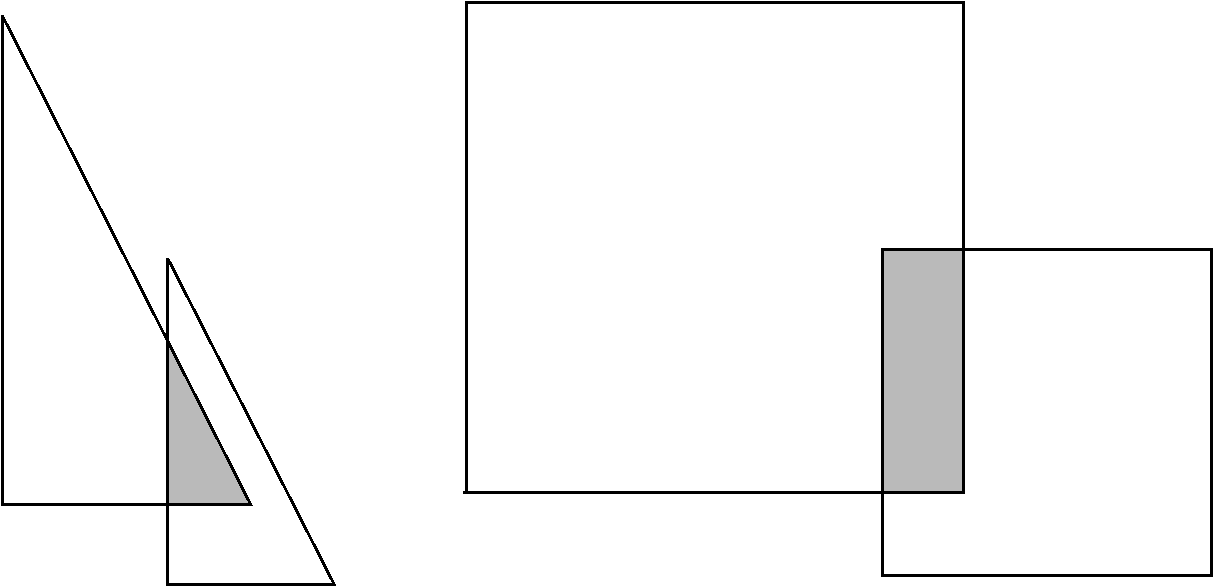
\includegraphics{Images/Img4.png}
    \caption{The intersection of $x+\CC$ and $y+\CC$ with a fixed hyperplane.}
    \label{fig:ch2_7.1}
\end{figure}

\section{Exercises and further results}\label{ch2_sec8}

\begin{exercise}\label{ex:ch2_1}
Show that a point is regular for the complement of a domain $D$ in the probabilistic sense if and only if it is regular for $D^c$ in the analytic sense.
\end{exercise}

\begin{exercise}\label{ex:ch2_2}
Give an example of a bounded domain $D$ and $f$ continuous on $\partial D$ such that the Dirichlet problem has no solution.
\end{exercise}

\begin{exercise}\label{ex:ch2_3}
Show that if $f$ is continuous, it is lower semicontinuous. Show that if $f_n$ are lower semicontinuous and $f_n \uparrow f$, then $f$ is lower semicontinuous. Show that if $f$ is lower semicontinuous, then $\liminf_{x\to y} f(x) \geq f(y)$.
\end{exercise}

\begin{exercise}\label{ex:ch2_4}
Prove Liouville's theorem\index{Liouville's theorem}: if $h$ is harmonic on $\R^d$, $d \geq 1$, and $h$ is bounded below, then $h$ is constant.
\end{exercise}

\begin{exercise}\label{ex:ch2_5}
Suppose $D$ is a bounded domain (not necessarily regular for the Dirichlet problem). If $f$ is continuous on $\partial D$, let
\begin{align*}
    H(f) &= \sup\{w : w~\text{is superharmonic on}~D, \\
    &\qquad\qquad\limsup_{x\to y} w(x) \leq f(y)~\text{for all}~y \in \partial D\}.
\end{align*}
The Dirichlet problem for $D$ with boundary values $f$ is resolutive\index{Resolutive} if $H(f) = -H(-f)$. Show that if the Dirichlet problem for $D$ with boundary values $f$ is resolutive, then $H(f)(x) = \E^x f(X_{T_D})$.
\end{exercise}

\begin{exercise}\label{ex:ch2_6}
Suppose $d = 2$, $D$ is a domain, and $y \in \partial D$. Show that if there exists a line segment contained in $D^c$ with one endpoint at $y$, then $y$ is regular for $D^c$.
\end{exercise}

\begin{exercise}\label{ex:ch2_7}
The generalized Laplacian\index{Generalized Laplacian} $\widetilde{\Delta}$ is defined by
\[
    \widetilde{\Delta}f(x) = \lim_{r\to 0} r^{-2} \int_{\partial B(0,r)}[f(x + y) - f(x)]\sigma_r(dy),
\]
provided the limit exists, where $\sigma_r$ is normalized surface measure on $\partial B(0,r)$. Show that if $f \in C^2$, then $\widetilde{\Delta}f(x) = \Delta f(x)$.
\end{exercise}

\begin{exercise}\label{ex:ch2_8}
Show that if $h$ is a Lipschitz function, then the partial derivatives of $h$ exist for a.e.\ point $x$.

\hint  Hold $x^1,\ldots,x^{i-1},x^i,\ldots,x^d$ fixed and use the one dimensional result.
\end{exercise}

\begin{exercise}\label{ex:ch2_9}
If $\mu$ is a finite measure on the boundary of a domain $D$, show there exist functions $f_n$ that are continuous on $\partial D$ such that $f_n(y)dy$ converges weakly to $\mu$.

\hint Cf.\ construction in Proposition \ref{prop:ch2_7.9}.
\end{exercise}

\begin{exercise}\label{ex:ch2_10}
If $(\P^x, X_t)$ is $d$-dimensional Brownian motion, $A$ is a Borel set, and $t > 0$, show there exists $B \in \FC_{t+}^{00}$ (defined in Sect.\ \chapref[I]{ch1_sec3}) such that the symmetric difference of $(T_A \leq t)$ and $B$ is $\R^x$-null for every $x$.

\hint Verify that it suffices to show that $(D_A \circ \theta_s \leq t)$ differs from a $\FC_{t+}^{00}$ set by a set that is $\P^x$-null for all $x$ (cf.\ the proof of Theorem \ref{thm:ch2_2.8}). Define
\[
    \P^\mu(\cdot) = \int \R^y(\cdot)(2\pi)^{-d/2}e^{-|y|^2/2}dy.
\]
Show that a consequence of Theorem \ref{thm:ch2_2.8} is that there exist $B_1$ and $B_2$ in $\FC_{t+}^{00}$ such that $B_1 \circ \theta_s \subseteq (D_A \circ \theta_s \leq t) \subseteq B_2 \circ \theta_s$ and $\P^\mu(B_2 - B_1) = 0$. Then
\begin{align*}
    \P^x(B_2 \circ \theta_s - B_1 \circ \theta_s) &= \E^x\P^{X_s}(B_2 - B_1) \\
    &= \int \P^y(B_2 - B_1)(2\pi s)^{-d/2}e^{-|y-x|^2/2s}dy.
\end{align*}
Now use the fact that $\int \P^y(\cdot)(2\pi s)^{-d/2}e^{-|y-x|^2/2s}dy$ is absolutely continuous with respect to $\P^\mu$.
\end{exercise}

\begin{exercise}\label{ex:ch2_11}
Show that if $B$ is a Borel set and $(\P^x, X_t)$ is $d$-dimensional Brownian motion, then $\P^x(T_B = t) = 0$ for each $x$ and each $t > 0$.
\end{exercise}

\begin{exercise}\label{ex:ch2_12}
Show that if $B$ is a Borel set, then $B^r$ is also a Borel set.
\end{exercise}

\begin{exercise}\label{ex:ch2_13}
Give examples of $\nu_1$ and $\nu_2$ such that (a) $\nu_1$ has density with respect to Lebesgue measure, but $U\nu_1(0) = \infty$, and (b) $U\nu_2$ is bounded but not continuous.
\end{exercise}

\mpagebreak

\begin{exercise}\label{ex:ch2_14}
Let $X_t$ be one-dimensional Brownian motion killed on exiting $D = (0,1)$. Let
\[
    g(x,y) = 2x(1-y) \wedge 2y(1-x).
\]
Show that if $f$ is bounded and measurable on $D$, then
\[
    \int_D f(y)g(x,y)dy = \E^x \int_0^{T_D} f(X_s)ds, \qquad x \in D.
\]
\end{exercise}

\begin{exercise}\label{ex:ch2_15}
Suppose $D$ is a domain and fix $x \in D$. Suppose $g(y)$ is $0$ if $y \in (B^c)^r$ and $g(y)$ is equal to $u(x,y)$ minus a positive harmonic function. Show $g$ must be equal to the Green function\index{Green function!One-dimensional Brownian motion} for $D$ with pole at $x$.
\end{exercise}

\begin{exercise}\label{ex:ch2_16}
Show that if $A \subseteq B$, then $g_A(x,y) \leq g_B(x,y)$ for all $x$ and $y$.
\end{exercise}

\begin{exercise}\label{ex:ch2_17}
Suppose $d \geq 2$ and $(\P^x, X_t)$ is $d$-dimensional Brownian motion. Show there exists a constant $c$ such that if $x \in B(0,r)$, then $\E^xT_{B(0,r)} \leq cr^2$. Show there exists $c$ such that if $x \in B(0,r/2)$, then $\E^xT_{B(0,r)} \geq cr^2$.
\end{exercise}

\begin{exercise}\label{ex:ch2_18}
Show that if $f$ is bounded with compact support, then $Uf$ is continuous.
\end{exercise}

\begin{exercise}\label{ex:ch2_19}
If $C$ is Newtonian capacity, show that $C(B) = 0$ implies $|B| = 0$. An event that occurs everywhere except for a set of capacity $0$ is said to occur quasi-everywhere\index{Quasi-everywhere}, written ``q.e.''
\end{exercise}

\begin{exercise}\label{ex:ch2_20}
A set $A$ is thin\index{Thin} at $x$ if $x \notin A^r$. A set $A$ is thin if it is thin at every point of $A$. A set $A$ is semipolar if it is the countable union of thin sets. Show semipolar sets are polar.
\end{exercise}

\begin{exercise}\label{ex:ch2_21}
Prove Proposition \ref{prop:ch2_5.11}.
\end{exercise}

\begin{exercise}\label{ex:ch2_22}
Show a set $B$ is polar if and only if there exists a measure $\mu$ such that $U\mu$ is infinite on $B$ but not identically infinite.
\end{exercise}

\begin{exercise}\label{ex:ch2_23}
Show that if $B$ is a bounded Borel set, $\nu$ is concentrated on $B$, and $U\nu \leq 1$ on $B^r$, then $C(B) \geq \nu(B)$.

\hint As in the proof of Proposition \ref{prop:ch2_5.10}, $U\nu \leq U\mu_B$ on $\R^d$, where $\mu_B$ is the equilibrium measure on $B$. As in the proof of Proposition \ref{prop:ch2_5.8},
\[
    \nu(\R^d) = \int U\gamma_r \,d\nu = \int U\nu \,d\gamma_r \leq \int U\mu_B \,d\gamma_r = C(B).
\]
\end{exercise}

\begin{exercise}\label{ex:ch2_24}
Show that if $\nu$ gives positive mass to a polar set $B$, then $U\nu(x)$ must be infinite for at least one $x$.
\end{exercise}

\begin{exercise}\label{ex:ch2_25}
Prove the domination principle\index{Domination principle}: if $\mu$ is a measure concentrated on $B^r$ and $f$ is nonnegative, superharmonic, and $f \geq U\mu$ q.e.\ on $B$, then $f \geq U\mu$ for all $x \in \R^d$. (q.e.\ means except for a set of capacity $0$; see Exercise \ref{ex:ch2_19}.)
\end{exercise}

\begin{exercise}\label{ex:ch2_26}
If $f$ is nonnegative, $e^{-\alpha t}P_tf \leq f$ for all $t$, and $e^{-\alpha t}P_tf \to f$ pointwise as $t$ tends to $0$, $f$ is said to be $\alpha$-excessive\index{À1@$\alpha$-excessive}. Show $\alpha$-excessive functions are $\beta$-excessive if $\alpha < \beta$. Show that if $f$ is $\alpha$-excessive, there exist $g_m \geq 0$ such that $U^\alpha g_m \uparrow f$. Show $f(x) = \E^xe^{-\alpha T_B}$ is $\alpha$-excessive for every Borel set $B$.
\end{exercise}

\begin{exercise}\label{ex:ch2_27}
The fine topology\index{Fine topology} is the coarsest topology with respect to which all the $\alpha$-excessive functions are continuous. Show $G$ is open in the fine topology if and only if for all $x \in G$, $x$ is not regular for $G^c$. Give an example of a finely open set in $\R^d$, $d \geq 3$, that is not open.
\end{exercise}

\begin{exercise}\label{ex:ch2_28}
Suppose $f > 0$ is superharmonic on a domain $D$. Show that the greatest harmonic minorant of $f$ exists.
\end{exercise}

\begin{exercise}\label{ex:ch2_29}
Suppose $U\mu$ is finite for all $x$. Show there exists a continuous additive functional $A_t$ such that $\E^xA_\infty = U\mu(x)$ for all $x$.

\hint $U\mu(X_t)$ is a continuous supermartingale. Use the Doob-Meyer decomposition. (Some care is needed because here we have a family of probabilities $\{\P^x\}$, not just one probability.)
\end{exercise}

\begin{exercise}\label{ex:ch2_30}
Suppose $A_t$ is a continuous additive functional with $f(x) = \E^xA_\infty$ finite for all $x$. Show $f$ is excessive.
\end{exercise}

\begin{exercise}\label{ex:ch2_31}
Suppose $A_t$ and $B_t$ are two additive functionals with $\E^xA_\infty = \E^xB_\infty < \infty$ for all $x$. Show $A_t \equiv B_t$ for all $t$.

\hint Use the uniqueness part of the Doob-Meyer decomposition.
\end{exercise}

\begin{exercise}\label{ex:ch2_32}
Suppose $A_t$ and $B_t$ are two continuous additive functionals. Suppose $\int_0^\infty h(X_s)dA_s = 0$ whenever $h \geq 0$ and $\int_0^\infty h(X_s)dB_s = 0$. Show there exists $f \geq 0$ such that $B_t = \int_0^t f(X_s)dA_s$ for all $t$.

\hint Suppose first that $A_t \leq B_t$ and $B_t$ is strictly increasing. Let
\[
    Z_s = \liminf_{r\to 0} \frac{B_{s+r} - B_s}{A_{s+r} - A_s},
\]
and let $f(x) = \E^xZ_0$. In the general case, consider the densities of $A_t$ and $B_t$ with respect to $C_t = A_t + B_t + t$.
\end{exercise}

\begin{exercise}\label{ex:ch2_33}
In the notation of (6.4), show $P_Bf = \overline{R}_Bf$.
\end{exercise}

\begin{exercise}\label{ex:ch2_34}
Show that if $U\mu$ is harmonic on an open set $B$, then $\mu$ is supported on $B^c$.
\end{exercise}

\begin{exercise}\label{ex:ch2_35}
Let $A$ and $B$ be disjoint compact subsets of $\R^d$, $d \geq 3$. Solve the condenser problem\index{Condenser problem}: find a signed measure $\nu$ concentrated on $A\cup B$ such that $U\nu \geq 0$ on $\R^d$, $U\nu = 1$ on $B^r$ and $U\nu = 0$ on $A^r$.

\hint Imitate Proposition \ref{prop:ch2_5.8} to find $\nu$ such that
\[
    U\nu(x) = \P^x(T_B < T_A, T_{A\cup B} < \infty).
\]
\end{exercise}

\begin{exercise}\label{ex:ch2_36}
Show that the definition of the Martin boundary is independent of the choice of the approximating sequence $D_n$. Show that the Martin boundaries that arise from two different choices of $x_0$ are homeomorphic.
\end{exercise}

\begin{exercise}\label{ex:ch2_37}
Find a metric for the Martin compactification $D^*$.

\hint Let $x_n$ be a countable dense subset of $D$ and let
\[
    \rho(y,y') = \sum_n 2^{-n}[\big(M(x_n,y) - M(x_n,y')\big) \wedge 1].
\]
\end{exercise}

\begin{exercise}\label{ex:ch2_38}
Suppose $\CC$ is a cone and $f(ry) = rf(y)$ for all $r > 0$, $y \in \CC$. Show $f$ is convex if and only if $f(x + y) \leq f(x) + f(y)$ for all $x,y \in \CC$.
\end{exercise}

\begin{exercise}\label{ex:ch2_39}
Let $\CC$ be a vector lattice. Show $(a \wedge b) + c = (a + c) \wedge (b + c)$. Show that if $\SC$ is a subset of $\CC$ that is closed under addition and under the operation $\wedge$, then $\SC - \SC$ is closed under the operations $\wedge$ and $\vee$. ($\SC - \SC = \{a - b : a,b \in \SC\}$.)

\hint For the second assertion, show $\big((a - b) \wedge (c - d)\big) + (b + d) = (a + d) \wedge (c + b)$.
\end{exercise}

\begin{exercise}\label{ex:ch2_40}
Suppose $f$ is lower semicontinuous and bounded on a metric space $(S,\rho)$. Show there exist continuous functions $f_n$ such that $f_n \uparrow f$.

\hint Let $f_n(x) = \inf\{f(z) + n\rho(x,z) : z \in S\}$.
\end{exercise}

\begin{exercise}\label{ex:ch2_41}
Prove the uniqueness assertion of the Constantinescu-Cornea theorem.
\end{exercise}

\begin{exercise}\label{ex:ch2_42}
% Note: Initially this ex asked to prove (5.12).
Prove Theorem \ref{thm:ch2_5.15}.
\end{exercise}

\begin{exercise}\label{ex:ch2_43}
Show that if $H$ is the upper half-space in $\R^d$, $d \geq 1$, then the transition densities for Brownian motion killed on exiting $H$ is
\[
    p_H(t,x,y) = p(t,x,y) - p(t,\widetilde{x},y), \qquad x,y \in H,
\]
where $\widetilde{x} = (x^1,\ldots,x^{d-1},-x^d)$.

\hint By the independence of $X_t^d$ and $(X_t^1,\ldots,X_t^{d-1})$, it suffices to consider the case $d = 1$. If $X_t$ is one-dimensional Brownian motion, by translation invariance and symmetry,
\begin{align*}
    \P^x(X_t > y, \inf_{s\leq t} X_s > 0) &= \P^0(X_t < x - y, \sup_{s\leq t} X_s < x) \\
    &= \P^0(X_t < x - y) - \P^0(X_t < x - y, \sup_{s\leq t} X_s \geq x).
\end{align*}
By Theorem \chapref[I]{thm:ch1_3.8}, this is $\P^0(X_t < x-y)-\P^0(X_t > 2x-(x-y)) = \P^x(X_t > y) - \P^{-x}(X_t > y)$. Now differentiate with respect to $y$.
\end{exercise}

\index{Green function!Two-dimensional Brownian motion|(}

\begin{exercise}\label{ex:ch2_44}
Suppose $d = 2$, $X_t$ is two-dimensional Brownian motion, and $H$ is the upper half-plane. Let
\mpagebreak
\[
    g(x,y) = \frac{1}{\pi}\log(1/|x - y|) - \frac{1}{\pi}\log(1/|\widetilde{x} - y|), \qquad x,y \in H,
\]
where $\widetilde{x} = (x^1,-x^2)$ if $x = (x^1,x^2)$. Show that if $f$ is bounded and measurable on $H$, then
\[
    \int_H f(y)g(x,y)dy = \E^x\int_0^{T_H} f(X_s)ds, \qquad x \in H.
\]
This says that $g(x,y)$ can be considered the Green function for $H$.

\hint Integrate the conclusion of Exercise \ref{ex:ch2_43} over $t$ from $0$ to $\infty$, using the idea of \eqref{eq:ch2_3.23}.
\end{exercise}

\begin{exercise}\label{ex:ch2_45}
Suppose $d = 2$ and $X_t$ is two-dimensional Brownian motion. Let
\[
    g(x,y) = \begin{cases}
        -\frac{1}{\pi}\log|x - y| + \frac{1}{\pi}\log\Big|\frac{x}{|x|} - |x|y\Big|, & x \neq 0, \\
        -\frac{1}{\pi}\log|y|, & x = 0,
    \end{cases}
    \qquad x,y \in B(0,1).
\]
Show that if $f$ is bounded and measurable on $B(0,1)$, then
\[
    \int_{B(0,1)} f(y)g(x,y)dy = \E^x\int_0^{\tau_{B(0,1)}} f(X_s)ds, \qquad x \in B(0,1).
\]
This says that $g$ can be considered the Green function for $B(0,1)$. If $g(x,y)$ is defined by the same formula for $x,y \in B(0,1)^c$ and $f$ is bounded on $B(0,1)^c$, show that
\[
    \int_{B(0,1)^c} f(y)g(x,y)dy = \E^x\int_0^{T_{B(0,1)}} f(X_s)ds, \qquad x \in B(0,1)^c.
\]

\hint Use Exercise \ref{ex:ch2_44} and the Kelvin transform.
\end{exercise}

\index{Green function!Two-dimensional Brownian motion|)}

\begin{exercise}\label{ex:ch2_46}
Show that if $D$ is a bounded set and $P_t^D$ is defined by \eqref{eq:ch2_4.13}, then there exists $c$ independent of $t$ such that
\[
    \|P_t^D f\|_{L^2(D)} \leq c\|f\|_{L^2(D)}.
\]
\end{exercise}

\notessection
\addcontentsline{toc}{section}{Notes}

Much of Sect.\ \ref{ch2_sec1}, \ref{ch2_sec3}, \ref{ch2_sec4}, \ref{ch2_sec5}, and \ref{ch2_sec6} was adapted from \cite{PortStone1978}. See that reference for further information and for some of the history of these results. Another good reference for this material is the encyclopedic work of \cite{Doob1984}. \cite{Helms1969} is a reference to the analytic approach to potential theory, as is \cite{Werner1981}. The proof of the Choquet capacity theorem in Sect.\ \ref{ch2_sec2} was taken from \cite{DellacherieMeyer1975}, and the applications to hitting times from \cite{BlumenthalGetoor1968}. Our approach to the Feynman-Kac formula is that of \cite{Williams1979}, while our proof of the smoothness of potentials is from \cite{GilbargTrudinger1983}. The proof of Theorem \ref{thm:ch2_3.16} is taken from \cite{BassKhoshnevisan1992}. \cite{Yosida1960} provided the basis for the proof of the Hilbert-Schmidt expansion theorem. Our construction of the Martin boundary follows the outline given in \cite{Brelot1969}. Our proof of the Choquet theorem (or Choquet-Meyer theorem) used \cite{DellacherieMeyer1983}; the older book by \cite{Meyer1966} was also very useful. The idea of Fig.\ \ref{fig:ch2_7.1} came from \cite{Phelps1966}. Many of the exercises in Sect.\ \ref{ch2_sec8} originate from material in \cite{PortStone1978}. Exercises \ref{ex:ch2_27}, \ref{ex:ch2_29}, \ref{ex:ch2_30}, \ref{ex:ch2_31}, and \ref{ex:ch2_32} are based on results from \cite{BlumenthalGetoor1968}; see \cite{BenvenisteJacod1973} for a solution to Exercise \ref{ex:ch2_32}.